\documentclass[11pt]{article}
\usepackage[margin=1in]{geometry}
\usepackage{amsmath,amssymb,amsthm,mathtools}
\usepackage{microtype}
\usepackage{booktabs}
\usepackage{array}
\usepackage{float}
\usepackage{tikz}
\usepackage[hidelinks]{hyperref}

\hypersetup{
  pdftitle={The sharp exponential rate of singularity for symmetric Bernoulli matrices},
  pdfauthor={OpenAI},
  pdfsubject={Singularity probability of symmetric Bernoulli matrices},
  bookmarksdepth=2
}
\numberwithin{equation}{section}
\allowdisplaybreaks[2]
\setlength{\emergencystretch}{2em}
\setcounter{tocdepth}{1}

\newtheorem{theorem}{Theorem}[section]
\newtheorem{proposition}[theorem]{Proposition}
\newtheorem{lemma}[theorem]{Lemma}
\newtheorem{corollary}[theorem]{Corollary}
\theoremstyle{definition}
\newtheorem{definition}[theorem]{Definition}
\theoremstyle{remark}
\newtheorem{remark}[theorem]{Remark}

\newcommand{\R}{\mathbb R}
\newcommand{\Z}{\mathbb Z}
\newcommand{\F}{\mathbb F}
\newcommand{\E}{\mathbb E}
\newcommand{\ind}{\mathbf 1}
\newcommand{\bits}{\{0,1\}}
\DeclareMathOperator{\rank}{rank}
\DeclareMathOperator{\corank}{corank}
\DeclareMathOperator{\Span}{span}
\DeclareMathOperator{\aff}{aff}
\DeclareMathOperator{\Hom}{Hom}
\DeclareMathOperator{\im}{im}
\DeclareMathOperator{\coker}{coker}
\DeclareMathOperator{\Tr}{Tr}
\DeclareMathOperator{\diag}{diag}
\DeclareMathOperator{\dist}{dist}
\DeclareMathOperator{\supp}{supp}

\title{The sharp exponential rate of singularity\\
for symmetric Bernoulli matrices}
\author{OpenAI}
\date{October 3, 2026}

\begin{document}
\maketitle

\begin{abstract}
Let \(A_n\) be a symmetric \(n\times n\) matrix whose entries on and above
the diagonal are independent uniform signs. We prove
\[
 \Pr(\det A_n=0)=\left(\frac12+o(1)\right)^n.
\]
\end{abstract}

\tableofcontents
\clearpage

\section{Introduction}\label{sec:introduction}

Let \(A_n\) be a symmetric \(n\times n\) random matrix whose entries
on and above the diagonal are independent and uniform on \(\{-1,1\}\).
We study the probability that \(A_n\) is singular. A specified pair of
rows is equal with probability \(2^{-n}\): the \(n-2\) comparisons away
from the two diagonal positions and the two remaining diagonal
conditions are independent. Thus singularity already occurs at this
exponential scale.

\begin{theorem}\label{thm:main}
For the symmetric Bernoulli matrix \(A_n\),
\[
 \Pr(\det A_n=0)=\left(\frac12+o(1)\right)^n
                =2^{-n+o(n)}
 \qquad\text{as }n\to\infty.
\]
\end{theorem}

The corresponding problem for a matrix with all \(n^2\) entries
independent has a long history. Koml\'os proved that a matrix with
independent uniform \(0/1\) entries is nonsingular with probability
tending to one \cite{Komlos}. Tikhomirov proved the sharp rate
\((1/2+o(1))^n\) for independent uniform signs
\cite{Tikhomirov}. Symmetry changes the exposure of the matrix:
revealing a row also reveals entries in all later rows. Arguments
based on independent rows therefore need a different source of
anti-concentration.

Costello, Tao, and Vu proved that a random symmetric Bernoulli matrix
is nonsingular with probability tending to one, obtaining the bound
\(O(n^{-1/8+\delta})\) for every fixed \(\delta>0\)
\cite{CTV}. Their proof developed quadratic Littlewood--Offord
estimates to handle the dependence between a row and its matching
column. Nguyen improved the bound to \(O_C(n^{-C})\) for every fixed
\(C>0\) \cite{Nguyen}, and Vershynin obtained a bound of the form
\(\exp(-n^c)\) for the sign model, as a special case of his theorem
for a class of subgaussian ensembles \cite{Vershynin}. Further
quantitative advances for this model gave bounds
of the forms
\(\exp(-c n^{1/4}\sqrt{\log n})\) \cite{FerberJain},
\(\exp(-c\sqrt n)\) \cite{CamposMattosMorrisMorrison},
\(\exp(-c\sqrt n(\log n)^{1/4})\) \cite{JainSahSawhney}, and
\(\exp(-c\sqrt{n\log n})\) \cite{CJMSRevisited}.
Campos, Jenssen, Michelen, and Sahasrabudhe proved an exponential
bound \(\exp(-cn)\), using inverse Littlewood--Offord estimates for
conditioned random walks and the method of inversion of randomness
\cite{SymmetricExponential}. Related work gives
quantitative control of the least singular value
\cite{SymmetricLeastSingular} and of larger rank deficiencies
\cite{HanRank}. Theorem~\ref{thm:main} identifies the leading
exponential rate for the specified sign model.

Our proof begins with an exact reduction to symmetric matrices of
bits. A Schur complement converts the sign matrix in dimension \(n\)
to a binary matrix in dimension \(N=n-1\). A reduction to corank one
then turns singularity into a question about appending a new column to
a nonsingular matrix \(B\). The relevant bit columns \(z\) satisfy
both \(z^{\mathsf T}B^{-1}z\in\bits\) and
\(\|B^{-1}z\|_\infty\le1\). It suffices to prove that their expected
number is \(2^{o(N)}\).

For a typical matrix \(B\), the column count is controlled by an
arithmetic potential \(\Psi(B)\in[0,1]\), defined in
Section~\ref{sec:framework}. The discriminant group
\(G_B=\Z^m/B\Z^m\) carries the symmetric pairing
\[
 ([x],[y])\longmapsto x^{\mathsf T}B^{-1}y\pmod{\Z}.
\]
Admissible classes have zero self-pairing. We partition them so that
pairings within each part have controlled denominators, with the cost
expressed in terms of the invariant factors. A robust subset of a large
part yields a lattice of controlled covolume on the graph of \(B^{-1}\).
A cover for rational subspaces of controlled height makes rank estimates
simultaneous for the span selected from these columns. Comparing a lower
determinant bound from the pairing with an upper bound from typical rank
and spectral properties proves the column estimate. The reusable lattice
arguments control covolumes and count short vectors after removing a
determinant-minimizing sublattice; the Reverse Minkowski Theorem of Regev
and Stephens-Davidowitz~\cite{ReverseMinkowski} is applied to its
orthogonal quotient.

For a nonsingular extension of width one, the old and new discriminant
groups have a common quotient. A kernel count modulo prime powers uses
symmetry to restrict the possible layer changes, while retaining
prescribed layers forces the new column into an integer lattice. A
second application of the lattice tools bounds cube intersections
simultaneously for all such lattices; it compares the cost of specifying
bases of cube differences with the number of matrix entries they
constrain. Counting partial certificates of retained layers and
optimizing their size then pays for the increase of \(\Psi\) in a
conditional exponential moment. For extensions of width two, a gate
requires both new columns to be admissible, and the static column
estimate directly pays for the probability of this gate.

Finally, every nonsingular matrix admits a path of nonsingular principal
minors with steps of width one or two, with the width-two steps satisfying
the gate. A separate elementary estimate for retaining high layers,
together with a bound on coranks modulo all primes, uses a long initial
part of the path to make a large high-layer tail unlikely anywhere in
a short terminal window. Outside this exceptional event, if the potential
is small at a node in that
window, the local conditional estimate controls the terminal moment.
Otherwise a bounded auxiliary statistic decreases at every step except
those with substantial retention or an expensive width-two gate. Many
such steps are necessary, and their conditional probability bounds make
this alternative negligible. The long initial part controls the
high-layer tail, while the short window limits the accumulation of local
errors.

\section{The binary model and the proof framework}\label{sec:framework}

We first reduce the singularity probability to the expected size of a set
of possible new columns. We then introduce the potential that will control
this set and state the two estimates on which the rest of the proof rests.

\subsection{From signs to bits}

A \emph{binary matrix} of size \(m\) is a symmetric \(m\times m\) matrix
whose entries on and above the diagonal are independent and uniform on
\(\bits\). We write \(\mathbf B_m\) for a random binary matrix and use
ordinary letters for its realizations.

\begin{lemma}\label{lem:sign-bit}
For \(n\ge2\),
\[
 \Pr(\det A_n=0)=\Pr(\det\mathbf B_{n-1}=0).
\]
\end{lemma}

\begin{proof}
Put \(\epsilon=(A_n)_{11}\), multiply \(A_n\) by \(\epsilon\), and then
apply the diagonal congruence with diagonal
\[
 1,\ \epsilon(A_n)_{12},\ldots,\epsilon(A_n)_{1n}.
\]
The resulting first row and column consist of ones. Conditional on the
original first row, the lower principal block still has independent
uniform signs on and above its diagonal: every one of these signs has
only been multiplied by a sign determined by the first row. Its Schur
complement at the top left entry is therefore \(-2\mathbf B_{n-1}\).
The two operations and the Schur complement preserve singularity.
\end{proof}

For the remainder of the proof, \(N\) is a reference integer tending to
infinity and
\[
 \ell=\log\log N,\qquad
 \mathcal I_N=\{m\in\Z:N-N^{7/10}\le m\le N\}.
\]
The logarithm \(\log\) is natural, while \(\log_2\) and \(\log_N\) have
the indicated bases. Every constant exponent of \(\ell\) is fixed before
\(N\) tends to infinity. In particular,
\(\ell^D/\log N=o(\ell^{-A})\) for all fixed \(A,D>0\).
We write \([m]=\{1,\ldots,m\}\).

We say that a property of \(\mathbf B_m\) \emph{holds typically} if its
failure probability is at most \(2^{-Nf(N)}\), uniformly for
\(m\in\mathcal I_N\), for some \(f(N)\to\infty\). When the property is
stated only for nonsingular matrices, failure means nonsingularity
together with failure of the stated conclusion. The typical set may
depend on any fixed precision parameters in the statement. A finite
intersection of typical properties is again typical.

All unqualified ranks are over \(\R\). We will also use the following
fact over finite fields.

\begin{lemma}[Principal rank]\label{lem:principal-rank}
Let \(M\) be a symmetric matrix over a field, of rank \(r\). Then \(M\)
has a nonsingular principal submatrix of size \(r\).
\end{lemma}

\begin{proof}
Choose a matrix \(X\) whose \(r\) columns form a basis of the column
space of \(M\), and choose a left inverse \(T\) of \(X\). Since \(M\) is
symmetric, its row space is the row space of \(X^{\mathsf T}\). Thus
\[
 M=X S X^{\mathsf T},\qquad S=TMT^{\mathsf T}.
\]
The matrix \(S\) is symmetric and has rank \(r\). Choose \(r\) independent
rows of \(X\). On those indices the principal submatrix of \(M\) is a
product of three nonsingular \(r\times r\) matrices.
\end{proof}

\begin{lemma}[Corank tail]\label{lem:corank-tail}
Let \(\mathbb K\) be any field, and regard the bits of \(\mathbf B_m\)
as elements of \(\mathbb K\). For \(1\le k\le m\),
\[
 \Pr\bigl(\corank_{\mathbb K}\mathbf B_m\ge k\bigr)
 \le \sum_{j=k}^{m}\binom mj\,2^{-j(j+1)/2}.
\]
Consequently, uniformly for \(m\in\mathcal I_N\),
\[
 \Pr\bigl(\corank_{\mathbb K}\mathbf B_m>N^{3/5}\bigr)
 \le 2^{-\Omega(N^{6/5})}.
\]
The implicit constant in the last bound is independent of the field.
\end{lemma}

\begin{proof}
If the rank is \(m-j\), Lemma~\ref{lem:principal-rank} supplies a
nonsingular principal submatrix on some \(m-j\) indices. Reveal all
entries in the corresponding columns. The remaining symmetric
\(j\times j\) block is forced over \(\mathbb K\), since its Schur
complement must vanish. Each forced entry has at most one possible bit
value, so the conditional probability is at most \(2^{-j(j+1)/2}\).
Union over the choices of indices and over \(j\ge k\). For
\(j>N^{3/5}\), the factor \(2^{-j(j+1)/2}\) dominates the at most
\(2^m\) choices of indices and the \(m\) choices of \(j\).
\end{proof}

\begin{lemma}[Reduction to corank one]\label{lem:corank-reduction}
For the binary model in dimension \(N\),
\[
 \Pr(\det\mathbf B_N=0)
 \le 2^{o(N)}\Pr(\corank\mathbf B_N=1)
       +2^{-\Omega(N^{6/5})}.
\]
\end{lemma}

\begin{proof}
Let \(B\) have corank \(k\ge1\), and write \(K=\ker B\). Choose \(k-1\)
coordinates whose restrictions to \(K\) are independent linear
functionals. Flip the diagonal bit at each of those coordinates, and
write \(D\) for the diagonal matrix of the changes. Its selected
diagonal entries are all nonzero.

If \((B+D)v=0\), pairing this equation with every \(u\in K\) gives
\(u^{\mathsf T}Dv=0\). The chosen coordinate functionals on \(K\) are
independent, so the selected coordinates of \(v\) are zero. It follows
that \(Bv=0\). Conversely, every vector in \(K\) with these coordinates
zero lies in \(\ker(B+D)\). This subspace has dimension one. Hence
flipping \(k-1\) diagonal bits produces a matrix of corank one.

For every matrix with \(k\le N^{3/5}\), fix one such choice of
coordinates. Each resulting matrix has at most
\[
 \sum_{j\le \lceil N^{3/5}\rceil}\binom Nj
   =2^{O(N^{3/5}\log N)}=2^{o(N)}
\]
preimages, because a preimage is recovered by specifying the flipped
coordinates. All binary matrices are equally likely. The matrices of
larger corank have the probability bounded in
Lemma~\ref{lem:corank-tail}.
\end{proof}

\subsection{Admissible columns}

For a nonsingular binary matrix \(B\) of size \(m\), define
\begin{equation}\label{eq:admissible-set}
 \mathcal S(B)=
 \left\{z\in\bits^m:
 z^{\mathsf T}B^{-1}z\in\bits,\quad
 \|B^{-1}z\|_\infty\le1\right\}.
\end{equation}
Set \(\mathcal S(B)=\varnothing\) when \(B\) is singular. These are the
columns that can occur when a corank-one matrix is reduced by deleting
a largest coordinate of its kernel vector.

\begin{lemma}\label{lem:column-reduction}
One has
\[
 \Pr(\corank\mathbf B_N=1)
 \le N\,2^{-N}\,\E|\mathcal S(\mathbf B_{N-1})|.
\]
\end{lemma}

\begin{proof}
Suppose a symmetric matrix \(M\) of size \(N\) has corank one, and
choose \(0\ne v\in\ker M\). Delete an index \(i\) for which \(|v_i|\)
is largest. The resulting principal submatrix \(B\) is nonsingular.
Indeed, the adjugate of \(M\) is a nonzero scalar multiple of
\(vv^{\mathsf T}\), so its \(i\)-th diagonal entry is nonzero.

Write \(z\) for the column at \(i\) on the remaining indices and \(a\)
for its diagonal bit. The kernel equation and the Schur complement give
\[
 B^{-1}z=-v_{[N]\setminus\{i\}}/v_i,\qquad
 a=z^{\mathsf T}B^{-1}z.
\]
Thus \(z\in\mathcal S(B)\). For any fixed deleted index, conditional on
\(B\), the pair \((z,a)\) is uniform on \(\bits^{N-1}\times\bits\).
For each \(z\in\mathcal S(B)\), the displayed equality fixes \(a\).
The probability for that index is therefore
\(2^{-N}\E|\mathcal S(\mathbf B_{N-1})|\). Union over \(i\).
\end{proof}

It remains to prove
\begin{equation}\label{eq:column-target}
 \E|\mathcal S(\mathbf B_{N-1})|\le 2^{o(N)}.
\end{equation}
Indeed, Lemmas~\ref{lem:corank-reduction} and
\ref{lem:column-reduction} then give the upper bound \(2^{-N+o(N)}\)
for the binary singularity probability. A specified row of
\(\mathbf B_N\) is zero with probability \(2^{-N}\), which gives the
matching lower bound.

\subsection{A potential on the discriminant group}

For nonsingular \(B\), the finite abelian group
\[
 G_B=\Z^m/B\Z^m
\]
has order \(|\det B|\). It records the possible denominators of
\(B^{-1}z\) for integer \(z\). We now give a numerical measure of its
invariant factors.

For a finite abelian group \(G\), write its \(p\)-primary part as
\[
 G_p\cong\bigoplus_{i\ge1}\Z/p^{b_{p,i}}\Z,\qquad
 b_{p,1}\ge b_{p,2}\ge\cdots\ge0,
\]
where only finitely many exponents are positive. For \(e\ge1\), put
\[
 k_G(p,e)=\#\{i:b_{p,i}\ge e\},\qquad
 \nu_p=\frac{\log_N p}{N}.
\]
We call \((p,e)\) with \(k_G(p,e)>0\) a \emph{layer}, its integer
\(k_G(p,e)\) its \emph{height}, and \(\nu_p\) its \emph{weight}.
All sums over layers below are finite. The identity
\begin{equation}\label{eq:group-order}
 \sum_{p,e} k_G(p,e)\nu_p=\frac{\log|G|}{N\log N}
\end{equation}
follows from \(\sum_e k_G(p,e)=\sum_i b_{p,i}\).
Hadamard's inequality gives \(|\det B|\le N^{N/2}\) for a binary
matrix of size \(m\le N\). Hence the sum in
Equation~\eqref{eq:group-order} is at most \(1/2\) for \(G_B\) and
for every quotient of \(G_B\).

Write \(k_B(p,e)=k_{G_B}(p,e)\), set \(\beta=7/5\), and define
\begin{equation}\label{eq:potential}
 \Psi(B)=\sum_{p,e}\nu_p\,\phi(k_B(p,e)),\qquad
 \phi(0)=\phi(1)=0,\quad
 \phi(2)=\beta,\quad
 \phi(k)=2k\quad(k\ge3).
\end{equation}
In particular \(0\le\Psi(B)\le1\), since \(0\le\phi(k)\le2k\).
We set \(\Psi(B)=0\) for singular \(B\) when an expression also
contains a nonsingularity indicator.

For example, a \(p\)-primary part with positive cyclic exponents
\((5,3,1)\) has
\[
 (k_B(p,1),\ldots,k_B(p,5))=(3,2,2,1,1),
\]
so this primary part contributes \((6+2\beta)\nu_p\) to \(\Psi(B)\).
Figure~\ref{fig:layers} depicts these layers. The coefficient
\(\beta=7/5\) exceeds the coefficient \(5/4\) in the height-two term of
the color-cost bound in Section~\ref{sec:discriminant}, while satisfying
the scalar budget inequality in Section~\ref{sec:potential-step}.

The potential is chosen to support two estimates. The first relates
the number of admissible columns to the arithmetic structure of \(B\).

\begin{proposition}[Admissible-column estimate]\label{prop:admissible-potential}
For every fixed \(A>0\), typically for nonsingular binary matrices
\(B\) of size \(m\in\mathcal I_N\),
\[
 |\mathcal S(B)|\le 2^{N(\Psi(B)+\ell^{-A})}.
\]
\end{proposition}

The second estimate controls the potential in expectation.

\begin{proposition}[Potential moment]\label{prop:path-potential}
For a binary matrix of size \(N-1\),
\[
 \E\!\left[\ind_{\{\det\mathbf B_{N-1}\ne0\}}\,
            2^{N\Psi(\mathbf B_{N-1})}\right]\le 2^{o(N)}.
\]
\end{proposition}

These propositions imply Equation~\eqref{eq:column-target}. Indeed,
fix \(A>0\) in Proposition~\ref{prop:admissible-potential}. On its
typical set use that estimate, and on the exceptional set use
\(|\mathcal S(B)|\le2^N\). For a suitable \(f(N)\to\infty\),
\[
 \E|\mathcal S(\mathbf B_{N-1})|
 \le 2^{N\ell^{-A}}
     \E\!\left[\ind_{\{\det\mathbf B_{N-1}\ne0\}}\,
                2^{N\Psi(\mathbf B_{N-1})}\right]
       +2^{N-Nf(N)}
 =2^{o(N)}.
\]

Sections~\ref{sec:lattice-tools}--\ref{sec:discriminant} prove the static
estimate in Proposition~\ref{prop:admissible-potential} by combining the
discriminant pairing with lattice, rank, and spectral estimates.
Sections~\ref{sec:minor-moves}--\ref{sec:potential-step} prove a local
conditional estimate for extensions: certificate pricing handles width
one, while Proposition~\ref{prop:admissible-potential} directly pays for
the gate at width two. Section~\ref{sec:minor-paths} adds a separate
high-layer tail argument and combines these estimates along paths to
prove Proposition~\ref{prop:path-potential}.

\section{Lattice tools and robust subsets}\label{sec:lattice-tools}

The lattice estimates in this section serve two purposes. They count
short vectors after removing directions of small determinant, and they
show that a robust collection of cube points has a difference span of
small height. We first fix the determinant conventions needed for both
uses.

\subsection{Determinants, quotients, and rational height}

A lattice \(L\) is a discrete subgroup of a finite-dimensional
Euclidean space, considered inside its real span \(E=\Span L\).
Its rank is \(\dim E\). If \(b_1,\ldots,b_r\) is a basis of \(L\), its
\emph{determinant} is the Euclidean covolume
\[
 \det L=\det\bigl(\langle b_i,b_j\rangle_{i,j=1}^r\bigr)^{1/2}.
\]
We set \(\det\{0\}=1\). Sublattices may have smaller rank. The
saturation of a sublattice \(M\subset L\) is
\(\overline M=L\cap\Span M\); it is a lattice of the same rank, and
\[
 \det M=[\overline M:M]\det\overline M.
\]
We call \(M\) \emph{primitive}, or \emph{saturated}, when
\(M=\overline M\). A primitive sublattice has a basis that extends to
a basis of \(L\). The dual lattice is always taken in the span:
\[
 L^*=\{y\in E:\langle y,x\rangle\in\Z\text{ for all }x\in L\}.
\]
In particular, the dual of the rank-zero lattice is the rank-zero
lattice.

\begin{lemma}[Orthogonal lattice quotients]\label{lem:lattice-quotient}
Let \(L\) have rank \(r\) and span \(E\), and let \(K\subset L\) be a
primitive sublattice of rank \(k\), with \(F=\Span K\). Write
\(\pi_{F^\perp}\) for orthogonal projection from \(E\) onto
\(E\cap F^\perp\). The Euclidean realization
\[
 L/K:=\pi_{F^\perp}(L)
\]
is a lattice of rank \(r-k\), canonically isomorphic to the abstract
quotient, and
\[
 \det L=\det K\,\det(L/K),\qquad
 \det L^*=(\det L)^{-1}.
\]
The dual identities are
\[
 (L/K)^*=L^*\cap F^\perp,\qquad
 K^*=\pi_F(L^*),
\]
where \(\pi_F\) is orthogonal projection onto \(F\).
For any sublattice \(M\subset L/K\), its full preimage
\(\widetilde M=\{x\in L:\pi_{F^\perp}x\in M\}\) has rank
\(k+\rank M\) and satisfies
\[
 \det\widetilde M=\det K\,\det M.
\]
These assertions include \(k=0\), \(k=r\), and \(r=0\), with all
rank-zero determinants equal to one.
\end{lemma}

\begin{proof}
Extend a basis \(b_1,\ldots,b_k\) of \(K\) to a basis
\(b_1,\ldots,b_r\) of \(L\). The projected vectors
\(\pi_{F^\perp}b_{k+1},\ldots,\pi_{F^\perp}b_r\) form a basis of the
projected lattice. Splitting Euclidean volume into the factor in \(F\)
and the factor orthogonal to \(F\) gives the first determinant identity.
The Gram matrix of the dual basis is the inverse Gram matrix, giving
the identity for \(\det L^*\).

For \(y\in E\cap F^\perp\), the equality
\(\langle y,\pi_{F^\perp}x\rangle=\langle y,x\rangle\) gives
\((L/K)^*=L^*\cap F^\perp\). Projection of \(L^*\) to \(F\) is
contained in \(K^*\). Conversely, for \(w\in K^*\), prescribe on the
basis of \(L\) the integer values \(\langle w,b_i\rangle\) for
\(i\le k\) and zero for \(i>k\). The representing vector belongs to
\(L^*\), and its projection to \(F\) is \(w\). This proves the second
dual identity. Finally, lift a basis of \(M\) and adjoin the basis of
\(K\). The resulting basis of \(\widetilde M\) gives its rank and
determinant by the same volume factorization. Empty bases give all the
rank-zero cases.
\end{proof}

A subspace \(W\subset\R^m\) is \emph{rational} if it is spanned by
integer vectors. Its integer lattice \(\Lambda_W=W\cap\Z^m\) has
rank \(\dim W\), and its \emph{height} is
\[
 H(W)=\det\Lambda_W.
\]
Thus \(H(\{0\})=H(\R^m)=1\). We will also write
\(h(W)=\log_N H(W)\).

\begin{lemma}[Height submodularity]\label{lem:height-submodularity}
For rational subspaces \(U,V\subset\R^m\),
\[
 H(U+V)H(U\cap V)\le H(U)H(V).
\]
Consequently \(h(U+V)+h(U\cap V)\le h(U)+h(V)\).
Every rational subspace has height at least one, and, for fixed \(m\)
and \(C<\infty\), there are only finitely many rational subspaces
\(W\subset\R^m\) with \(H(W)\le C\). These statements include
rank-zero subspaces.
\end{lemma}

\begin{proof}
Put \(J=U\cap V\), and project orthogonally off \(J\).
The lattice \(\Lambda_J=\Lambda_U\cap\Lambda_V\) is primitive in
each of \(\Lambda_U,\Lambda_V,\Lambda_U+\Lambda_V\). For the last
assertion, if \(u+v\in J\) with \(u\in\Lambda_U\) and
\(v\in\Lambda_V\), then \(u,v\in J\).
The projected spans of \(U\) and \(V\) intersect trivially. If
\(\overline\Lambda_U,\overline\Lambda_V\) denote their projected
lattices, the union of bases of these lattices is therefore a basis
of their sum. Orthogonally projecting the second set of basis
vectors off the span of the first can only decrease its volume.
Hence
\[
 \det(\overline\Lambda_U+\overline\Lambda_V)
 \le \det\overline\Lambda_U\,\det\overline\Lambda_V.
\]
Lemma~\ref{lem:lattice-quotient} now gives
\[
 \det(\Lambda_U+\Lambda_V)\det\Lambda_J
 \le \det\Lambda_U\,\det\Lambda_V.
\]
The saturation of \(\Lambda_U+\Lambda_V\) is
\(\Lambda_{U+V}\), whose determinant is no larger. This proves the
height inequality, and taking \(\log_N\) proves its additive form.

For a rank-\(r\) rational subspace, wedge a basis of \(\Lambda_W\).
The resulting vector in \(\bigwedge^r\Z^m\) is determined up to sign,
has Euclidean norm \(H(W)\), and determines its supporting subspace
\(W\).
Its integer coordinates are not all zero, so its norm is at least
one. A bounded ball contains finitely many vectors of
\(\bigwedge^r\Z^m\), and there are only \(m+1\) possible ranks.
This proves the finiteness assertion. For \(r=0\), the exterior
vector is \(1\) and there is just the zero subspace.
\end{proof}

For a coordinate vector \(e_i\), both possible intersections
\(U\cap\Span(e_i)\) have height one.
Lemma~\ref{lem:height-submodularity} therefore also gives
\(H(U+\Span(e_i))\le H(U)\). The next identity expresses height
ratios as determinants of normal lattices; it will transfer height
minimization to bounds on all sublattices of a dual lattice.

\begin{lemma}[Normal lattices and height]\label{lem:normal-height}
Let \(V\subset U\subset\R^m\) be rational subspaces, and put
\(\Lambda=\Lambda_U^*\). The primitive normal lattice
\[
 \mathcal N_U(V)=\Lambda\cap V^\perp
\]
has rank \(\dim U-\dim V\), and
\[
 \pi_V(\Lambda)=\Lambda_V^*,\qquad
 \det\mathcal N_U(V)=\frac{H(V)}{H(U)}.
\]
More generally, for any sublattice \(M\subset\Lambda\), set
\(V_M=U\cap(\Span M)^\perp\). Then \(V_M\) is rational and
\[
 \det M=[\mathcal N_U(V_M):M]\frac{H(V_M)}{H(U)}
 \ge \frac1{H(U)}.
\]
For \(V=U\) the normal lattice has rank zero and determinant one;
for \(V=\{0\}\) it is \(\Lambda_U^*\). If \(M=\{0\}\), the displayed
index is one and the determinant formula gives one.
\end{lemma}

\begin{proof}
The lattice \(\Lambda_V\) is primitive in \(\Lambda_U\), so the
second dual identity in Lemma~\ref{lem:lattice-quotient} gives
\(\pi_V(\Lambda_U^*)=\Lambda_V^*\). Its kernel is
\(\mathcal N_U(V)\), a primitive sublattice of the asserted rank.
Factoring the determinant of \(\Lambda_U^*\) along this kernel gives
\[
 \frac1{H(U)}
 =\det\mathcal N_U(V)\,\det\Lambda_V^*
 =\frac{\det\mathcal N_U(V)}{H(V)}.
\]

An integer basis matrix for \(\Lambda_U\) gives a rational basis for
its dual by inverting its Gram matrix. Thus \(\Span M\), and hence
\(V_M\), is rational. The saturation of \(M\) in \(\Lambda\) is
exactly \(\mathcal N_U(V_M)\). The index formula for determinants
and the first part of the lemma give the final identity; the
inequality follows from \(H(V_M)\ge1\).
\end{proof}

\subsection{Gaussian counts and determinant minimization}

For a lattice \(L\) and \(s>0\), define its Gaussian mass by
\[
 \rho_s(L)=\sum_{x\in L}\exp\!\left(-\frac{\pi\|x\|^2}{s^2}\right).
\]
In rank zero this mass equals one. The following is the scaled form
of the Reverse Minkowski Theorem of Regev and
Stephens-Davidowitz~\cite[Theorem~1.2]{ReverseMinkowski}.

\begin{theorem}[Reverse Minkowski Theorem]\label{thm:reverse-minkowski}
Let \(L\) be a lattice of rank \(j\ge1\), and let \(T>0\). Suppose
that
\[
 \det M\ge T^{\rank M}\qquad\text{for every sublattice }M\subset L.
\]
With \(\tau_j=10(\log j+2)\), one has
\[
 \rho_{T/\tau_j}(L)\le\frac32.
\]
For a rank-zero lattice the Gaussian mass is one at every scale, so
the corresponding assertion is immediate.
\end{theorem}

\begin{proof}
Apply the cited theorem to \(T^{-1}L\) in its Euclidean span.
Every rank-\(t\) sublattice of \(T^{-1}L\) has determinant at least
one, and \(\rho_{1/\tau_j}(T^{-1}L)=\rho_{T/\tau_j}(L)\).
\end{proof}

Here \(\tau_j\) is bounded above and below by absolute multiples of
\(\log(2j)\). We will use the theorem both at its stated scale and
at larger scales, through the following consequences of Poisson
summation.

\begin{lemma}[Gaussian point counts]\label{lem:gaussian-count}
Let \(L\) be a rank-\(j\) lattice. For \(R\ge0\) and \(s>0\),
\[
 \#\{x\in L:\|x\|\le R\}
 \le \exp(\pi R^2/s^2)\rho_s(L).
\]
For \(s'\ge s>0\),
\[
 \rho_{s'}(L)\le (s'/s)^j\rho_s(L).
\]
In particular, under the hypotheses of
Theorem~\ref{thm:reverse-minkowski}, if \(s_0=T/\tau_j\), then for
every \(u\ge s_0\),
\[
 \#\{x\in L:\|x\|\le R\}
 \le\frac32\left(\frac{u}{s_0}\right)^j
       \exp(\pi R^2/u^2).
\]
When \(j=0\), the point count and every Gaussian mass are one; the
first inequality is immediate and the second is equality.
\end{lemma}

\begin{proof}
Each point of norm at most \(R\) contributes at least
\(\exp(-\pi R^2/s^2)\) to \(\rho_s(L)\), proving the first bound.
The Gaussian Poisson formula in the span of \(L\) is
\[
 \rho_s(L)=\frac{s^j}{\det L}\rho_{1/s}(L^*).
\]
The Gaussian mass is nondecreasing in its scale. Applying this fact
to \(1/s'\le1/s\) in the formula proves the second bound. The last
bound follows by using the first bound at scale \(u\), then the
second bound and Theorem~\ref{thm:reverse-minkowski}. The same
Poisson identity reads \(1=1\) in rank zero.
\end{proof}

We obtain the hypotheses of the Reverse Minkowski Theorem by removing
a sublattice that minimizes a normalized determinant. The optional
rank bound below quantifies how many directions can be removed when
all original sublattices already have a weaker determinant bound.
Extremal sublattices and canonical filtrations also occur in the
reduction theory of Euclidean lattices; see
Grayson~\cite[Section~1]{Grayson}. We need only the elementary
minimization statement below.

\begin{lemma}[Determinant-minimizing sublattice]\label{lem:det-minimizer}
Let \(L\) be a lattice and let \(T>0\). The quantity
\[
 \frac{\det M}{T^{\rank M}},\qquad M\subset L\text{ a sublattice},
\]
has a minimum, attained by a primitive sublattice \(L_0\). It
satisfies
\[
 \det L_0\le T^{\rank L_0},\qquad
 \det M\ge T^{\rank M}\quad\text{for every sublattice }M\subset L/L_0.
\]
If in addition \(T_0>T\), \(\Delta\ge0\), and
\[
 \det M\ge e^{-\Delta}T_0^{\rank M}
       \quad\text{for every sublattice }M\subset L,
\]
then
\[
 \rank L_0\le\frac{\Delta}{\log(T_0/T)}.
\]
For \(L=\{0\}\) the unique choice is \(L_0=\{0\}\), and every
assertion holds with rank zero and determinant one.
\end{lemma}

\begin{proof}
The rank-zero lattice has normalized determinant one. For a fixed
positive rank \(t\), the determinant of a sublattice is the norm of
the wedge of one of its bases in the discrete lattice
\(\bigwedge^t L\). There are only finitely many such norms at most
\(T^t\). Thus among all normalized determinants no greater than
one there are only finitely many values, and the minimum is
attained. Saturating a minimizer can only decrease its determinant
while preserving its rank, so a primitive minimizer may be chosen.
Comparison with the rank-zero lattice gives
\(\det L_0\le T^{\rank L_0}\).

For a sublattice \(M\subset L/L_0\), lift it to \(\widetilde M\)
as in Lemma~\ref{lem:lattice-quotient}. Minimality gives
\[
 \frac{\det L_0}{T^{\rank L_0}}
 \le
 \frac{\det\widetilde M}{T^{\rank L_0+\rank M}}
 =
 \frac{\det L_0\,\det M}{T^{\rank L_0+\rank M}},
\]
which proves the quotient bound. Under the additional hypothesis,
writing \(k=\rank L_0\), the two bounds on \(\det L_0\) give
\(e^{-\Delta}T_0^k\le T^k\). Taking logarithms proves the rank
bound.
\end{proof}

\subsection{Robust subsets and small determinants}

Let \(\mathcal A\) be a nonempty finite set with affine span \(F\).
For \(\rho>0\), call \(\mathcal A\) \emph{\(\rho\)-robust} if every
affine subspace \(E\subset F\) of codimension \(t\) satisfies
\[
 |\mathcal A\cap E|\le 2^{-\rho t}|\mathcal A|.
\]
Robustness is preserved by injective affine maps, since their
restrictions to the affine span preserve codimension.

\begin{lemma}[Robust cube extraction]\label{lem:robust-extraction}
Let \(\varnothing\ne\mathcal A\subset\bits^m\), let \(\rho>0\),
and put \(d=\dim\aff\mathcal A\). There is an affine restriction
\(\mathcal A_0=\mathcal A\cap F\), with
\(F=\aff\mathcal A_0\) of dimension \(r\), such that
\(\mathcal A_0\) is \(\rho\)-robust and
\[
 \log_2|\mathcal A_0|
 \ge \log_2|\mathcal A|-\rho(d-r)
 \ge \log_2|\mathcal A|-\rho m,
 \qquad
 \log_2|\mathcal A_0|\le r.
\]
For any fixed \(a_0\in\mathcal A_0\), the number of ordered
\(r\)-tuples \((a_1,\ldots,a_r)\in\mathcal A_0^r\) for which
\(a_1-a_0,\ldots,a_r-a_0\) are independent is at least
\[
 |\mathcal A_0|^r\prod_{t=1}^r(1-2^{-\rho t})
 \ge \bigl((1-2^{-\rho})|\mathcal A_0|\bigr)^r.
\]
When \(r=0\), \(\mathcal A_0\) is a singleton and the number of
empty ordered tuples is one.
\end{lemma}

\begin{proof}
Among all nonempty affine restrictions \(\mathcal Q\) of
\(\mathcal A\), choose one maximizing
\[
 |\mathcal Q|\,2^{-\rho\dim\aff\mathcal Q}.
\]
There are finitely many distinct restrictions. Replacing the
restricting affine space by \(\aff\mathcal Q\) preserves the
restriction, so write the maximizer as
\(\mathcal A_0=\mathcal A\cap F\), \(F=\aff\mathcal A_0\).
Comparison with \(\mathcal A\) gives the lower bounds for its size.

Let \(E\subset F\) have codimension \(t\). If
\(\mathcal A_0\cap E\ne\varnothing\), its affine span has dimension
at most \(r-t\), and the intersection is itself an affine
restriction of \(\mathcal A\). Maximality therefore gives
\[
 |\mathcal A_0\cap E|\,2^{-\rho\dim\aff(\mathcal A_0\cap E)}
 \le |\mathcal A_0|\,2^{-\rho r},
\]
which is the required robustness bound. Empty intersections satisfy
the bound as well. Choose \(r\) coordinate functionals independent
on the direction space of \(F\). Projection to those coordinates is
injective on \(F\), and maps \(\mathcal A_0\) into \(\bits^r\).
Thus \(|\mathcal A_0|\le2^r\).

Finally, after \(i\) independent differences have been chosen, their
affine span with \(a_0\) has codimension \(r-i\) in \(F\).
Robustness leaves at least
\((1-2^{-\rho(r-i)})|\mathcal A_0|\) choices for the next point.
Multiplication for \(i=0,\ldots,r-1\) gives the claimed count. The
empty product proves the rank-zero assertion.
\end{proof}

The next lemma bounds the determinant of the entire difference
lattice. Its affine-image form will also apply to graph lattices:
the only metric input is a bound on image differences.

\begin{lemma}[Determinant of a robust image lattice]\label{lem:robust-height}
Fix \(D>0\) and \(C_0>0\). For all sufficiently large \(N\), put
\(\rho=\ell^{-D}\). Let \(m\le N\), let
\(\varnothing\ne\mathcal A\subset\bits^m\) be \(\rho\)-robust on
its affine span \(F\) of dimension \(r\), and let
\(\Phi:F\longrightarrow\R^d\) be an injective rational affine map,
meaning that it maps rational points of \(F\) to rational points of
\(\R^d\). Suppose that
\[
 \|\Phi(a)-\Phi(b)\|\le C_0\sqrt N
       \qquad(a,b\in\mathcal A).
\]
For any \(a_0\in\mathcal A\), the group
\[
 L_\Phi=\sum_{a\in\mathcal A}\Z\bigl(\Phi(a)-\Phi(a_0)\bigr)
\]
is a rank-\(r\) lattice, independent of the choice of \(a_0\), and
\[
 \det L_\Phi\le \exp\bigl(O_{D,C_0}(N\ell)\bigr).
\]
In particular, with \(W=\Span(\mathcal A-\mathcal A)\),
\[
 H(W)\le \exp\bigl(O_D(N\ell)\bigr).
\]
If \(r=0\), both lattices in question have rank zero and determinant
one.
\end{lemma}

\begin{proof}
The finitely many image differences are rational vectors, so they have
a common denominator. Their integer span is therefore contained in a
scaled copy of \(\Z^d\) and is discrete. The linear part of \(\Phi\) is
injective on the direction space of \(F\), so this lattice has rank
\(r\). Changing \(a_0\)
does not change the generated group. The assertions are immediate
if \(r=0\); suppose \(r\ge1\).

Set \(T=(\log N)^4\), and choose \(L_0\subset L_\Phi\) by
Lemma~\ref{lem:det-minimizer}. Write
\(\Gamma=L_\Phi/L_0\) for its orthogonal quotient and
\(j=\rank\Gamma\). The quotient has
\(\det M\ge T^{\rank M}\) for every sublattice \(M\subset\Gamma\),
while
\(\det L_0\le T^{r-j}\). Fix \(a_0\), and project the vectors
\(\Phi(a)-\Phi(a_0)\) into \(\Gamma\). They have norm at most
\(C_0\sqrt N\). If \(j\ge1\), Lemma~\ref{lem:gaussian-count} at
scale \(T/\tau_j\) bounds the number \(M\) of distinct projections by
\[
 M\le\frac32
     \exp\!\left(\frac{\pi C_0^2N\tau_j^2}{T^2}\right)
 \le 2^{O_{C_0}(N/(\log N)^6)}.
\]
Here \(j\le r\le N\), so \(\tau_j=O(\log N)\). The same final
bound holds for \(j=0\), when \(M=1\).

The preimage in \(F\) of any one projection fiber is an affine
subspace of codimension \(j\). A largest fiber contains at least
\(|\mathcal A|/M\) points, whereas robustness bounds its size by
\(2^{-\rho j}|\mathcal A|\). It follows that
\[
 j\le\frac{\log_2 M}{\rho}
   =O_{C_0}\!\left(\frac{N\ell^D}{(\log N)^6}\right).
\]
The projected differences generate \(\Gamma\). Choose \(j\) of
them that are independent. Their integer span is a full-rank
sublattice of \(\Gamma\), so the index formula and Hadamard's
inequality give
\[
 \det\Gamma\le (C_0\sqrt N)^j.
\]
For \(j=0\) this is the equality \(1=1\). Factoring the determinant
along \(L_0\) now yields
\[
 \det L_\Phi
 \le T^{r-j}(C_0\sqrt N)^j,
 \qquad
 \log\det L_\Phi
 \le 4N\ell+
     O_{C_0}\!\left(\frac{N\ell^D}{(\log N)^5}\right).
\]
For fixed \(D\), the error is \(o(N\ell)\), which proves the stated
determinant bound.

For the identity map the difference norms are at most
\(\sqrt m\le\sqrt N\), and \(L_\Phi\) is a full-rank sublattice
of \(W\cap\Z^m\). Saturating therefore decreases its determinant,
giving \(H(W)\le\det L_\Phi\) and the asserted height bound.
\end{proof}

\section{A finite cover for subspaces of controlled height}\label{sec:low-height}

Lemmas~\ref{lem:robust-extraction} and \ref{lem:robust-height} allow us
to pass from a large subset of \(\bits^m\) to a robust subset, with loss
at most \(\rho N\) in its base-two logarithmic size for
\(\rho=\ell^{-D_1}\) and fixed \(D_1>0\), whose difference span \(W\)
satisfies \(H(W)\le \exp(O(N\ell))\). This span may depend on the matrix
under study, so a rank estimate for one fixed space is insufficient.
Theorem~\ref{thm:low-height-cover} replaces all such spans by a small
fixed list while changing the relevant ranks only slightly.
Proposition~\ref{prop:typical-ranks} uses this cover to obtain simultaneous
rank estimates.

For rational subspaces \(U,V\subseteq\R^m\), define their \emph{rank
distance} by
\[
 d(U,V)=\dim U+\dim V-2\dim(U\cap V).
\]
Thus \(d(U,V)\) is the sum of the codimensions of \(U\cap V\) in \(U\)
and \(V\). Recall that \(H(U)=\det(U\cap\Z^m)\), with \(H(0)=1\).
One also has \(d(U^\perp,V^\perp)=d(U,V)\). Passing through the common
subspace \(U^\perp\cap V^\perp\) shows that the nullities of a fixed
symmetric bilinear form restricted to \(U^\perp\times U^\perp\) and
\(V^\perp\times V^\perp\) differ by \(O(d(U,V))\); the same holds for
the ranks of columns projected to these spaces. This is the relation
needed to transfer the fixed-space rank estimates.

\begin{theorem}[Low-height cover]\label{thm:low-height-cover}
Fix \(D,A>0\). For all sufficiently large \(N\), and every integer
\(0\le m\le N\), there is a list \(\mathcal C_{m,N}\) of rational subspaces of
\(\R^m\), depending also on \(D,A\), such that
\[
 |\mathcal C_{m,N}|\le 2^{N^2\ell^{-A}}.
\]
Every rational subspace \(W\subseteq\R^m\) satisfying
\(H(W)\le\exp(N\ell^D)\) has
\[
 \min_{U\in\mathcal C_{m,N}}d(U,W)\le N\ell^{-A}.
\]
\end{theorem}

\begin{proof}
Choose a fixed \(B_0>D+A+2\), and put
\[
 a=\ell^{-B_0},\qquad h(U)=\log_N H(U),\qquad
 \Delta=\frac{N\ell^D}{a\log N}.
\]
Throughout the proof \(N\) is sufficiently large in terms of these
fixed parameters. In particular \(a=o(1)\) and \(1/\log N=o(a)\).
We will encode a space within distance \(\Delta\) of each eligible
\(W\), at a cost \(o(N^2\ell^{-A})\) bits.
We follow the coordinate equations of \(W\) by a nested chain of
minimizing spaces. The height budget limits the total dimension lost in
drops larger than one. A flag in the normal lattice encodes each drop,
and the minimizing inequalities ensure that few flag positions have a
large encoding cost. We then sum these costs over the chain.

\medskip\noindent\textbf{The minimizing chain.}
Let \(r=\dim W\). Choose \(r\) pivot coordinates on which the coordinate
projection of \(W\) is an isomorphism, and write \(W\) as the graph of
rational linear functions on these coordinates. Order the nonpivot
coordinates, and impose their graph equations one at a time. This gives
rational spaces
\[
 \R^m=P_0\supset P_1\supset\cdots\supset P_{m-r}=W.
\]
At a step with coordinate vector \(e\), one has
\(P_{s-1}=P_s\oplus\R e\). Every coordinate vector whose equation has
not yet been imposed belongs to \(P_s\).

For each \(s\), minimize
\[
 F_s(U)=h(U)+a\,d(U,P_s)
\]
over rational subspaces \(U\), write the minimum as \(E_s\), and let
\(U_s\) be the greatest minimizer under inclusion. We justify these
choices. By Lemma~\ref{lem:height-submodularity}, \(h(U)\ge0\), and only
finitely many rational spaces satisfy \(H(U)\le N^{am}\). Testing
\(U=0\) shows that a minimizer can be sought among those spaces, so the
minimum exists.
Lemma~\ref{lem:height-submodularity} and the inequality
\[
 d(U+V,P)+d(U\cap V,P)\le d(U,P)+d(V,P)
\]
show that the sum and intersection of two minimizers for \(F_s\) are
again minimizers. The displayed inequality follows from the dimension
identity for \(U,V\) and the inclusion
\((U\cap P)+(V\cap P)\subseteq (U+V)\cap P\).
Since the set of minimizers is finite, their sum is the greatest one.
Also \(U_0=\R^m\) and \(E_0=0\).

The minimizers descend with the graph spaces. In fact, if \(P'\subseteq
P\), then
\[
 d(U+V,P)+d(U\cap V,P')\le d(U,P)+d(V,P').
\]
Here the required inequality between intersection dimensions follows
from
\((U\cap P)+(V\cap P')\subseteq (U+V)\cap P\), whose two summands
intersect in \(U\cap V\cap P'\). Combining this inequality with
Lemma~\ref{lem:height-submodularity}, for \(U=U_{s-1}\) and \(V=U_s\),
gives
\[
 F_{s-1}(U_{s-1}+U_s)+F_s(U_{s-1}\cap U_s)
 \le E_{s-1}+E_s.
\]
Minimality gives the reverse inequality. Hence \(U_{s-1}+U_s\) is an
old minimizer, and greatestness implies \(U_s\subseteq U_{s-1}\).

Every unprocessed coordinate vector \(e\in P_s\) belongs to \(U_s\).
Indeed, Lemma~\ref{lem:height-submodularity}, together with
\(H(\R e)=1\) and \(H(U\cap\R e)\ge1\), gives
\[
 H(U+\R e)\le H(U).
\]
If \(e\notin U\) but \(e\in P_s\), adjoining \(e\) decreases
\(d(U,P_s)\) by one, contradicting minimality. The energies are
nondecreasing as well. For a step \(P_{s-1}=P_s\oplus\R e\), one has
\[
 d(U+\R e,P_{s-1})\le d(U,P_s).
\]
This follows directly by comparing the intersections after adjoining
\(e\): the new intersection contains
\((U\cap P_s)\oplus\R e\), while the dimensions of \(U\) and \(P_s\)
each increase by at most one. The height inequality just proved,
applied to \(U=U_s\), yields
\(E_{s-1}\le E_s\).

Testing the last objective at \(W\) gives \(E_{m-r}\le h(W)\). Therefore
\[
 d(U_{m-r},W)\le \frac{h(W)}a\le\Delta.
\]
Write \(c_s=\dim U_{s-1}-\dim U_s\) for the dimension drop at step \(s\),
and let \(z\) count the steps with \(c_s=0\). At such a step the old and
new minimizers coincide and contain the coordinate vector \(e\) being
processed. Their intersection with \(P_s\) has dimension one less than
their intersection with \(P_{s-1}\), so \(E_s-E_{s-1}=a\).
Consequently \(z\le h(W)/a\). Write
\(\dim U_{m-r}=r+\theta\). The distance bound gives
\(|\theta|\le h(W)/a\), while summing the drops gives
\(\sum_s c_s=m-r-\theta\). Since there are \(m-r\) steps,
\[
 \sum_{s:c_s\ge2}(c_s-1)=z-\theta\le \frac{2h(W)}a.
\]
It follows that
\begin{equation}\label{eq:multi-drop-budget}
 \sum_{s:c_s\ge2}c_s\le \frac{4h(W)}a\le4\Delta.
\end{equation}

\medskip\noindent\textbf{Normal flags for a transition.}
We next count the choices for a transition \(U_{\rm old}\supseteq
U_{\rm new}\) of drop \(c\ge1\), assuming \(U_{\rm old}\) is known.
Let \(P_{\rm old}\supset P_{\rm new}\) be the corresponding graph
spaces, and set
\[
 \Lambda=(U_{\rm old}\cap\Z^m)^*
\]
in the Euclidean span \(U_{\rm old}\), and let
\(K=\Lambda\cap U_{\rm new}^{\perp}\). This is a primitive rank \(c\)
sublattice of \(\Lambda\), and it determines \(U_{\rm new}\).
For a rational \(V\subseteq U_{\rm old}\), Lemma~\ref{lem:normal-height}
identifies the determinant of its primitive normal lattice as
\[
 \det(\Lambda\cap V^\perp)=\frac{H(V)}{H(U_{\rm old})}.
\]
If \(V\) has codimension \(t\) in \(U_{\rm old}\), the two rank
distances from \(V\) and \(U_{\rm old}\) to any fixed space differ by at
most \(t\). Comparing \(V\) with the old minimizer, and saturating any
sublattice of \(\Lambda\), therefore gives
\[
 h(V)-h(U_{\rm old})
 \ge a\bigl(d(U_{\rm old},P_{\rm old})-d(V,P_{\rm old})\bigr)
 \ge-at
\]
and hence
\[
 \det L\ge N^{-a\rank L}\qquad(L\subseteq\Lambda).
\]
If \(K'\subseteq K\) is primitive of rank \(t\), it is also primitive
in \(\Lambda\), and is the normal lattice of a rational space
\(V'\) with \(U_{\rm new}\subseteq V'\subseteq U_{\rm old}\).
The normal-height identity and comparison with the new minimizer give
\[
 h(U_{\rm new})-h(V')
 \le a\bigl(d(V',P_{\rm new})-d(U_{\rm new},P_{\rm new})\bigr)
 \le a(c-t).
\]
Thus
\begin{equation}\label{eq:cover-normal-balance}
 \frac{\det K}{\det K'}
 =\frac{H(U_{\rm new})}{H(V')}
 \le N^{a(c-t)}.
\end{equation}
These two bounds are the only restrictions on the transition used in
the count.

Choose a saturated flag
\[
 0=K_0\subset K_1\subset\cdots\subset K_c=K
\]
as follows. In the orthogonally projected quotient \(K/K_{i-1}\),
choose a shortest nonzero vector \(v_i\), put \(\mu_i=\|v_i\|\), and
let \(K_i/K_{i-1}\) be the lattice on its line. A shortest nonzero
vector is primitive, so \(K_i/K_{i-1}=\Z v_i\). Each \(K_i\) is
primitive in \(K\), hence also in \(\Lambda\). Put
\(y_i=\log_N\mu_i\). The determinant identity in
Lemma~\ref{lem:lattice-quotient} and Equation~\eqref{eq:cover-normal-balance}
give, for every suffix,
\begin{equation}\label{eq:cover-flag-suffix}
 \sum_{j=i}^c y_j\le a(c-i+1).
\end{equation}
The classical shortest-vector consequence of Minkowski's convex body
theorem in rank \(u\) is
\(\lambda_1(L)\le C\sqrt u\,(\det L)^{1/u}\), with an absolute \(C\).
Apply it to \(K_{i+u-1}/K_{i-1}\). The vector \(v_i\) is shortest even
in the larger lattice \(K/K_{i-1}\), and hence
\begin{equation}\label{eq:cover-flag-range}
 y_i\le \frac1u\sum_{j=i}^{i+u-1}y_j
       +\frac12\log_Nu+O(1/\log N)
 \qquad(1\le u\le c-i+1).
\end{equation}
Taking a full suffix in this inequality shows
\[
 y_i\le \frac12+a+O(1/\log N).
\]
In particular \(y_i\le1\) for large \(N\).

Call position \(i\) expensive if \(y_i>1/2-3a\). A flag of length
\(c\) has \(O(ac)\) expensive positions, and has none when \(c=1\).
For the latter assertion, Equation~\eqref{eq:cover-flag-suffix} gives
\(y_1\le a<1/2-3a\). For the general assertion, suppose an expensive
position exists, and partition the suffix from the first such position
into ranges, each starting at an expensive position and ending just
before the next one, or at the end. For a range of length \(u\),
Equation~\eqref{eq:cover-flag-range} gives
\[
 \sum_{\text{range}}(y_j-a)
 \ge u\left(\frac12-4a-\frac12\log_Nu-O(1/\log N)\right).
\]
For \(u\le N^{2/5}\), this is at least \(u/5\) for large \(N\).
For every \(u\le N\), it is at least \(-C_1au\), since
\(1/\log N=o(a)\). The total over the ranges is nonpositive by
Equation~\eqref{eq:cover-flag-suffix}. The total length of the short
ranges is thus \(O(ac)\). There are at most \(c/N^{2/5}=o(ac)\) long
ranges, and at most the total short length short ranges. This proves
the asserted count.

\medskip\noindent\textbf{Counting flag vectors.}
We count the vector at each flag position in a quotient determined by
the preceding choices. Put
\[
 \Pi=\Lambda/K_{i-1},
\]
again using orthogonal projection. A rank \(t\) sublattice \(\bar L\)
of \(\Pi\) lifts, together with \(K_{i-1}\), to a rank \(t+i-1\)
sublattice of \(\Lambda\). By Lemma~\ref{lem:lattice-quotient}, the
first normal balance bound, and
\(\det K_{i-1}=\prod_{j<i}\mu_j\le N^c\), it follows that
\begin{equation}\label{eq:cover-projected-determinants}
 \det\bar L\ge
 \frac{N^{-a(t+i-1)}}{\det K_{i-1}}
 \ge N^{-at-2c}.
\end{equation}
Apply Lemma~\ref{lem:det-minimizer} to \(\Pi\) with \(T=N^{-2a}\).
Fix a deterministic choice of its minimizing primitive sublattice
\(L_0\), so that this choice requires no additional encoding once
\(\Pi\) is known. If \(j_0=\rank L_0\), the rank-zero competitor and
Equation~\eqref{eq:cover-projected-determinants} imply
\[
 N^{-aj_0-2c}\le\det L_0\le N^{-2aj_0},
 \qquad j_0\le \frac{2c}{a}.
\]
All sublattices of the quotient \(\Omega=\Pi/L_0\) have determinant
at least \(N^{-2a}\) to their rank.

First encode the image of \(v_i\) in \(\Omega\). If \(\Omega\) has
rank zero this image is unique. Otherwise, because its rank is at most
\(N\), Lemma~\ref{lem:gaussian-count} applies at the common smaller
scale
\[
 s_0=\frac{N^{-2a}}{C_2\log(2N)}
\]
for a suitable absolute \(C_2\). For an inexpensive position,
\(\mu_i\le N^{1/2-3a}\), and orthogonal projection does not increase
norm. Lemma~\ref{lem:gaussian-count} therefore bounds the base-two
logarithm of the number of images by
\begin{equation}\label{eq:cover-inexpensive-cost}
 O\bigl(1+N^{1-2a}\log^2N\bigr).
\end{equation}
For an expensive position the general bound on \(y_i\) permits a
common radius \(R=C_3N^{1/2+a}\), with an absolute \(C_3\). Use the
Gaussian comparison in Lemma~\ref{lem:gaussian-count} from \(s_0\)
to \(s_1=R/\sqrt N\). These satisfy \(s_1\ge s_0\) for large \(N\).
Writing \(k=\rank\Omega\le N\), the base-two logarithm of the count is
at most
\[
 O(1)+O(R^2/s_1^2)+k\log_2(s_1/s_0)
 \le O(N)+O\bigl(N(a\log N+\log\log N)\bigr)
 =O(aN\log N).
\]
The last equality uses \(a\log N\gg\log\log N\).

It remains to count the vectors above one fixed image in \(\Omega\).
Use the common radius \(R=C_3N^{1/2+a}\) for both kinds of position,
and let \(\mathcal V\) be the vectors \(v\in\Pi\) above that image with
\(\|v\|\le R\). If \(\mathcal V\) is nonempty, its differences lie in
\(L_0\). Let \(F\) be their real span, of dimension
\[
 j\le j_0\le 2c/a,\qquad j\le N.
\]
The intersection lattice \(L_F=\Pi\cap F\) has rank \(j\), and
Equation~\eqref{eq:cover-projected-determinants} gives
\(\det L_F\ge N^{-aj-2c}\). If \(j=0\), there is at most one vector.
Otherwise choose \(j\) independent differences in \(\mathcal V\),
each of norm at most \(2R\), and let \(L'\subseteq L_F\) be their
integer span. Fix \(v_0\in\mathcal V\). Within each coset of \(L'\)
in \(v_0+L_F\), the translates at the points of \(\mathcal V\) of a
half-open fundamental parallelepiped for these differences are disjoint
up to boundaries. They lie in the \(j\)-dimensional ball centered at
\(v_0\) of radius \(2(1+j)R\). Writing \(B_j(r)\) for the Euclidean
\(j\)-ball of radius \(r\), we may sum over the
\([L_F:L']=\det L'/\det L_F\) cosets to obtain
\[
 |\mathcal V|
 \le \frac{\operatorname{vol}_j B_j(2(1+j)R)}{\det L_F}.
\]
Since \(j\le N\) and \(R=O(N^{1/2+a})\), the logarithm of the
numerator is \(O(j\log N)\). The determinant bound consequently gives
\begin{equation}\label{eq:cover-fiber-cost}
 \log_2|\mathcal V|
 \le O((j+c)\log N)
 =O\left(\frac ca\log N\right).
\end{equation}
This bound is uniform over the fixed image and the preceding flag
choices.

The image and fiber choices specify \(v_i\in\Pi\). They also specify
\(K_i\): for any lift \(\widetilde v_i\in\Lambda\),
\[
 K_i=\Lambda\cap\Span(K_{i-1},\widetilde v_i).
\]
Thus the encoding reconstructs the next quotient and ultimately
\(K\), and hence \(U_{\rm new}\). The counts above can be applied
successively to the prefixes of all encodings of actual minimizing
chains; only such prefixes need satisfy the balance bounds.

\medskip\noindent\textbf{Total encoding cost.}
We finish by summing the costs. Specifying the pivot and coordinate
order, the drops, and the expensive positions costs \(O(N\log N)\)
bits. There are at most \(N\) flag positions altogether, because the
sum of all drops is at most \(m\). Put
\[
 S=\sum_{s:c_s\ge2}c_s\le4\Delta
\]
by Equation~\eqref{eq:multi-drop-budget}. The expensive-position
count gives at most \(O(aS)\) such positions over the whole chain;
there are none in drops of size one. For a drop \(c\), the \(c\)
fiber costs in Equation~\eqref{eq:cover-fiber-cost} total
\(O(c^2\log N/a)\). Using
\(\sum_{s:c_s\ge2}c_s^2\le S^2\), the full base-two logarithmic cost is
therefore bounded as follows. The four terms in the first bound account,
respectively, for the choices of pivots, order, drops, and positions;
for inexpensive images; for expensive images; and for fibers:
\[
 \begin{split}
 O(N\log N)
 &+O\bigl(N(1+N^{1-2a}\log^2N)\bigr)
   +O(a^2N\log N\,S)\\
 &+O\left(\frac{\log N}{a}(S^2+N)\right)\\
 &\le
 O\bigl(N^2N^{-2a}\log^2N\bigr)
 +O(aN^2\ell^D)
 +O\left(\frac{N^2\ell^{2D}}{a^3\log N}\right)
 +O\left(\frac{N\log N}{a}\right).
 \end{split}
\]
Each term is \(o(N^2\ell^{-A})\). For the first,
\(N^{-2a}\log^2N=\exp(-2\log N/\ell^{B_0}+2\ell)
=o(\ell^{-A})\). The second has factor
\(a\ell^D=\ell^{D-B_0}=o(\ell^{-A})\). For the third,
\(\ell^{2D}/(a^3\log N)=\ell^{2D+3B_0}/\log N=o(\ell^{-A})\);
the fourth follows from
\(\ell^{B_0}\log N/N=o(\ell^{-A})\). All exponents here are fixed
before \(N\) tends to infinity.

Collect the terminal spaces decoded by all these encodings, removing
duplicates. This is a list independent of \(W\), of size at most
\(2^{N^2\ell^{-A}}\) for sufficiently large \(N\). Every eligible
\(W\) contributes an encoding whose terminal space satisfies
\[
 d(U_{m-r},W)\le\Delta
 =\frac{N\ell^{D+B_0}}{\log N}
 =o(N\ell^{-A}).
\]
The required distance bound follows, uniformly for \(m\le N\).
\end{proof}

\section{Typical rank and spectral properties}\label{sec:typical}

We derive three properties of binary matrices that will be used below.
The rank properties hold simultaneously on all rational subspaces of
the prescribed height and for all choices of columns. Their uniformity
comes from Theorem~\ref{thm:low-height-cover}, together with a rank test
over \(\F_2\). The spectral property has the same exceptional-probability
scale, although its proof uses concentration rather than a union bound.

For a real symmetric matrix \(B\) and a subspace \(U\subseteq\R^m\),
write \(B|_U\) for the bilinear form
\((u,v)\mapsto u^{\mathsf T}Bv\) restricted to \(U\times U\).
Its nullity is \(\dim U-\rank(B|_U)\). We write \(\pi_U\) for
orthogonal projection onto \(U\), and put
\(E_X=\Span\{e_i:i\in X\}\) for \(X\subseteq[m]\).

\subsection{Uniform rank tests}

We first record the finite-field estimate behind both rank assertions.
Let \(\mathcal B\) be a uniform symmetric bilinear form on \(\F_2^m\),
including independent diagonal entries, and let \(S,T\) be fixed
subspaces of dimensions \(b,a\), respectively, where \(b\le a\).
For \(1\le t\le b\),
\begin{equation}\label{eq:typical-f2-rank}
 \Pr\bigl(\rank(\mathcal B|_{S\times T})\le b-t\bigr)
 \le C_0\,2^{-t(t+1)/2},
\end{equation}
with an absolute constant \(C_0\). Indeed, such a rank deficiency
provides a \(t\)-dimensional subspace \(K\subseteq S\) with
\(\mathcal B(K,T)=0\). The number of possible \(K\) is
\[
 \binom bt_{\!2}
 =2^{t(b-t)}\prod_{i=0}^{t-1}
       \frac{1-2^{i-b}}{1-2^{i-t}}
 \le C_0\,2^{t(b-t)},
 \qquad
 C_0=\prod_{j=1}^{\infty}(1-2^{-j})^{-1}<\infty.
\]
For a fixed \(K\), set \(e=\dim(K\cap T)\). Choose a basis of the
intersection, extend it separately to bases of \(K\) and \(T\), and
then extend their union to a basis of \(\F_2^m\). A change of basis
preserves the uniform distribution on symmetric forms. In this basis,
the equations \(\mathcal B(K,T)=0\) specify
\[
 ta-\binom e2
\]
independent entries of the symmetric form. In fact there are \(ta\)
entries before using symmetry, and the only repetitions are the two
orders of each off-diagonal pair inside \(K\cap T\). Diagonal entries
in that intersection remain independent conditions, also in
characteristic two. Since \(e\le t\) and \(a\ge b\), the number of
conditions is at least \(tb-\binom t2\). A union bound over \(K\)
gives Equation~\eqref{eq:typical-f2-rank}. The event is empty if
\(t>b\).

\begin{proposition}[Uniform low-height rank tests]\label{prop:typical-ranks}
For every pair of fixed constants \(D,A>0\), there is a function
\(f_{D,A}(N)\to\infty\) such that the following holds for every
\(m\in\mathcal I_N\) and all sufficiently large \(N\), with probability
at least \(1-2^{-Nf_{D,A}(N)}\) for \(B=\mathbf B_m\).
Simultaneously for every rational subspace \(W\subseteq\R^m\) with
\(H(W)\le\exp(N\ell^D)\), one has
\begin{enumerate}
 \item
 \(\dim W^\perp-\rank(B|_{W^\perp})\le N\ell^{-A}\);
 \item for every coordinate set \(X\subseteq[m]\),
 \[
  \rank\bigl[\pi_{W^\perp}Be_i\bigr]_{i\in X}
  \ge \min\{|X|,m-\dim W\}-N\ell^{-A}.
 \]
\end{enumerate}
The ranks and the orthogonal projections in these conclusions are
over \(\R\); no nonsingularity assumption on \(B\) is needed.
\end{proposition}

\begin{proof}
For any rational subspace \(U\subseteq\R^m\), the lattice
\(U\cap\Z^m\) is primitive in \(\Z^m\). Consequently an integer
basis matrix \(C_U\) of this lattice has full column rank modulo two:
a basis of a primitive sublattice extends to a basis of \(\Z^m\).
If \(U,V\) are rational, the matrix of the tested form is the integer
matrix \(C_U^{\mathsf T}BC_V\). Its real rank is at least the rank of
its reduction modulo two, because a nonzero minor modulo two is an
odd, hence nonzero, integer minor. Moreover \(B\bmod 2\) is uniform
among symmetric matrices over \(\F_2\). Thus
Equation~\eqref{eq:typical-f2-rank} applies to the reductions of the
column spaces of \(C_U,C_V\), which have the same respective
dimensions as \(U,V\). Their intersection after reduction can be
larger than the reduction of \(U\cap V\); the intersection correction
in the preceding count accommodates this without any further
assumption.

The tests we need are \(U=V\), and \(V=E_X\). In the second case,
\[
 \rank\bigl[\pi_UBe_i\bigr]_{i\in X}
   =\rank(C_U^{\mathsf T}BC_{E_X}),
\]
where \(C_{E_X}\) consists of the coordinate vectors with indices in
\(X\). To see this equality, \(C_U^{\mathsf T}\) annihilates
\(U^\perp\) and is an isomorphism from \(U\) to \(\R^{\dim U}\).
It therefore detects exactly the rank after projection to \(U\).

We also need stability when the testing subspace changes. For fixed
\(B\) and \(X\), define
\[
 \delta_0(U)=\dim U-\rank(B|_U),\qquad
 \delta_X(U)=\min\{|X|,\dim U\}
      -\rank(C_U^{\mathsf T}BC_{E_X}),
\]
where the second rank can equivalently be defined by the bilinear
form on \(U\times E_X\), without choosing an integer basis. If
\(Z\subseteq U\), restricting a matrix to \(Z\times Z\) deletes
\(\dim U-\dim Z\) rows and the same number of columns. Its rank
decreases by an amount between zero and twice that number. Hence
\[
 |\delta_0(U)-\delta_0(Z)|\le\dim U-\dim Z.
\]
For the form on \(U\times E_X\), the rank and the quantity
\(\min\{|X|,\dim U\}\) each decrease by an amount between zero and
\(\dim U-\dim Z\). The same inequality follows for \(\delta_X\).
Taking \(Z=U\cap V\) in these two inequalities gives
\begin{equation}\label{eq:typical-rank-stability}
 |\delta_0(U)-\delta_0(V)|\le d(U,V),\qquad
 |\delta_X(U)-\delta_X(V)|\le d(U,V).
\end{equation}
Here \(d(U,V)=\dim U+\dim V-2\dim(U\cap V)\), and the dimension
formula also gives \(d(U^\perp,V^\perp)=d(U,V)\).

Fix \(D,A\), put \(s=N\ell^{-A}\), and apply
Theorem~\ref{thm:low-height-cover} with precision exponent
\(P=2A+4\). For each \(m\in\mathcal I_N\), it gives a list
\(\mathcal C_m\) of rational subspaces with
\[
 |\mathcal C_m|\le 2^{N^2\ell^{-P}},\qquad
 \min_{V\in\mathcal C_m}d(W,V)\le N\ell^{-P}
\]
for every \(W\) in the height range of the proposition. Set
\(t=\lceil s/2\rceil\). Apply Equation~\eqref{eq:typical-f2-rank}
to \(U=V^\perp\) for every \(V\in\mathcal C_m\), both to its
restricted form and to its form against every \(E_X\). The comparison
of real and mod-two ranks above shows that the probability that any
of these real deficiencies is at least \(t\) is at most
\[
 C_0(1+2^m)\,2^{N^2\ell^{-P}-t(t+1)/2}
 \le 2^{-\Omega(N^2\ell^{-2A})}.
\]
In the last inequality, \(N^2\ell^{-P}=o(N^2\ell^{-2A})\) and
\(m=o(N^2\ell^{-2A})\), uniformly in the stated range of \(m\).
Tests whose smaller dimension is less than \(t\) need not be included.

Outside this event, choose a covering \(V\) for a given \(W\).
Equation~\eqref{eq:typical-rank-stability}, applied to their
orthogonal complements, bounds each deficiency for \(W\) by
\[
 t-1+N\ell^{-P}<s
\]
for all sufficiently large \(N\). This holds simultaneously for
all such \(W\) and all \(X\). Finally,
\(N\ell^{-2A}\to\infty\), so the displayed exceptional probability
has the form required in the statement.
\end{proof}

\begin{corollary}[Inverse restriction rank]\label{cor:inverse-rank}
For every pair of fixed constants \(D,A>0\), typically for nonsingular
binary matrices \(B\) of size \(m\in\mathcal I_N\), simultaneously
for every rational \(W\subseteq\R^m\) with
\(H(W)\le\exp(N\ell^D)\),
\[
 \rank(B^{-1}|_W)\ge\dim W-N\ell^{-A}.
\]
Here \(B^{-1}|_W\) is the restriction of the bilinear form with matrix
\(B^{-1}\), rather than the restriction of its associated linear map.
The exceptional probability is uniform in \(m\), as in
Proposition~\ref{prop:typical-ranks}.
\end{corollary}

\begin{proof}
The two radicals are
\[
 \operatorname{rad}(B|_{W^\perp})
   =W^\perp\cap B^{-1}W,
 \qquad
 \operatorname{rad}(B^{-1}|_W)
   =W\cap B(W^\perp).
\]
Since \(B\) is nonsingular, multiplication by \(B\) is an
isomorphism from the first space onto the second, with inverse
multiplication by \(B^{-1}\). Their dimensions are equal. The first
assertion of Proposition~\ref{prop:typical-ranks} therefore gives the
claimed rank for the inverse form, on the same typical set.
\end{proof}

\subsection{Corank modulo all primes}

For nonsingular \(B\) and every prime \(p\), the presentation of \(G_B\) gives
\[
 k_B(p,1)=\dim_{\F_p}(G_B/pG_B)
          =\corank_{\F_p}(B\bmod p).
\]
This dimension is the minimum number of generators of the \(p\)-primary
part, and \(k_B(p,e)\le k_B(p,1)\) for every \(e\). A uniform bound on
these coranks will therefore control the generators needed for quotients
of \(G_B\) and cap its layer heights.

\begin{proposition}[Uniform prime corank]\label{prop:prime-corank}
Typically for nonsingular binary matrices \(B\) of size
\(m\in\mathcal I_N\), one has, simultaneously for every prime \(p\),
\[
 \corank_{\F_p}(B\bmod p)\le N^{3/5}.
\]
More precisely, uniformly for \(m\in\mathcal I_N\), the probability
of nonsingularity together with failure of this assertion is at most
\(2^{-\Omega(N^{6/5})}\).
\end{proposition}

\begin{proof}
If \(B\) is nonsingular over \(\R\), its determinant is a nonzero
integer. Every prime at which its reduction has positive corank
divides that determinant. Hadamard's inequality gives
\[
 1\le |\det B|\le m^{m/2}\le N^{N/2},
\]
so it suffices to consider primes \(p\le N^{N/2}\). For each such
prime, Lemma~\ref{lem:corank-tail}, with field \(\F_p\), bounds the
probability of corank greater than \(N^{3/5}\) by
\(2^{-cN^{6/5}}\) for an absolute \(c>0\), uniformly in \(p\) and
\(m\). Even bounding the number of these primes by \(N^{N/2}\),
the union bound is
\[
 2^{(N/2)\log_2N-cN^{6/5}}
   \le 2^{-cN^{6/5}/2}
\]
for all sufficiently large \(N\). This also proves the asserted
uniformity.
\end{proof}

\subsection{Few eigenvalues near zero}

\begin{proposition}[Typical small-spectrum bound]\label{prop:typical-spectrum}
For every fixed \(A>0\), there is a fixed \(C_A>0\) and a function
\(f_A(N)\to\infty\) such that, for every \(m\in\mathcal I_N\) and
all sufficiently large \(N\), with probability at least
\(1-2^{-Nf_A(N)}\), the number of eigenvalues of \(B=\mathbf B_m\)
in
\[
 [-\sqrt N\,\ell^{-C_A},\ \sqrt N\,\ell^{-C_A}]
\]
is at most \(N\ell^{-A}\). Eigenvalues are counted with multiplicity.
One may take \(C_A=A+6\). This assertion does not require \(B\) to
be nonsingular.
\end{proposition}

\begin{proof}
\textbf{Mean bound.}
Let \(J_m\) be the all-ones matrix and write
\[
 2B=J_m+S,\qquad X=S/\sqrt m.
\]
The entries of \(S\) on and above the diagonal are independent uniform
signs. We first bound the number of eigenvalues of \(X\) in a short
interval about zero.

The limiting moments in the following calculation are those of
Wigner's semicircle law~\cite{Wigner}. We include the closed-walk
enumeration to obtain the quantitative error bound needed here. Let
\[
 d\mu_{\mathrm{sc}}(x)=\frac{1}{2\pi}\sqrt{4-x^2}\,
             \ind_{[-2,2]}(x)\,dx.
\]
For \(i\ge1\) with \(i+1\le m\),
\begin{equation}\label{eq:typical-walk-moments}
 \left|\frac1m\E\Tr X^{2i}
       -\int x^{2i}\,d\mu_{\mathrm{sc}}(x)\right|
 \le \frac{(2i+1)^{2i+2}}{m},
 \qquad
 \E\Tr X^{2i-1}=0.
\end{equation}
To prove it, expand the normalized trace as
\[
 \frac1m\E\Tr X^k
 =m^{-1-k/2}\sum_{v_0,\ldots,v_{k-1}\in[m]}
       \E\prod_{r=0}^{k-1}S_{v_rv_{r+1}},
 \qquad v_k=v_0.
\]
Each summand is a closed walk, with edges regarded as unordered and
loops allowed. Its expectation is one if every distinct edge is used
an even number of times, and is zero otherwise. This proves the
odd-moment assertion. For \(k=2i\), a contributing walk has at most
\(i\) distinct edges. Its graph is connected, and hence has at most
\(i+1\) vertices. Equality forces exactly \(i\) nonloop edges,
each used twice, forming a tree. When vertices are named in order of
first appearance, these walks are in bijection with Dyck words of
length \(2i\): the first traversal of a tree edge raises the depth,
and its return traversal lowers it. Their number is the Catalan number
\(\mathrm{Cat}_i=(i+1)^{-1}\binom{2i}{i}\), and each has
\((m)_{i+1}=m(m-1)\cdots(m-i)\) injective labelings.

The contribution of these tree walks is therefore
\(\mathrm{Cat}_i(m)_{i+1}/m^{i+1}\). Its difference from
\(\mathrm{Cat}_i\) is at most
\(\mathrm{Cat}_i i(i+1)/(2m)\), using
\(1-\prod_{h=0}^i(1-h/m)\le\sum_{h=0}^i h/m\).
Every remaining contributing walk has at most \(i\) vertices.
There are at most \((2i+1)^{2i}\) canonical vertex sequences, a
crude bound obtained by allowing each position any of \(2i+1\)
names. Each such sequence has at most \(m^i\) labelings and so
contributes at most \(1/m\) after normalization. Finally, elementary
beta integration gives
\[
 \int x^{2i}\,d\mu_{\mathrm{sc}}(x)
  =\frac{(2i)!}{i!(i+1)!}=\mathrm{Cat}_i,
\]
and its odd moments vanish. Combining these estimates, and using
\(\mathrm{Cat}_i\le4^i\), gives
Equation~\eqref{eq:typical-walk-moments}.

Fix the exponent \(A\) in the proposition and put
\[
 w=\ell^{-A-5},\qquad j=\lceil\ell^{2A+4}\rceil,
 \qquad f(x)=(1-|x|/w)_+,
 \qquad p_j(x)=2(1-x^2/16)^{2j}.
\]
For all large \(N\), \(f(x)\le p_j(x)\) for every real \(x\).
Outside \([-w,w]\) this follows from nonnegativity of the even
power. Inside that interval, Bernoulli's inequality gives
\[
 p_j(x)\ge 2(1-w^2/16)^{2j}
       \ge 2(1-jw^2/8)\ge1\ge f(x),
\]
because \(jw^2=O(\ell^{-6})\). All moments in \(p_j\) have degree
at most \(4j\), and \(2j+1\le m\) uniformly in
\(m\in\mathcal I_N\) for large \(N\). Expanding this polynomial
and applying Equation~\eqref{eq:typical-walk-moments} term by term,
the sum of the absolute values of its coefficients is
\(2(17/16)^{2j}\). Consequently
\[
 \left|\frac1m\E\Tr p_j(X)
        -\int p_j\,d\mu_{\mathrm{sc}}\right|
 \le \frac{2(17/16)^{2j}(4j+1)^{4j+2}}{m}
 =m^{-1+o(1)}.
\]
This estimate verifies the required growing degrees: indeed
\[
 j\log(j+1)=O_A(\ell^{2A+4}\log\ell)=o(\log m)
\]
uniformly in the stated range. In particular the last error is
\(o(\ell^{-A})\). On the support of \(\mu_{\mathrm{sc}}\),
\((1-x^2/16)^{2j}\le\exp(-jx^2/8)\) and the density is at most
\(1/\pi\). Thus
\[
 \int p_j\,d\mu_{\mathrm{sc}}
 \le \frac2\pi\int_{\R}e^{-jx^2/8}\,dx
 =O(j^{-1/2})=O(\ell^{-A-2}).
\]
The pointwise majorization now proves
\begin{equation}\label{eq:typical-tent-mean}
 \E\Tr f(X)=o(m\ell^{-A}),
\end{equation}
again uniformly in \(m\).

\medskip\noindent\textbf{Concentration and translation to \(B\).}
We next obtain concentration strong enough for typicality. Pointwise,
\[
 f(x)=1-g_1(x)+g_2(x),\qquad
 g_1(x)=|x|/w,\qquad g_2(x)=(|x|/w-1)_+.
\]
Both \(g_1,g_2\) are convex and \(1/w\)-Lipschitz. Their traces are
convex functions of a real symmetric matrix. For completeness, if
\(M_+\) denotes its spectral positive part, then
\[
 \Tr M_+=\max_{0\preceq P\preceq I}\Tr(PM).
\]
The identities
\[
 \Tr g_1(M)=w^{-1}\bigl(\Tr M_++\Tr(-M)_+\bigr),\qquad
 \Tr g_2(M)=\Tr(M/w-I)_++\Tr(-M/w-I)_+
\]
express each trace as a sum of suprema of affine functions of \(M\),
which proves convexity.

Let \(y=(y_{ab})_{a\le b}\) be an arbitrary real vector of independent
upper-triangular coordinates, and form \(X(y)=S(y)/\sqrt m\) by
symmetric reflection. For real symmetric matrices, the
Hoffman--Wielandt inequality~\cite[Theorem~1 and Remark~2]{HoffmanWielandt}, with their
eigenvalues ordered, states that
\[
 \sum_{i=1}^m|\lambda_i(M)-\lambda_i(M')|^2
       \le\|M-M'\|_F^2.
\]
It follows by Cauchy--Schwarz that for \(a=1,2\),
\[
 |\Tr g_a(X(y))-\Tr g_a(X(z))|
 \le\frac{\sqrt m}{w}\|X(y)-X(z)\|_F
 \le\frac{\sqrt2}{w}\|y-z\|_2.
\]
The last inequality uses
\(\|X(y)-X(z)\|_F^2\le(2/m)\|y-z\|_2^2\).
Thus each trace is convex and \(L\)-Lipschitz as a function of the
independent coordinates, with \(L=\sqrt2/w\).

Talagrand's convex Lipschitz concentration theorem on the product
cube~\cite[Theorem~3]{Talagrand} implies that, for universal \(c,C>0\),
if \(F:\R^d\to\R\) is convex and globally \(L\)-Lipschitz for the
Euclidean norm, then its value at independent uniform signs satisfies
\[
 \Pr(|F-\E F|>u)\le C\exp(-cu^2/L^2)\qquad(u\ge0).
\]
The usual statement about a median implies this form: integrating
its tail bounds the difference between the median and the expectation
by \(O(L)\), which can be absorbed by adjusting \(c,C\).
Apply the theorem to the two traces. By
Equation~\eqref{eq:typical-tent-mean}, their difference
\(\Tr f(X)=m-\Tr g_1(X)+\Tr g_2(X)\) has expectation at most
\(m\ell^{-A}/8\) for large \(N\). If it exceeds
\(m\ell^{-A}/4\), at least one of the two convex traces deviates
from its expectation by more than \(m\ell^{-A}/16\). Therefore
\begin{equation}\label{eq:typical-tent-tail}
 \Pr\bigl(\Tr f(X)>m\ell^{-A}/4\bigr)
 \le 2C\exp\bigl(-c' m^2\ell^{-2A}w^2\bigr)
 \le 2^{-c_A N^2\ell^{-4A-10}}
\end{equation}
for some \(c',c_A>0\) and all sufficiently large \(N\), uniformly
in \(m\). Since \(N\ell^{-4A-10}\to\infty\), this is a
\(2^{-Nf_A(N)}\) exceptional probability with \(f_A(N)\to\infty\).

On the complementary event, \(f\ge1/2\) on \([-w/2,w/2]\) shows
that \(X\) has at most \(m\ell^{-A}/2\) eigenvalues in that
interval. Finally \(2B/\sqrt m=X+J_m/\sqrt m\) is a rank-one
perturbation of \(X\). Eigenvalue interlacing changes the cumulative
eigenvalue count at either endpoint of an interval by at most one,
so it can increase the count in any interval by at most two. Take
\(C_A=A+6\). Uniformly for \(m\in\mathcal I_N\),
\[
 2\sqrt{N/m}\,\ell^{-C_A}\le w/2
\]
for all sufficiently large \(N\). The eigenvalues of \(B\) in the
interval of the proposition therefore number at most
\[
 \frac12m\ell^{-A}+2\le N\ell^{-A}.
\]
Together with Equation~\eqref{eq:typical-tent-tail}, this proves the
proposition.
\end{proof}

\section{The discriminant pairing and admissible columns}\label{sec:discriminant}

We prove Proposition~\ref{prop:admissible-potential}. The arithmetic
part of the proof colors isotropic elements of the discriminant group
so that the pairing on differences within one color has controlled
image order. The geometric part converts this order bound into a
dimension bound for a robust subset of admissible columns.

\subsection{Orthogonal blocks and a coloring of isotropic elements}

For a nonsingular symmetric integer matrix \(B\), the formula
\[
 \lambda_B(\bar x,\bar y)=x^{\mathsf T}B^{-1}y\bmod\Z
 \qquad(\bar x,\bar y\in G_B)
\]
defines a symmetric pairing with values in \(\mathbb Q/\Z\).
Changing \(x\) or \(y\) by a vector in \(B\Z^m\) changes the displayed
value by an integer. Moreover, if \(\lambda_B(\bar x,\bar y)=0\) for
every \(y\in\Z^m\), then \(B^{-1}x\in\Z^m\), so \(\bar x=0\).
Thus the induced map from \(G_B\) to
\(\Hom(G_B,\mathbb Q/\Z)\) is an isomorphism. We call such a pairing
\emph{perfect}.

Distinct primary components are orthogonal: a pairing value between
an element of \(p\)-power order and one of \(q\)-power order is
annihilated by coprime powers when \(p\ne q\). The restriction to each
primary component is consequently perfect. An element is
\emph{isotropic} if its self-pairing is zero. If an element of \(G_B\)
is isotropic, then so is its projection to each primary component,
by the uniqueness of primary decomposition in \(\mathbb Q/\Z\).
In particular the class of every \(z\in\mathcal S(B)\) is isotropic.

Orthogonal decompositions of these pairings are standard in the theory
of finite linking forms; see Miranda~\cite[Section~1]{Miranda}.
We include the elementary splitting argument and the precise block
forms needed here.

\begin{lemma}[Orthogonal block decomposition]\label{lem:discriminant-blocks}
Let \(G\) be a finite abelian \(p\)-group with a perfect symmetric
pairing \(\lambda:G\times G\to\mathbb Q/\Z\). It is an orthogonal
direct sum of blocks of the following forms:
\begin{enumerate}
 \item a cyclic group of order \(p^j\) whose generator has
 self-pairing \(a/p^j\bmod\Z\), with \(p\nmid a\);
 \item when \(p=2\), a group \((\Z/2^j\Z)^2\) with pairing matrix
 \[
  2^{-j}\begin{pmatrix}2a&c\\c&2d\end{pmatrix}\bmod\Z,
  \qquad c\ \text{odd}.
 \]
\end{enumerate}
\end{lemma}

\begin{proof}
Let \(p^j\) be the exponent of a nonzero group still to be split.
If some element has self-pairing of order \(p^j\), it has order
\(p^j\) and its cyclic subgroup is a block of the first kind.
Otherwise choose an element \(x\) of order \(p^j\). Perfectness
implies that the character \(\lambda(x,\cdot)\) has order \(p^j\),
so there is an element \(y\) for which \(\lambda(x,y)\) has order
\(p^j\). Write the three pairing values on \(x,y\), with denominator
\(p^j\), using numerators \(a,c,d\), respectively. Then \(c\) is
a unit modulo \(p\), while \(a,d\) are divisible by \(p\).
For odd \(p\), the self-pairing numerator of \(x+y\) is
\(a+2c+d\), a unit, so again a block of the first kind is available.

For \(p=2\), the two diagonal numerators are even and the
off-diagonal numerator is odd. The resulting two by two numerator
matrix is invertible modulo \(2^j\). Pairing a relation between
\(x,y\) with \(x,y\) therefore shows that its two coefficients
vanish modulo \(2^j\). Thus they span \((\Z/2^j\Z)^2\), and the
restriction of the pairing to this subgroup is perfect, giving the
second kind of block.

It remains to justify splitting a block \(H\) off orthogonally.
Because the pairing on \(H\) is perfect, for any \(g\in G\) there
is a unique \(h\in H\) such that
\(\lambda(g,\cdot)|_H=\lambda(h,\cdot)|_H\). Hence
\(g-h\in H^\perp\). Also \(H\cap H^\perp=0\), so
\(G=H\oplus H^\perp\). The pairing on \(H^\perp\) is perfect,
since an element annihilating both summands annihilates \(G\).
Iteration proves the decomposition.
\end{proof}

The exponents of the cyclic factors in this decomposition are the
invariant exponents \(b_1\ge b_2\ge\cdots\) of \(G\). A block of the
second kind contributes two equal exponents.

\begin{lemma}[Primary coloring]\label{lem:primary-coloring}
In the setting of Lemma~\ref{lem:discriminant-blocks}, put \(h=b_3\),
with zero exponents appended as necessary. In an orthogonal block
decomposition, let \(U\) be the sum of the blocks of exponent
strictly greater than \(h\), and let \(T\) be the remaining sum.
There is a coloring of the isotropic elements of \(G\) with \(C_p\)
colors such that elements \(x,y\) of one color satisfy
\begin{equation}\label{eq:primary-color-pairing}
 p^h\lambda_U(x_U,y_U)=0\quad\text{in }\mathbb Q/\Z.
\end{equation}
Here \(x_U,y_U\) denote the projections to \(U\). The color counts
may be chosen to satisfy
\[
 C_p\le 1+8b_1,\qquad
 C_p\le 2^{b_2-b_3}\quad\text{if \(p\) is odd}.
\]
\end{lemma}

The cutoff at \(b_3\) leaves at most two cyclic factors above it.
Up to a lower-order error, the color count will be charged to height-two
layers, while layers of height at least three will control the order of
the pairing image on differences within one color.

\begin{proof}
The exponent of \(T\) divides \(p^h\). Isotropy and orthogonality
therefore imply
\begin{equation}\label{eq:top-self-denominator}
 p^h\lambda_U(x_U,x_U)=0
\end{equation}
for every element under consideration. There are at most two cyclic
factors in \(U\). A block of the second kind cannot be divided by
the cutoff at \(h\), since its two factors have equal exponent.
We can thus handle all possibilities explicitly. In the following,
\(v_p(0)=+\infty\); for a nonzero cyclic coordinate its valuation is
that of any representative not divisible by the full modulus.

If \(U=0\), use one color. If it has one factor, this is a cyclic
block of exponent \(j>h\), with coordinate \(x\) and a unit
self-pairing numerator. Equation~\eqref{eq:top-self-denominator}
forces
\[
 v_p(x)\ge \left\lceil\frac{j-h}{2}\right\rceil.
\]
Two such coordinates have mutual pairing annihilated by \(p^h\),
so again one color suffices.

Suppose next that \(U\) consists of two orthogonal cyclic blocks of
exponents \(j\ge i>h\), with respective unit self-pairing numerators
\(a_1,a_2\). For their coordinates \(x,y\), put
\[
 F=\max\{j-2v_p(x),\,i-2v_p(y)\}.
\]
Use one \emph{deep} color for \(F\le h\). Two deep elements have the
required mutual denominator term by term, since the sum of the two
valuations in either coordinate is at least its exponent minus \(h\).
If \(F>h\), the two entries in the maximum must equal \(F\).
Otherwise the term of largest denominator in the self-pairing
could not cancel, contrary to
Equation~\eqref{eq:top-self-denominator}. In particular \(F\le i\),
and \(F\) has the parity of both \(i\) and \(j\). Write
\[
 x=p^{(j-F)/2}X,\qquad y=p^{(i-F)/2}Y,
\]
where \(X,Y\) are units. With \(n=F-h>0\), the self-pairing
condition is
\[
 a_1X^2+a_2Y^2\equiv0\pmod{p^n}.
\]
The residues of \(X,Y\) modulo \(p^n\) are well defined: they are
determined modulo \(p^{(j+F)/2}\) and \(p^{(i+F)/2}\), respectively,
and both exponents are at least \(F\ge n\).
Color this element by \(F\) and
\(r=XY^{-1}\bmod p^n\). Its ratio satisfies
\(r^2\equiv-a_2a_1^{-1}\pmod{p^n}\). For two elements with the
same color, using primes for the coordinates of the second one,
\[
 a_1XX'+a_2YY'
 \equiv YY'(a_1r^2+a_2)\equiv0\pmod{p^n}.
\]
This is precisely Equation~\eqref{eq:primary-color-pairing}.

For completeness, a unit square has at most two square roots modulo
an odd prime power and at most four modulo a power of \(2\).
Indeed, for two unit roots \(r,s\), the modulus divides
\((r-s)(r+s)\). At an odd prime at most one factor is divisible by
\(p\), giving \(r\equiv s\) or \(r\equiv-s\pmod{p^n}\). At \(2\),
for odd \(r,s\), one of \(r-s,r+s\) has valuation exactly one and
the other is divisible by four, with the convention of infinite
valuation at zero. For \(n\ge2\) this gives
\(r\equiv s\) or \(r\equiv-s\pmod{2^{n-1}}\), allowing at most four
residues modulo \(2^n\); \(n=1\) is immediate.

There are at most \(\lceil(i-h)/2\rceil\) possible nondeep values of
\(F\). At odd \(p\), the count is thus at most
\(1+2\lceil(i-h)/2\rceil\). For \(i-h\ge2\) this is at most
\(2^{i-h}\). If \(i-h=1\) and a nondeep element exists, its value
is \(F=h+1\). The parity just established shows that in a deep
element the two exponent-minus-twice-valuation quantities are at
most \(h-1\). In the coordinate of exponent \(j\), for example,
a deep valuation is at least \((j-h+1)/2\), whereas a nondeep
valuation is \((j-h-1)/2\). Their sum is at least \(j-h\), and
the same argument applies to the coordinate of exponent \(i\).
Every deep element therefore has the required mutual denominator
with every nondeep element. Merge the deep color into one nondeep
color, leaving at most two colors. If there is no nondeep element,
one color suffices. This proves the odd-prime bound in this case.
At \(2\), the unmerged count is at most
\(1+4\lceil(i-h)/2\rceil\), which satisfies the asserted
polynomial bound.

The remaining possibility is a single block of the second kind at
\(2\), of exponent \(j>h\). Write its numerator matrix as
\(\left(\begin{smallmatrix}2a&c\\c&2d\end{smallmatrix}\right)\)
with \(c\) odd, and put
\[
 t=\min\{v_2(x),v_2(y)\},\qquad F=j-2t.
\]
Again use a deep color for \(F\le h\). For two deep elements, the
valuation of each coordinate in each element is at least
\(\lceil(j-h)/2\rceil\), which proves the mutual denominator bound.
For \(F>h\), write \(x=2^tX,y=2^tY\), so at least one of \(X,Y\)
is odd, and put \(n=F-h\). Choose the first coordinate as pivot if
it is odd, and otherwise choose the second. After ordering the
pivot first, call it \(u\), call the other coordinate \(v\), and
write
\[
 f(X,Y)=aX^2+cXY+dY^2,
\]
interchanging \(a,d\) when the second coordinate is the pivot.
The self-pairing numerator is twice this quadratic form. Thus
Equation~\eqref{eq:top-self-denominator} says
\[
 f(u,v)\equiv0\pmod{2^{n-1}},
\]
where the condition is empty for \(n=1\). Color the element by
\(F\), the pivot, and \(r=vu^{-1}\bmod 2^n\). This ratio satisfies
\[
 f(1,r)=a+cr+dr^2\equiv0\pmod{2^{n-1}}.
\]
The ratio is well defined modulo \(2^n\), since the normalized
coordinates are determined modulo \(2^{j-t}\) and \(n\le j-t\).
Its derivative \(c+2dr\) is odd. Every root modulo \(2^\alpha\), for
\(\alpha\ge1\), therefore has exactly one root lift modulo
\(2^{\alpha+1}\): the two possible lifts change the value modulo
\(2^{\alpha+1}\) by \(2^\alpha\) times an odd number. There are at most two roots modulo
\(2\). It follows that there are at most four permissible ratios
modulo \(2^n\), including the one extra bit beyond the modulus in
the self-pairing condition. This bound also holds for \(n=1\).

For two elements of the same color, their normalized pivot
coordinates are odd numbers \(u,u'\) and their ratios satisfy
\(r'\equiv r\pmod{2^n}\). Their bilinear numerator modulo \(2^n\)
is
\[
 uu'\bigl(2a+c(r+r')+2drr'\bigr)
 \equiv 2uu'f(1,r)\equiv0\pmod{2^n}.
\]
Restoring the common factor \(2^{2t}\) proves
Equation~\eqref{eq:primary-color-pairing}. There are at most \(b_1\)
possible values of \(F>h\), two pivots, and four ratios at each
pivot, so the count is at most \(1+8b_1\). The same bound holds
in all preceding cases. Finally, the number of factors above \(h\)
is zero, one, or two according as handled above, and their second
exponent satisfies \(i-h=b_2-b_3\) when there are two. This proves
the asserted bounds.
\end{proof}

Apply Lemma~\ref{lem:primary-coloring} independently to the primary
components of \(G_B\). An overall color is the tuple of its primary
colors; let \(C_{\mathrm{col}}(B)\) be the product of the counts over
the nontrivial primary components.
The following explicit estimate is the color cost that we need:
\begin{equation}\label{eq:discriminant-color-cost}
 \frac{\log_2 C_{\mathrm{col}}(B)}{N}
 \le \frac54\sum_{\substack{p,e\\k_B(p,e)=2}}\nu_p
       +O(N^{-1/5}\log N)
 \le \beta\sum_{\substack{p,e\\k_B(p,e)=2}}\nu_p
       +O(N^{-1/5}\log N).
\end{equation}
Indeed, for \(p\ge N^{4/5}\) the prime is odd for large \(N\), and
the logarithm of its color count is at most \(b_{p,2}-b_{p,3}\).
This difference is exactly the number of its height-two layers,
while \(\nu_p\ge4/(5N)\). These primes give the first term of the
first bound. For \(p<N^{4/5}\), use instead
\(C_p\le1+8b_{p,1}\). The order bound for \(G_B\) gives
\[
 b_{p,1}\le\log_2|G_B|\le (N/2)\log_2N.
\]
There are at most \(N^{4/5}\) such primes, so they cost
\(O(N^{4/5}\log N)\) bits in total. This proves the first bound;
the second uses \(5/4<\beta=7/5\). The error term in
Equation~\eqref{eq:discriminant-color-cost} is
\(o(\ell^{-A})\) for every fixed \(A>0\).

Set
\begin{equation}\label{eq:discriminant-high-weight}
 J_B=\sum_{\substack{p,e\\k_B(p,e)\ge3}}k_B(p,e)\nu_p.
\end{equation}
Equation~\eqref{eq:group-order} gives \(0\le J_B\le1/2\).

\begin{lemma}[Pairing image on differences]\label{lem:colored-image-order}
Let \(X\) be a set of isotropic elements of \(G_B\) in a single
overall color, and let
\[
 H=\langle x-y:x,y\in X\rangle\subset G_B.
\]
For the restricted pairing map
\[
 \theta_H:H\longrightarrow\Hom(H,\mathbb Q/\Z),\qquad
 \theta_H(u)=\lambda_B(u,\cdot)|_H,
\]
one has
\[
 |\im\theta_H|\le N^{NJ_B}.
\]
\end{lemma}

\begin{proof}
Fix a prime and abbreviate \(h=b_{p,3}\). In the orthogonal
decomposition \(G_{B,p}=U\oplus T\) used in
Lemma~\ref{lem:primary-coloring}, let
\(d=\#\{i:b_{p,i}>h\}\le2\). Project the \(p\)-primary part of \(H\)
to subgroups \(H_U\subset U\) and \(H_T\subset T\).
Every pairing between projections of elements of \(X\) is
annihilated by \(p^h\) on \(U\). Bilinearity gives the same
conclusion for pairings of arbitrary elements of \(H_U\), since
these are generated by projections of differences.

A subgroup of a finite abelian \(p\)-group with \(d\) cyclic factors
has at most \(d\) generators. One way to see this is that its
minimal number of generators equals the dimension of its subgroup
annihilated by \(p\), which is at most
\(\dim_{\mathbb F_p}U[p]=d\). The image of the restricted pairing
map on \(H_U\) is a quotient of \(H_U\), and it is annihilated by
\(p^h\). Its order is therefore at most \(p^{hd}\). The image
order of the restricted pairing on \(H_T\) is at most
\(|H_T|\le|T|\).

Pull these two pairings back to the \(p\)-primary part of \(H\).
The image of the sum of their maps is contained in the sum of
their images, whose order is at most the product of the two
orders. Consequently the image order at this prime is at most
\[
 |T|p^{hd}
 =p^{\sum_i\min(b_{p,i},h)}
 =p^{\sum_{e\le b_{p,3}}k_B(p,e)}.
\]
The range \(e\le b_{p,3}\) is exactly the range in which
\(k_B(p,e)\ge3\). Distinct primary pairings are orthogonal, so
multiplying the last bound over primes gives
\[
 |\im\theta_H|
 \le\prod_p p^{\sum_{e:\,k_B(p,e)\ge3}k_B(p,e)}
 =N^{NJ_B},
\]
as required.
\end{proof}

\subsection{The graph lattice and the spectral comparison}

We first record the determinant consequence of a pairing image
bound. All lattice determinants in this section are Euclidean
covolumes in their real spans.

\begin{lemma}[Pairing index and determinant]\label{lem:pairing-determinant}
Let \(L\) be a lattice, let \(V=\Span L\), and let \(q\) be a
symmetric bilinear form on \(V\) such that \(q(L,L)\subset\mathbb Q\).
Write
\[
 K=L\cap\operatorname{rad}q,\qquad
 S=V\cap(\operatorname{rad}q)^\perp,\qquad
 \bar L=\operatorname{proj}_S L.
\]
Then \(K\) spans the radical and is primitive in \(L\), and
\(\bar L\) is a lattice in \(S\). If \(t\) is the order of the
image of
\[
 L\longrightarrow\Hom(L,\mathbb Q/\Z),\qquad
 x\longmapsto q(x,\cdot)\bmod\Z,
\]
then
\begin{equation}\label{eq:pairing-determinant}
 \left|\det_{\mathrm{orth}}(q|_S)\right|
 \ge \frac{1}{t(\det\bar L)^2}
 =\frac{(\det K)^2}{t(\det L)^2}.
\end{equation}
Here the determinant on the left is taken in an orthonormal basis
of \(S\), and all rank-zero determinants are one.
\end{lemma}

\begin{proof}
The matrix of \(q\) in an \(L\)-basis is rational. Its kernel is
therefore rational in that basis, so \(K\) spans the radical.
It is primitive because it is the intersection of \(L\) with a
real subspace. Extending a basis of \(K\) to a basis of \(L\)
shows both that \(\bar L\) is a lattice and that
\[
 \det L=\det K\,\det\bar L.
\]
The form vanishes whenever one argument is in the radical, so it
descends to the projected lattice \(\bar L\). Its pairing map
there has the same image order \(t\): the quotient \(L\to\bar L\)
is surjective, and pullback injects
\(\Hom(\bar L,\mathbb Q/\Z)\) into \(\Hom(L,\mathbb Q/\Z)\).
The image is finite because the form has rational entries in a
lattice basis.

Let \(M\) be its matrix in a basis of \(\bar L\), of rank
\(s=\dim S\). It is a nonsingular rational matrix. The kernel of
the pairing modulo \(\Z\) in \(\Z^s\) has index \(t\); choose its
integer basis matrix \(A\), so \(|\det A|=t\).
The matrix \(A^{\mathsf T}M\) is integral. It has nonzero
determinant, and hence
\[
 1\le |\det(A^{\mathsf T}M)|=t|\det M|.
\]
This uses the pairing index on one side of the matrix. If \(P\)
is the basis matrix of \(\bar L\) in orthonormal coordinates on
\(S\), then \(M=P^{\mathsf T}M_{\mathrm{orth}}P\) and
\(|\det P|=\det\bar L\). Thus
\[
 |\det M_{\mathrm{orth}}|
 =\frac{|\det M|}{(\det\bar L)^2}
 \ge\frac{1}{t(\det\bar L)^2},
\]
which proves Equation~\eqref{eq:pairing-determinant}. The rank-zero
case has \(t=1\) and follows from the stated conventions.
\end{proof}

\begin{proof}[Proof of Proposition~\ref{prop:admissible-potential}]
Fix \(A>0\), and choose a fixed \(P>A+2\). Intersect the typical
event of Corollary~\ref{cor:inverse-rank} with exponent \(D=2\) in the
subspace height bound and precision \(P\), and that of
Proposition~\ref{prop:typical-spectrum} with precision \(P\).
This is a typical event uniformly for \(m\in\mathcal I_N\).
On it the rank conclusion holds simultaneously for every rational
subspace \(W\subset\R^m\) with \(H(W)\le\exp(N\ell^2)\); the
spectral conclusion holds for \(B\) itself. We will verify that
the subspace selected below meets this height bound, so the
selection may depend on \(B\) and on all its admissible columns.

Fix a nonsingular \(B\) in this event. There is nothing to prove
if \(\mathcal S(B)\) is empty. Otherwise choose a largest overall
color among its elements, with the color of a column meaning the
color of its class in \(G_B\). Lemma~\ref{lem:robust-extraction},
applied to this color with parameter \(\rho=\ell^{-P}\), gives a
nonempty subset \(T\) robust on its affine span and satisfying
\begin{equation}\label{eq:discriminant-size-loss}
 \log_2|\mathcal S(B)|
 \le \log_2 C_{\mathrm{col}}(B)+N\ell^{-P}+\log_2|T|.
\end{equation}
Put \(W=\Span(T-T)\) and \(r=\dim W\). This is a rational
subspace, since it is spanned by integer differences. Projection
onto a suitable set of \(r\) coordinates is injective on \(W\),
and hence on the affine span of \(T\). Therefore
\begin{equation}\label{eq:discriminant-cube-dimension}
 |T|\le2^r.
\end{equation}

The graph below uses admissibility to keep differences short and retains
integral first coordinates for the determinant bound on the radical lattice.
For an eigenvalue \(\lambda\) of \(B\), its induced metric changes the
corresponding eigenvalue \(1/\lambda\) of the inverse form to
\(\lambda/(1+\lambda^2)\), which is bounded even when \(\lambda\) is small.
Consider the rational injective graph map
\[
 \gamma:\R^m\longrightarrow\R^{2m},\qquad
 \gamma(z)=(z,B^{-1}z),
\]
and the rank-\(r\) lattice
\[
 L=\langle\gamma(z)-\gamma(t):z,t\in T\rangle_{\Z}
 \quad\text{in }\gamma(W).
\]
Each graph difference has squared norm at most \(m+4m\le5N\):
the first coordinates are differences of bits, and each inverse
image has infinity norm at most one. The restriction of
\(\gamma\) to the affine span of \(T\) is a rational affine
injection, and it preserves the codimensions occurring in
robustness. Lemma~\ref{lem:robust-height} therefore applies to
these graph points. It also applies to the original cube points.
For a constant \(C_0\) depending only on \(P\), it gives
\begin{equation}\label{eq:discriminant-lattice-height}
 \det L\le\exp(C_0N\ell),\qquad
 H(W)\le\exp(C_0N\ell).
\end{equation}
For all sufficiently large \(N\), the second bound in
Equation~\eqref{eq:discriminant-lattice-height} is at most
\(\exp(N\ell^2)\). Thus this adaptively chosen \(W\) lies in the
simultaneous scope of Corollary~\ref{cor:inverse-rank}.
Lemma~\ref{lem:robust-height} is deterministic for every such
robust set and graph map, and the spectral event is a statement
about all eigenvalues of \(B\); neither requires \(W\) to have
been fixed in advance.

On the whole graph \(\Gamma=\gamma(\R^m)\), define
\[
 Q(\gamma(x),\gamma(y))=x^{\mathsf T}B^{-1}y.
\]
Let \(s\) be the rank of its restriction to \(\gamma(W)\).
The graph map identifies that restriction with the restriction
of the bilinear form \(B^{-1}\) to \(W\). Hence
Corollary~\ref{cor:inverse-rank} gives
\begin{equation}\label{eq:discriminant-rank}
 s\ge r-N\ell^{-P}.
\end{equation}
The reduction of \(Q\) modulo \(\Z\) on \(L\) is the pullback of
the restricted discriminant pairing on
\[
 H=\langle \bar z-\bar t:z,t\in T\rangle\subset G_B.
\]
Indeed, the map \(L\to H\) sending \(\gamma(u)\) to
\(u+B\Z^m\) is surjective and respects these pairings. Pullback
on the corresponding character groups is injective, so the two
pairing images have the same order. By
Lemma~\ref{lem:colored-image-order}, this order is at most
\(N^{NJ_B}\).

Let \(K=L\cap\operatorname{rad}(Q|_{\gamma(W)})\), and let \(S\)
be the orthogonal complement of this radical in \(\gamma(W)\).
The rationality assertion in Lemma~\ref{lem:pairing-determinant}
applies since \(B^{-1}\) is rational and the first coordinates
of vectors in \(L\) are integral. Consequently \(\rank L=r\),
\(\rank K=r-s\), and \(\dim S=s\). There is also the lower bound
\(\det K\ge1\). In fact the projection to the first \(m\)
coordinates is injective on \(\Gamma\), and it maps \(K\) to an
integer lattice of the same rank. The squared determinant of an
integer lattice is the positive integer determinant of the Gram
matrix of an integer basis, so its determinant is at least one.
Orthogonal projection contracts Euclidean volumes, giving the
same lower bound for \(\det K\). This includes rank zero by
convention.

Lemma~\ref{lem:pairing-determinant}, followed by
Equation~\eqref{eq:discriminant-lattice-height}, now gives
\begin{equation}\label{eq:discriminant-det-lower}
 \left|\det_{\mathrm{orth}}(Q|_S)\right|
 \ge N^{-NJ_B}(\det L)^{-2}
 \ge N^{-NJ_B}\exp(-2C_0N\ell).
\end{equation}

We compare this with the spectrum of \(Q\) on \(\Gamma\), using
the Euclidean metric induced from \(\R^{2m}\). If \(v_i\) are
orthonormal eigenvectors of \(B\), with nonzero eigenvalues
\(\lambda_i\), then their graph vectors are orthogonal and
\[
 \|\gamma(v_i)\|^2=1+\lambda_i^{-2}.
\]
It follows that the self-adjoint operator representing \(Q\)
on \(\Gamma\) has eigenvalues
\[
 \mu_i=\frac{\lambda_i}{1+\lambda_i^2}.
\]
All have absolute value at most one. Let \(C_P\) be the fixed
constant supplied by Proposition~\ref{prop:typical-spectrum}.
Apart from \(t_B\le N\ell^{-P}\) eigenvalues, that proposition
gives \(|\lambda_i|>\sqrt N\,\ell^{-C_P}\). For these indices,
\[
 |\mu_i|\le|\lambda_i|^{-1}\le a_N,\qquad
 a_N=\frac{\ell^{C_P}}{\sqrt N}<1
\]
for sufficiently large \(N\).

The determinant of a compression to any \(s\)-dimensional
subspace is bounded in absolute value by the product of the
largest \(s\) singular values of the whole operator. Indeed, if
\(w\) is the unit exterior product of an orthonormal basis of
that subspace and \(T_Q\) is the operator of \(Q\), the
determinant is
\(\langle w,(\bigwedge^s T_Q)w\rangle\), whose absolute value
is at most \(\|\bigwedge^s T_Q\|\). Apply this to the subspace
\(S\). Using the spectral bounds above, including the rank-zero
convention, gives
\begin{equation}\label{eq:discriminant-det-upper}
 \left|\det_{\mathrm{orth}}(Q|_S)\right|
 \le a_N^{(s-t_B)_+}\le a_N^{s-t_B}.
\end{equation}
The last inequality is also valid for \(s<t_B\), since \(a_N<1\).
Comparing Equations~\eqref{eq:discriminant-det-lower}
and~\eqref{eq:discriminant-det-upper} and taking logarithms yields
\[
 (s-t_B)\left(\frac12\log N-C_P\log\ell\right)
 \le NJ_B\log N+2C_0N\ell.
\]
The coefficient on the left is positive for large \(N\).
Together with Equation~\eqref{eq:discriminant-rank} and
\(t_B\le N\ell^{-P}\), this implies
\[
 \frac rN
 \le
 \frac{J_B+2C_0\ell/\log N}
      {1/2-C_P\log\ell/\log N}
       +2\ell^{-P}
 =2J_B+O(\ell^{-P}).
\]
For the last equality, use \(J_B\le1/2\), the fixedness of
\(C_0,C_P,P\), and
\((\ell+\log\ell)/\log N=o(\ell^{-P})\).

Finally combine Equations~\eqref{eq:discriminant-size-loss},
\eqref{eq:discriminant-cube-dimension}, and
\eqref{eq:discriminant-color-cost}. They give
\[
 \begin{split}
 \frac{\log_2|\mathcal S(B)|}{N}
 &\le
 \beta\sum_{\substack{p,e\\k_B(p,e)=2}}\nu_p
       +2J_B+O(\ell^{-P})+O(N^{-1/5}\log N)\\
 &=\Psi(B)+O(\ell^{-P})+O(N^{-1/5}\log N).
 \end{split}
\]
The equality follows from Equations~\eqref{eq:potential}
and~\eqref{eq:discriminant-high-weight}. Because \(P>A+2\) is
fixed, the sum of the two error terms is at most \(\ell^{-A}\) for all
sufficiently large \(N\). This proves the claimed estimate on
the chosen typical event and completes the proof.
\end{proof}

\section{Algebra of principal-minor extensions}\label{sec:minor-moves}

We now turn to Proposition~\ref{prop:path-potential}, which controls the
potential in expectation. We will grow nonsingular principal minors by one
or two coordinates.
The following deletion lemma supplies such moves in reverse order, with
the additional condition required when two coordinates must be deleted.

\begin{lemma}[Gated deletion]\label{lem:gated-deletion}
Let \(B\) be a nonsingular symmetric \(r\times r\) matrix with entries
in \(\bits\), where \(r\ge1\). Either a principal submatrix obtained by
deleting one coordinate is nonsingular, or there are distinct coordinates
\(i,j\) such that, with \(I=[r]\setminus\{i,j\}\),
\[
 C=B_{I,I}\quad\hbox{is nonsingular},\qquad
 v_1=B_{I,i}\in\mathcal S(C),\quad v_2=B_{I,j}\in\mathcal S(C).
\]
For the empty minor we use determinant one, and \(\mathcal S\) contains
its unique empty column.
\end{lemma}

\begin{proof}
The cofactor identity gives
\[
 \det B_{[r]\setminus\{i\},[r]\setminus\{i\}}
   =\det B\,(B^{-1})_{ii}.
\]
Thus a nonzero diagonal entry of \(B^{-1}\) gives the first alternative.
Suppose instead that all diagonal entries of \(B^{-1}\) vanish. Since
\(B^{-1}\) is nonsingular, it has a nonzero off-diagonal entry. Choose
\(i,j\) to maximize the absolute value of an entry of \(B^{-1}\), and
write \(\kappa=(B^{-1})_{ij}\ne0\). Then
\[
 (B^{-1})_{\{i,j\},\{i,j\}}=
 \begin{pmatrix}0&\kappa\\ \kappa&0\end{pmatrix}.
\]
Jacobi's complementary minor identity gives
\[
 \det C=\det B\,
          \det (B^{-1})_{\{i,j\},\{i,j\}}
        =-\kappa^2\det B\ne0.
\]

Order the coordinates with \(I\) first and write
\[
 B=\begin{pmatrix}C&V\\ V^{\mathsf T}&D\end{pmatrix},
 \qquad V=(v_1\ v_2),\qquad
 T=D-V^{\mathsf T}C^{-1}V.
\]
Block inversion shows that
\[
 T^{-1}=(B^{-1})_{\{i,j\},\{i,j\}}
       =\begin{pmatrix}0&\kappa\\ \kappa&0\end{pmatrix},
 \qquad
 (B^{-1})_{I,\{i,j\}}=-C^{-1}VT^{-1}.
\]
The diagonal of \(T\) is therefore zero. Its two diagonal equations give
\(v_a^{\mathsf T}C^{-1}v_a=D_{aa}\in\bits\) for \(a=1,2\). Moreover,
the two columns of the displayed inverse block are
\(-\kappa C^{-1}v_2\) and \(-\kappa C^{-1}v_1\). Every entry in that
block has absolute value at most \(|\kappa|\), by the choice of \(i,j\).
Hence \(\|C^{-1}v_a\|_\infty\le1\) for \(a=1,2\). These two facts are
exactly the defining conditions for \(v_1,v_2\in\mathcal S(C)\).
\end{proof}

For \(h\in\{1,2\}\), let \(m,m+h\in\mathcal I_N\), and let \(C\) be
a nonsingular binary matrix of size \(m\). A \emph{random extension of
width \(h\)} is
\begin{equation}\label{eq:random-extension}
 B=\begin{pmatrix}C&V\\ V^{\mathsf T}&D\end{pmatrix},
 \qquad V=(v_1\ \cdots\ v_h).
\end{equation}
The \(mh\) entries of \(V\) and the \(h(h+1)/2\) entries \(D_{ab}\),
\(1\le a\le b\le h\), are mutually independent uniform bits; the lower
triangle of \(D\) is determined by symmetry. If \(C\) is random, all
these new bits are also independent of \(C\). Thus, conditional on the
entire matrix \(C\), the columns \(v_1,\ldots,v_h\) are independent
uniform elements of \(\bits^m\), independent of all upper-triangular
entries of \(D\). Writing \(\Omega\) for this extension's sample space,
define the gate events by
\begin{equation}\label{eq:extension-gate}
 \mathcal G_1=\Omega,\qquad
 \mathcal G_2=\{v_1\in\mathcal S(C),\ v_2\in\mathcal S(C)\}.
\end{equation}
Conditional independence of the two columns gives
\begin{equation}\label{eq:gate-probability}
 \Pr(\mathcal G_2\mid C)=\left(\frac{|\mathcal S(C)|}{2^m}\right)^2.
\end{equation}
This identity lets the admissible-column estimate pay for the potential
bound on extensions of width two.
Lemma~\ref{lem:gated-deletion} shows that every nonsingular matrix has a
backward move whose forward extension satisfies its gate.

\begin{proposition}[Potential step]\label{prop:potential-step}
For every fixed \(A>0\), the following holds typically for nonsingular
binary matrices \(C\) of size \(m\in\mathcal I_N\). For each
\(h\in\{1,2\}\) with \(m+h\in\mathcal I_N\), the random extension
in Equation~\eqref{eq:random-extension} satisfies
\begin{equation}\label{eq:potential-step}
 \E\!\left[
   \ind_{\{\det B\ne0\}}\ind_{\mathcal G_h}\,2^{N\Psi(B)}
   \,\middle|\, C\right]
 \le 2^{N(\Psi(C)+\ell^{-A})}.
\end{equation}
The typical condition is imposed only on the starting matrix \(C\).
\end{proposition}

Proposition~\ref{prop:potential-step} will be proved in
Section~\ref{sec:potential-step}. We first establish the algebraic facts
that relate an extension to quotients of \(G_C\).

\subsection{The common quotient and its layers}

Fix a realization of Equation~\eqref{eq:random-extension} for which
\(B\) is nonsingular. Set
\begin{equation}\label{eq:successive-quotients}
 H_0=G_C,\qquad
 H_j=\Z^m/(C\Z^m+\Z v_1+\cdots+\Z v_j)
     =H_{j-1}/\langle\overline v_j\rangle
       \quad(1\le j\le h),
\end{equation}
where \(\overline v_j\) is the image of \(v_j\) in \(H_{j-1}\).
These finite groups depend only on \(C\) and the indicated columns.
They are defined whenever \(C\) is nonsingular, even if the destination
matrix \(B\) is singular. Nonsingularity of \(B\) is needed only when
we refer to its discriminant group.
The last one is also a quotient of \(G_B\):
\begin{equation}\label{eq:common-quotient}
 H_h\cong G_B/\langle\overline e_{m+1},\ldots,
                         \overline e_{m+h}\rangle,
\end{equation}
where the bars on the right denote classes of standard basis vectors in
\(G_B\). Indeed, the right side is
\[
 \Z^{m+h}/\bigl(B\Z^{m+h}+(0\oplus\Z^h)\bigr).
\]
Projection onto the first \(m\) coordinates maps its relations to
\(C\Z^m+V\Z^h\). Conversely, if a vector in \(\Z^{m+h}\) projects
into \(C\Z^m+V\Z^h\), subtracting a suitable vector of
\(B\Z^{m+h}\) leaves a vector in \(0\oplus\Z^h\). Projection
therefore induces exactly the isomorphism in
Equation~\eqref{eq:common-quotient}.

For a finite abelian group \(G\), a prime \(p\), and an integer
\(t\ge0\), define
\begin{equation}\label{eq:layer-prefix}
 F_G(p,t)=\sum_{e=1}^{t}k_G(p,e)
         =\sum_i\min\{b_{p,i},t\}
         =\log_p|G/p^tG|.
\end{equation}
The empty sum is zero. The two equalities follow directly from the
cyclic decomposition of the \(p\)-primary part; multiplication by
\(p^t\) is an automorphism on every other primary part. For a
nonsingular binary matrix \(M\), write \(F_M(p,t)=F_{G_M}(p,t)\).

\begin{lemma}[Layers under a one-element quotient]\label{lem:layer-quotient}
Let \(G\) be a finite abelian group, let \(v\in G\), and put
\(H=G/\langle v\rangle\). Fix a prime \(p\), and define \(u_t\) by
\[
 p^{u_t}=|\langle v+p^tG\rangle|\quad\hbox{in }G/p^tG
 \qquad(t\ge0).
\]
Then \(u_0=0\), \(u_t-u_{t-1}\in\{0,1\}\) for \(t\ge1\), and
\begin{align}
 F_H(p,t)&=F_G(p,t)-u_t,\label{eq:quotient-prefix}\\
 k_H(p,e)&=k_G(p,e)-(u_e-u_{e-1})\in
           \{k_G(p,e),k_G(p,e)-1\}.\label{eq:layer-interlacing}
\end{align}
Call a positive layer \((p,e)\) of \(G\) \emph{retained} if
\(k_H(p,e)=k_G(p,e)\). On every maximal interval of consecutive
layers where \(k_G(p,e)\) has a fixed positive value, the retained
layers form an initial interval, possibly empty. We call such an
interval of constant height a \emph{plateau}.
\end{lemma}

\begin{proof}
Quotienting by \(p^t\) and by \(v\) commutes:
\[
 H/p^tH\cong (G/p^tG)/\langle v+p^tG\rangle.
\]
Taking orders proves Equation~\eqref{eq:quotient-prefix}.

Write \(G_p=\bigoplus_i\Z/p^{b_i}\Z\). For the \(i\)-th coordinate
of the \(p\)-primary component of \(v\), let \(r_i\) be its
\(p\)-adic valuation capped at \(b_i\); in particular \(r_i=b_i\)
for a zero coordinate. The order of that coordinate in
\(G_p/p^tG_p\) is \(p^{(\min\{b_i,t\}-r_i)_+}\), where
\(x_+=\max\{x,0\}\). The order of an element in a direct sum of
\(p\)-groups is the largest of its coordinate orders, so
\begin{equation}\label{eq:quotient-order-exponent}
 u_t=\max_i(\min\{b_i,t\}-r_i)_+,
\end{equation}
with maximum zero when \(G_p\) is trivial. Each function under this
maximum is nondecreasing in \(t\) and increases by at most one at a
step. The same is therefore true of \(u_t\); since it is integer
valued, its increments belong to \(\{0,1\}\). Subtracting
Equation~\eqref{eq:quotient-prefix} at \(t=e-1\) from the equation at
\(t=e\) proves Equation~\eqref{eq:layer-interlacing}.

On a plateau of height \(k\), the heights in \(H\) are either \(k\)
or \(k-1\). They are nonincreasing as \(e\) increases, by their
definition from invariant factors. Thus a height \(k-1\) cannot be
followed on the plateau by height \(k\). The retained layers are
exactly those of height \(k\), proving the prefix assertion.
\end{proof}

\begin{figure}[H]
\centering
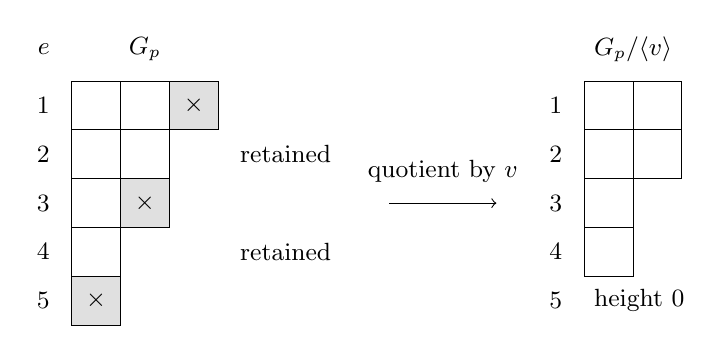
\begin{tikzpicture}[x=0.62cm,y=-0.62cm,
                    every node/.style={font=\small},
                    line width=0.4pt]
 \node at (1.5,-0.65) {\(G_p\)};
 \node[anchor=east] at (-0.25,-0.65) {\(e\)};
 \foreach \e/\k in {1/3,2/2,3/2,4/1,5/1} {
  \node[anchor=east] at (-0.25,{\e-0.5}) {\(\e\)};
  \foreach \i in {1,...,\k} {
   \draw ({\i-1},{\e-1}) rectangle (\i,\e);
  }
 }
 \foreach \e/\i in {1/3,3/2,5/1} {
  \draw[fill=black!12] ({\i-1},{\e-1}) rectangle (\i,\e);
  \node at ({\i-0.5},{\e-0.5}) {\(\times\)};
 }
 \node[anchor=west] at (3.25,1.5) {retained};
 \node[anchor=west] at (3.25,3.5) {retained};
 \draw[->] (6.5,2.5) -- (8.7,2.5);
 \node at (7.6,1.85) {quotient by \(v\)};
 \node at (11.5,-0.65) {\(G_p/\langle v\rangle\)};
 \foreach \e/\k in {1/2,2/2,3/1,4/1} {
  \node[anchor=east] at (10.25,{\e-0.5}) {\(\e\)};
  \foreach \i in {1,...,\k} {
   \draw ({\i+9.5},{\e-1}) rectangle ({\i+10.5},\e);
  }
 }
 \node[anchor=east] at (10.25,4.5) {\(5\)};
 \node[anchor=west] at (10.5,4.5) {height \(0\)};
\end{tikzpicture}

\caption{Layers for \(G_p=\Z/p^5\Z\oplus\Z/p^3\Z\oplus\Z/p\Z\)
and its quotient by \(v=(p^2,p,1)\). The crossed boxes are the layer
drops. Here \((u_1,\ldots,u_5)=(1,1,2,2,3)\), so the retained layers
are \(e=2,4\). On each plateau \(e=2,3\) and \(e=4,5\), retention is
a prefix. The row lengths on the right are the heights of the quotient.}
\label{fig:layers}
\end{figure}

Applied successively to Equation~\eqref{eq:successive-quotients}, this
lemma gives a drop of zero or one at each layer in each quotient. The
same statement applies to the \(h\) successive quotients of \(G_B\)
by the standard basis classes in Equation~\eqref{eq:common-quotient}.
Consequently, for every \((p,e)\),
\begin{equation}\label{eq:common-layer-interlacing}
 k_C(p,e)-h\le k_{H_h}(p,e)\le k_C(p,e),\qquad
 k_B(p,e)-h\le k_{H_h}(p,e)\le k_B(p,e).
\end{equation}
In particular, for \(h=1\) the common height is either \(k_C(p,e)\)
or \(k_C(p,e)-1\), while \(k_B(p,e)\) is either the common height or
one more. This also shows that a layer absent from \(G_C\) has height
at most \(h\) in \(G_B\).

\subsection{The lattice forced by retention}

The next lemma extracts from a set of retained layers a necessary
divisibility condition on the column, with an exact formula for its index.
The condition lies in an
intermediate lattice between \(C\Z^m\) and \(\Z^m\), including when
one preceding column has already been quotiented out.

\begin{lemma}[Retention lattice]\label{lem:retention-lattice}
Let \(C\) be a nonsingular binary matrix of size \(m\), and let
\(\pi:\Z^m\twoheadrightarrow H\) be a quotient map to a finite
abelian group such that \(C\Z^m\subseteq\ker\pi\). Let \(E\) be
any set of positive layers of \(H\). There is a lattice \(K_E\),
depending only on \(\pi,H,E\), with
\begin{equation}\label{eq:retention-lattice}
 C\Z^m\subseteq K_E\subseteq\Z^m,\qquad
 [\Z^m:K_E]=N^{Nq(E)},\qquad
 q(E)=\sum_{(p,e)\in E} k_H(p,e)\nu_p,
\end{equation}
such that the following implication holds for every \(v\in\Z^m\):
if every layer in \(E\) is retained in
\(H\longrightarrow H/\langle\pi(v)\rangle\), then \(v\in K_E\).
\end{lemma}

\begin{proof}
For each prime choose, once for the given group \(H\), cyclic
coordinates
\[
 H_p=\bigoplus_i\Z/p^{b_i}\Z.
\]
Put
\[
 a_{p,i}=\#\{e:(p,e)\in E,\ e\le b_i\},\qquad
 T_E=\bigoplus_{p,i}p^{a_{p,i}}(\Z/p^{b_i}\Z)\subseteq H,
 \qquad K_E=\pi^{-1}(T_E).
\]
Here \(0\le a_{p,i}\le b_i\), and the subgroup in the \((p,i)\)
coordinate consists of the classes divisible by \(p^{a_{p,i}}\).
The lattice \(K_E\) contains \(C\Z^m\). Its index is
\[
 [\Z^m:K_E]=[H:T_E]
 =\prod_{p,i}p^{a_{p,i}}
 =\prod_{(p,e)\in E}p^{k_H(p,e)}
 =N^{Nq(E)},
\]
where the penultimate equality counts a selected layer once for each
cyclic factor reaching it. This proves all assertions about the lattice
and its index.

It remains to prove the implication. Fix \(p,i\), and let \(r_i\) be
the capped valuation of the \(i\)-th coordinate of \(\pi(v)\), as in
the proof of Lemma~\ref{lem:layer-quotient}. Equation~\eqref{eq:quotient-order-exponent}
at \(t=b_i\) gives \(u_{b_i}\ge b_i-r_i\). All the first \(b_i\)
layers are positive, and Equation~\eqref{eq:layer-interlacing} shows
that the number among them that are retained is
\[
 \sum_{e=1}^{b_i}\bigl(1-(u_e-u_{e-1})\bigr)=b_i-u_{b_i}.
\]
If every layer in \(E\) is retained, then
\[
 a_{p,i}\le b_i-u_{b_i}\le r_i.
\]
Thus the coordinate of \(\pi(v)\) is divisible by \(p^{a_{p,i}}\).
This holds in every primary coordinate, so \(\pi(v)\in T_E\) and
\(v\in K_E\), as required.
\end{proof}

For the group in Figure~\ref{fig:layers}, choosing
\(E=\{(p,2),(p,4)\}\) gives divisibility exponents
\((a_{p,1},a_{p,2},a_{p,3})=(2,1,0)\). The two selected layers have
total weight \(2\nu_p\), while \(q(E)=3\nu_p\) and
\([\Z^m:K_E]=p^3\).

For a quotient in Equation~\eqref{eq:successive-quotients}, the map
\(\pi\) is the natural map from \(\Z^m\) onto \(H_{j-1}\).
Conditional on \(C\) and the preceding columns
\(v_1,\ldots,v_{j-1}\), the next column remains uniform on the cube.

\subsection{A symmetric kernel inequality}

The common quotient also controls the destination layers more strongly
than interlacing alone. At a fixed prime \(p\), let \(u_{j,t}\) denote
the exponent from Lemma~\ref{lem:layer-quotient} for
\(H_{j-1}\to H_j\), and set
\begin{equation}\label{eq:total-quotient-loss}
 U_t=\sum_{j=1}^h u_{j,t}
    =F_C(p,t)-F_{H_h}(p,t).
\end{equation}
The equality follows by summing Equation~\eqref{eq:quotient-prefix}.

\begin{lemma}[Symmetric kernel inequality]\label{lem:layer-inequality}
For a nonsingular extension \(B\) of a nonsingular \(C\) of width
\(h\in\{1,2\}\), at every prime \(p\) and every integer \(t\ge0\),
\begin{equation}\label{eq:layer-inequality}
 F_B(p,t)\le F_C(p,t)+ht-2U_t.
\end{equation}
\end{lemma}

\begin{proof}
The assertion is immediate for \(t=0\). Fix \(t\ge1\), put
\(R_t=\Z/p^t\Z\), and reduce the blocks of \(B\) modulo \(p^t\),
writing them as \(C_t,V_t,D_t\). Let
\[
 X=R_t^m,\qquad Y=R_t^h,\qquad
 L=\ker(C_t:X\to X),\qquad J=\im(C_t:X\to X).
\]
The presentation of the cokernel gives
\[
 X/J\cong \Z^m/(C\Z^m+p^t\Z^m)\cong G_C/p^tG_C.
\]
Since \(C_t\) is an endomorphism of the finite group \(X\), its
kernel and cokernel have the same order. Hence
\begin{equation}\label{eq:kernel-prefix-order}
 |L|=|X/J|=p^{F_C(p,t)}.
\end{equation}

Define
\[
 \alpha:Y\longrightarrow X/J,\qquad \alpha(y)=V_ty+J.
\]
The image is the subgroup generated by the column classes in
\(G_C/p^tG_C\). Quotienting by that subgroup gives
\(H_h/p^tH_h\), so Equation~\eqref{eq:total-quotient-loss} gives
\[
 |\im\alpha|=p^{U_t},\qquad |\ker\alpha|=p^{ht-U_t}.
\]
For a kernel vector \((x,y)\in X\oplus Y\) of \(B\) modulo \(p^t\),
the first block equation is
\begin{equation}\label{eq:first-block-kernel}
 C_tx+V_ty=0.
\end{equation}
It requires \(y\in\ker\alpha\). For each such \(y\), its solutions
in \(x\) form a coset \(x_0+L\).

Consider the map
\[
 \gamma:L\longrightarrow Y,\qquad \gamma(z)=V_t^{\mathsf T}z.
\]
We claim that \(|\im\gamma|=p^{U_t}\). Equip \(X\) and \(Y\) with
their standard character pairings, for example
\[
 \langle x,z\rangle_X
   =\exp\!\left(\frac{2\pi i}{p^t}x^{\mathsf T}z\right).
\]
These pairings are perfect: a nonzero coordinate is detected by pairing
with its standard basis vector. For a subgroup \(M\) of either module
\(A\), write \(M^\perp\) for its annihilator. Character orthogonality
gives
\begin{equation}\label{eq:annihilator-order}
 |M|\,|M^\perp|
 =\sum_{a\in A}\sum_{z\in M}\langle a,z\rangle_A
 =|A|.
\end{equation}
For the first equality, the sum over \(M\) is \(|M|\) on its
annihilator and zero elsewhere. For the second, reverse the sums: by
perfectness the sum over \(A\) vanishes for every \(z\ne0\), and the
term \(z=0\) equals \(|A|\).

Symmetry of \(C_t\) gives \(J\subseteq L^\perp\), since
\(\langle C_tx,z\rangle_X=\langle x,C_tz\rangle_X=1\) for
\(z\in L\). Both groups have order \(|X|/|L|\), the former by the
kernel-image formula and the latter by
Equation~\eqref{eq:annihilator-order}. Therefore \(L^\perp=J\).
It follows that
\begin{align*}
 (\im\gamma)^\perp
  &=\{y\in Y:\langle y,V_t^{\mathsf T}z\rangle_Y=1
                    \text{ for every }z\in L\}\\
  &=\{y\in Y:\langle V_ty,z\rangle_X=1
                    \text{ for every }z\in L\}\\
  &=\{y\in Y:V_ty\in J\}=\ker\alpha.
\end{align*}
Equation~\eqref{eq:annihilator-order} in \(Y\) now gives
\[
 |\im\gamma|=\frac{|Y|}{|\ker\alpha|}=p^{U_t},
 \qquad
 |\ker\gamma|=\frac{|L|}{|\im\gamma|}
              =p^{F_C(p,t)-U_t}.
\]

For a fixed \(y\in\ker\alpha\) and \(x=x_0+z\) from
Equation~\eqref{eq:first-block-kernel}, the second block equation is
\[
 \gamma(z)=-V_t^{\mathsf T}x_0-D_ty.
\]
It has either no solutions or one coset of \(\ker\gamma\).
There are at most \(p^{ht-U_t}\) choices for \(y\), and for each at
most \(p^{F_C(p,t)-U_t}\) choices for \(z\). Consequently
\[
 |\ker(B\bmod p^t)|\le p^{F_C(p,t)+ht-2U_t}.
\]
As for \(C_t\), the kernel of the square endomorphism \(B\bmod p^t\)
has the same order as its cokernel. That cokernel is
\(G_B/p^tG_B\), of order \(p^{F_B(p,t)}\). Taking logarithms proves
Equation~\eqref{eq:layer-inequality}.
\end{proof}

Lemma~\ref{lem:retention-lattice} identifies the intermediate lattices
that arise from retaining layers, while Lemma~\ref{lem:layer-inequality}
uses symmetry to relate those retentions to the destination group.
Section~\ref{sec:cube} supplies a uniform bound on cube
intersections with every lattice of the form in
Equation~\eqref{eq:retention-lattice}.

\section{Simultaneous concentration in lattice quotients}\label{sec:cube}

Retaining prescribed layers forces a new bit column into an intermediate
lattice. We now bound the number of bit columns in every coset of every
such lattice, on one typical event for the starting matrix.

Let \(B\) be a nonsingular binary matrix of size \(m\in\mathcal I_N\), and
let
\[
 B\Z^m\subseteq K\subseteq\Z^m.
\]
For \(D\subset[m]\), put
\[
 Q_D=\{z\in\bits^m:z_j=0\text{ for }j\notin D\},\qquad
 M_K(D)=\max_{a\in\Z^m}|Q_D\cap(a+K)|,
 \qquad M_K=M_K([m]).
\]
In particular, \(M_K(D')\le M_K(D)\) whenever \(D'\subset D\).
The lattice \(K\) has full rank, so \(\det K=[\Z^m:K]\). Define
\[
 q=q_K=\frac{\log[\Z^m:K]}{N\log N},
 \qquad\text{so that}\qquad [\Z^m:K]=N^{qN}.
\]
The quotient \(\Z^m/K\) is a quotient of \(G_B\), so
Equation~\eqref{eq:group-order} gives \(0\le q\le1/2\).

For \(0\le d\le1\), write \(f=1-d\) and define
\begin{equation}\label{eq:cube-profile}
 \begin{split}
 c(d/2)&=1-fz(d/f),\\
 z(u)&=
 \begin{cases}
 (1+\sqrt{2u-u^2})^{-1},&0\le u\le1,\\
 1/2,&u\ge1.
 \end{cases}
 \end{split}
\end{equation}
At \(f=0\), the product \(fz(d/f)\) is defined to be zero. Thus
\(c:[0,1/2]\to[0,1]\), with \(c(0)=0\) and \(c(1/2)=1\).

\begin{proposition}[Cube concentration]\label{prop:cube-concentration}
For every fixed \(A>0\), typically for nonsingular binary matrices \(B\)
of size \(m\in\mathcal I_N\), one has simultaneously for every lattice
\(B\Z^m\subseteq K\subseteq\Z^m\)
\begin{equation}\label{eq:cube-concentration}
 M_K\le 2^{N(1-c(q_K)+\ell^{-A})}.
\end{equation}
The typical event may depend on \(A\), but it does not depend on \(K\).
Thus the choice of \(K\) may depend arbitrarily on \(B\) and on any
other data.
\end{proposition}

The function \(c\) is nondecreasing and concave. To see this, put
\(r(u)=\sqrt{2u-u^2}\) for \(0<u<1\). Then
\[
 r'(u)=\frac{1-u}{r(u)},\qquad r''(u)=-\frac1{r(u)^3}.
\]
Consequently \(z=(1+r)^{-1}\) is nonincreasing and convex on \([0,1]\);
more explicitly,
\[
 z''(u)=\frac{1}{r(u)^3(1+r(u))^2}
       +\frac{2(1-u)^2}{r(u)^2(1+r(u))^3}>0.
\]
Its left derivative at \(1\) is zero, so its constant extension remains
convex and nonincreasing. The perspective \(fz(d/f)\) is convex for
\(f>0\): this follows by applying convexity of \(z\) with weights
proportional to the two values of \(f\). Its continuous extension to
the endpoint \(f=0\) is also convex. Restriction to \(f=1-d\) proves
concavity of \(c\). As \(d\) increases, both \(f\) and \(z(d/f)\) are
nonnegative and nonincreasing, which proves monotonicity.

We will use the uniform bound
\begin{equation}\label{eq:cube-holder}
 |c(q)-c(q')|\le C_{\mathrm{pr}}|q-q'|^{1/2}
 \qquad(0\le q,q'\le1/2)
\end{equation}
for an absolute constant \(C_{\mathrm{pr}}\). Indeed, for \(u,v\in[0,1]\),
\[
 |z(u)-z(v)|\le |r(u)-r(v)|
 \le \sqrt{2|u-v|}.
\]
On \(0\le d\le1/2\), the map \(d\mapsto d/(1-d)\) is \(4\)-Lipschitz,
so the product in Equation~\eqref{eq:cube-profile} is
Hölder of exponent \(1/2\) there. On \(1/2\le d\le1\) it is
\((1-d)/2\). Combining the two bounds at \(d=1/2\), and then using
\(d=2q\), gives Equation~\eqref{eq:cube-holder}.

We first count bases of low-height subspaces, and then use that count
to price the witnesses that will arise from a large cube intersection.

\subsection{Low-height bases and witness pricing}

\begin{lemma}[Exact-basis count]\label{lem:exact-basis-count}
Fix \(C,C'>0\). Uniformly for \(m\in\mathcal I_N\) and \(0\le j\le m\),
the number of ordered tuples
\[
 (y,y_1,\ldots,y_j)\in(\bits^m)^{j+1}
\]
for which \(y_1-y,\ldots,y_j-y\) are independent and their span \(W\)
satisfies \(H(W)\le\exp(N\ell^C)\) is at most
\[
 2^{j^2+o(N^2\ell^{-C'})}.
\]
\end{lemma}

\begin{proof}
The case \(j=0\) is immediate. For \(j\ge1\), encode the center \(y\)
and a choice of \(j\) pivot coordinates on which the differences remain
independent. These choices cost \(O(N\log N)\) bits. At the pivots,
each difference entry has two possible values once \(y\) is known, so
all pivot entries cost \(j^2\) bits.

Add the other coordinates in a fixed order. Suppose the current
projected span is \(V\subset\R^h\), and put \(L_V=V\cap\Z^h\). The next
projected span is the graph of a rational functional
\(x\mapsto\langle v,x\rangle\) on \(V\), represented by \(v\in V\). Put
\[
 a=\min\{b\in\Z_{>0}:bv\in L_V^*\}.
\]
The image of \(L_V\) under this functional modulo \(\Z\) has order
\(a\). Hence the projection of the integer lattice in the graph has
index \(a\) in \(L_V\). The volume factor of the graph map on \(V\) is
\(\sqrt{1+\|v\|^2}\), and therefore
\begin{equation}\label{eq:cube-height-ratio}
 \frac{H(\operatorname{graph}(v))}{H(V)}
       =a\sqrt{1+\|v\|^2}.
\end{equation}
All these ratios are at least one. The initial projected space is
\(\R^j\), of height one, and the final one is \(W\). Thus every
intermediate height is at most \(\exp(N\ell^C)\), and a ratio exceeding
\(N^{1/10}\) occurs at most \(O(N\ell^C/\log N)\) times. Mark those
coordinates and encode their \(j\) difference entries directly. Their
total cost is \(O(N^2\ell^C/\log N)\) bits.

At any other coordinate,
\[
 a\le N^{1/10},\qquad \|av\|\le N^{1/10}.
\]
We count possible \(av\) in \(\Lambda=L_V^*\).
Lemma~\ref{lem:normal-height}, applied to \(V\subset\R^h\), gives
\(\det M\ge H(V)^{-1}\) for every sublattice \(M\subset\Lambda\).

Apply Lemma~\ref{lem:det-minimizer} to \(\Lambda\) with
\(T=N^{-1/10}\), choosing a minimizing sublattice as a function of the
known \(V\). If its rank is \(r_0\), comparison with the zero lattice
and the preceding determinant bound give
\[
 H(V)^{-1}\le T^{r_0},\qquad
 r_0\le \frac{10N\ell^C}{\log N}.
\]
Every sublattice of the quotient has determinant at least \(T\) to
its rank. By Lemma~\ref{lem:gaussian-count}, the number of quotient
images of vectors of norm at most \(N^{1/10}\) is
\[
 2^{O(N^{2/5}\log^2N)}.
\]
Here the quotient has rank at most \(N\), and the bound also covers
rank zero.

Encode \(a\), costing \(O(\log N)\) bits, and the quotient image of
\(av\). In a fixed fiber, \(v\) varies in an affine space of dimension
at most \(r_0\). Evaluation on the already known \(j\) independent
projected differences is injective on \(V\), and the evaluations are
the \(j\) entries of the new difference column. Each entry has two
possible values, determined by the corresponding coordinate of \(y\).
An affine space of dimension \(r_0\) meets such a cube in at most
\(2^{r_0}\) points, by projection onto \(r_0\) suitable coordinates.
This bounds the fiber cost by \(r_0\) bits.

Summing over at most \(N\) coordinates, including the pivot, center,
and marking costs, bounds the logarithm of the number of tuples by
\[
 j^2+O\!\left(
   \frac{N^2\ell^C}{\log N}+N^{7/5}\log^2N+N\log N
 \right).
\]
For fixed \(C,C'\), the error is \(o(N^2\ell^{-C'})\), uniformly in
\(j\) and \(m\), as required.
\end{proof}

\begin{proposition}[Witness pricing]\label{prop:witness-pricing}
Fix \(D_0>0\), and put \(\eta=\ell^{-D_0}\) and \(\rho=\eta^3\).
Typically for nonsingular binary matrices \(B\) of size
\(m\in\mathcal I_N\), the following assertion holds simultaneously
for every \(B\Z^m\subseteq K\subseteq\Z^m\).

Let \(S_1,\ldots,S_h\subset\bits^m\) be nonempty subsets, each
\(\rho\)-robust on its affine span, where \(h\le3/\eta\). Suppose
\(S_i-S_i\subset K\), and put \(W_i=\Span(S_i-S_i)\). Suppose also
that \(W=\sum_i W_i\) is a direct sum. Write
\[
 \dim W_i=t_iN,\qquad t=\sum_i t_i,\qquad |S_i|=2^{\alpha_iN}.
\]
If \(D\subset[m]\) has \(|D|=xN\), \(x\le t\), and
\(M_K(D)\le2^{\eta N}\), then
\begin{equation}\label{eq:witness-pricing}
 xt-\frac{x^2}{2}
 \le \sum_i t_i(t_i-\alpha_i)+\eta t+\eta^3.
\end{equation}
\end{proposition}

For a fixed nonsingular matrix \(B\), a \emph{witness} consists of data
\(K,(S_i)_{i=1}^h,D\) satisfying the stated assumptions on the lattice,
sets, their difference spans, and \(D\). It is \emph{violating} if
Equation~\eqref{eq:witness-pricing} fails.
The two sides of that equation have a counting interpretation. In a
symmetric block on \(tN\) coordinates, the number
of independent entries with at least one endpoint in a specified set
of \(xN\) coordinates is
\((xt-x^2/2)N^2+O(N)\). Restricting each row on those coordinates to
at most \(2^{\eta N}\) choices saves this many bits, less
\(\eta tN^2\). For the \(i\)-th set \(S_i\), describing an ordered basis
costs \(t_i^2N^2\) bits to leading order, while robustness supplies
\(\alpha_i t_iN^2\) bits of basis multiplicity. The term
\(t_i(t_i-\alpha_i)\) is the remaining cost. A violation would make
the row saving exceed the total witness cost by \(\eta^3N^2\).

\begin{proof}
The robust-height bound in Lemma~\ref{lem:robust-height}, with the
fixed parameter \(\rho=\ell^{-3D_0}\), gives
\[
 H(W_i)\le\exp(O(N\ell)).
\]
The integer lattice sum of \(W_i\cap\Z^m\) is contained in
\(W\cap\Z^m\). The volume inequality for this sum and saturation give
\[
 H(W)\le\prod_i H(W_i)
       \le\exp(O(N\ell/\eta)).
\]
Choose a fixed \(D_1>D_0+1\). For sufficiently large \(N\), this is at
most \(\exp(N\ell^{D_1})\). We impose
Proposition~\ref{prop:typical-ranks} at this height and at a fixed
precision strong enough that its rank error is at most \(\eta^5N\).
We also impose Proposition~\ref{prop:prime-corank}. Their intersection
is typical. All counting below takes place within this intersection.

For a fixed list of dimensions, Lemma~\ref{lem:exact-basis-count}
counts centers and ordered bases of differences for the pieces with
total logarithmic cost
\begin{equation}\label{eq:witness-basis-upper}
 N^2\sum_i t_i^2+o(N^2\eta^4).
\end{equation}
Indeed, use that Lemma with a fixed \(C'\) larger than \(5D_0\) and
sum its errors over at most \(3/\eta\) pieces. The height exponent
there can be chosen fixed and large enough for all the \(W_i\).

For each individual witness, fix a center in each \(S_i\). At every
stage of choosing an ordered basis of differences, the affine span of
the center and the points already chosen is a proper affine
subspace of \(\aff S_i\). Robustness bounds the fraction of \(S_i\)
in that subspace by \(2^{-\rho}\). Consequently the number of choices
of an ordered basis for this piece is at least
\[
 \bigl((1-2^{-\rho})\,2^{\alpha_iN}\bigr)^{t_iN}.
\]
The choices for different pieces form distinct basis lists. As
\(t\le m/N\le1\), their total logarithm is at least
\begin{equation}\label{eq:witness-basis-lower}
 N^2\sum_i t_i\alpha_i
       -O\bigl(N\log(1/\rho)\bigr)
 =N^2\sum_i t_i\alpha_i-o(N^2\eta^4).
\end{equation}

Fix basis-list data, so in particular \(W\) is known. For a witnessed
matrix choose a coordinate set \(Y_0\) of size \(tN\) containing \(D\).
The second rank assertion of Proposition~\ref{prop:typical-ranks}
shows that the columns on \([m]\setminus Y_0\), projected off \(W\),
have rank at least \(m-tN-\eta^5N\). Choose an independent collection
there, and use nonsingularity of \(B\) to complete it to a basis of
the quotient \(\R^m/W\) using columns of \(B\). Let \(P\) be the
resulting set of \(m-tN\) indices and \(Y=[m]\setminus P\). Then
\[
 |D\cap P|\le\eta^5N.
\]
Encode \(D\) and \(P\), at cost \(O(N)\) bits, and reveal the columns
on \(P\). If \(T_m=m(m+1)/2\) is the total number of independent bits
of \(B\), these columns cost
\[
 T_m-\binom{tN+1}{2}
\]
bits, using symmetry.

The revealed columns and the basis differences are \(m\) independent
integer vectors: the differences form a basis of \(W\), and the
revealed columns project to a basis off \(W\). Let \(L\) be their
integer span. It is known from the encoded data, satisfies
\(L\subset K\), and has full rank. Each generating vector has norm
at most \(\sqrt N\), so Hadamard's inequality gives
\[
 |\Z^m/L|\le N^{m/2}\le N^{N/2}.
\]
We next enumerate the possible \(K\) containing this known \(L\).
Let \(r_N=\lceil N^{3/5}\rceil\). For every prime \(p\),
\[
 \dim_{\F_p}\bigl((\Z^m/K)/p(\Z^m/K)\bigr)
 \le\dim_{\F_p}(G_B/pG_B)
 =\corank_{\F_p}B\le r_N
\]
by Proposition~\ref{prop:prime-corank}. The minimum number of
generators of a finite abelian group is the maximum of these
dimensions over its primes, as follows from its invariant factors.
Thus \(\Z^m/K\), and also its character dual, can be generated by at most
\(r_N\) elements.

Put \(H=\Z^m/L\). The annihilator of \(K/L\) identifies
\((\Z^m/K)^\vee\) with a subgroup of
\(H^\vee=\Hom(H,\mathbb Q/\Z)\); by finite duality this subgroup determines
\(K\). Every subgroup with at most
\(r_N\) generators is generated by some ordered \(r_N\)-tuple in
\(H^\vee\), padding with zero elements if necessary. The number of
possible \(K\) is therefore at most \(|H|^{r_N}\). Its logarithm is
\begin{equation}\label{eq:witness-lattice-cost}
 O(N^{8/5}\log N)=o(N^2\eta^4).
\end{equation}
This candidate list is formed after the basis lists and revealed
columns fix \(L\), before the remaining matrix block is encoded.
It may include lattices incompatible with every completion. The
prime-corank condition is used only to ensure that each actual
witnessed \(K\) appears in the list.

Write \(D'=D\cap Y\), \(y=|Y|=tN\), and \(d'=|D'|\). We have
\(d'\ge(x-\eta^5)N\) and \(M_K(D')\le M_K(D)\le2^{\eta N}\). In the
remaining \(Y\)-block, first encode the symmetric bits on
\(Y\setminus D'\), at cost \(\binom{y-d'+1}{2}\). For a row indexed
by \(Y\setminus D'\), all entries outside \(D'\) are now known.
The full row belongs to \(K\), since \(B\) is symmetric and each
column belongs to \(B\Z^m\). Its entries on \(D'\) therefore lie in a
fixed coset of \(K\) and have at most \(M_K(D')\) possibilities.
This encodes the cross block at cost at most \(\eta N(y-d')\).
For the final \(D'\)-block, the same bound applies to each of its
\(d'\) rows. Ignoring symmetry within that block only enlarges the
count, so its cost is at most \(\eta Nd'\). Relative to an unrestricted
symmetric \(Y\)-block the saving is at least
\[
 \begin{split}
 \binom{y+1}{2}-\binom{y-d'+1}{2}-\eta Ny
 &=yd'-\frac{(d')^2}{2}+\frac{d'}2-\eta Ny\\
 &\ge N^2\left(xt-\frac{x^2}{2}-\eta t
                  -O(\eta^5+1/N)\right).
 \end{split}
\]

It remains to compare the upper count with the multiplicity of
witnesses. Group violating witnesses by \(h\), the integers \(t_iN\)
and \(xN\), and the integers
\[
 a_i=\lfloor\log_2|S_i|\rfloor,\qquad \bar\alpha_i=a_i/N.
\]
There are at most \(2^{O(\eta^{-1}\log N)}\) groups. Fix one group,
and let \(\mathcal E\) be the set of matrices in the imposed typical
intersection that have a violating witness in this group. For each
\(B\in\mathcal E\), select one such witness and count the distinct
pairs consisting of \(B\) and the basis lists supplied by that
witness. Equation~\eqref{eq:witness-basis-lower} gives a lower bound
of
\[
 |\mathcal E|\,
 2^{N^2\sum_i t_i\bar\alpha_i-o(N^2\eta^4)}
\]
on the number of pairs. On the other hand,
Equations~\eqref{eq:witness-basis-upper} and
\eqref{eq:witness-lattice-cost}, together with the matrix saving,
give the upper bound
\[
 2^{T_m+
 N^2\left(\sum_i t_i^2-xt+x^2/2+\eta t\right)
 +o(N^2\eta^4)}.
\]
The enumeration may count a pair more than once if it has several
compatible choices of \(D,P,K\); this preserves the upper bound.
In particular, the lower bound selects just one witness per matrix,
while the upper bound includes the union over all \(K\).

Since \(0\le\alpha_i-\bar\alpha_i<1/N\) and \(t\le1\), violation of
Equation~\eqref{eq:witness-pricing} implies
\[
 \sum_i t_i(t_i-\bar\alpha_i)-xt+x^2/2+\eta t
 <-\eta^3+\frac1N.
\]
All binary matrices have probability \(2^{-T_m}\). Dividing the pair
bounds therefore gives
\[
 \Pr(\mathbf B_m\in\mathcal E)
 \le 2^{-N^2\eta^3+o(N^2\eta^4)}.
\]
The group count and all omitted costs are absorbed in this error.
Since \(N\eta^3\to\infty\), the total probability of a violation is
\(2^{-\omega(N)}\), including the exceptional probabilities of the
imposed rank and corank properties. This proves the assertion, including its
simultaneity over the lattices, lists, and coordinate sets.
\end{proof}

\subsection{From witness pricing to concentration}

\begin{proof}[Proof of Proposition~\ref{prop:cube-concentration}]
Fix \(A>0\). Choose a fixed \(D_0>2A\), and put
\(\eta=\ell^{-D_0}\), \(\rho=\eta^3\). Work on the
typical event in Proposition~\ref{prop:witness-pricing}, and fix an
arbitrary \(K\) with \(B\Z^m\subseteq K\subseteq\Z^m\).

Apply Lemma~\ref{lem:det-minimizer} to \(K\) with
\(T=(\log N)^4\), and let \(K_0\) be a minimizing saturated sublattice.
Put \(F=\Span K_0\) and
\[
 d=\frac{m-\dim F}{N},\qquad
 f=1-d=\frac{\dim F+N-m}{N}.
\]
The projected quotient \(K/K_0\) has rank \(dN\) and all its
sublattices have determinant at least \(T\) to their rank. Moreover
\(\det K_0\le T^{\dim F}\), by comparison with the zero lattice.
The projections of the columns of \(B\) span \(F^\perp\), and each
has norm at most \(\sqrt N\). Choosing \(dN\) independent projections
and using that their integer span is a sublattice of \(K/K_0\) gives
\(\det(K/K_0)\le N^{dN/2}\). Hence
\begin{equation}\label{eq:cube-order-dimension}
 q=\frac{\log\det K}{N\log N}
 \le \frac d2+\frac{\dim F}{N}\frac{\log T}{\log N}
 \le \frac d2+\frac{4\ell}{\log N}.
\end{equation}

Consider any nonempty subset \(S\) of a coset of \(K\) in the cube, and base
its differences at one point of \(S\). Their projections off \(F\)
belong to \(K/K_0\) and have norm at most \(\sqrt N\).
Lemma~\ref{lem:gaussian-count} gives at most
\[
 2^{O(N/\log^6N)}
\]
distinct projections. Restrict to a largest projection fiber and
then apply Lemma~\ref{lem:robust-extraction} with parameter
\(\rho=\eta^3\). For sufficiently large \(N\), these two operations
lose at most \(2\eta^3N\) bits of logarithmic size. Thus, if
\(|S|=2^{aN}\), they give a \(\rho\)-robust subset \(S'\) with
\begin{equation}\label{eq:cube-fiber-extraction}
 |S'|\ge2^{(a-2\eta^3)N},
 \qquad \Span(S'-S')\subset F.
\end{equation}
If \(S\) is supported on a coordinate set, the same is true of its
differences after these operations.

Choose a set \(P_F\) of \(\dim F\) pivot coordinates for \(F\), so
coordinate projection onto \(P_F\) is injective on \(F\), and put
\(J_0=[m]\setminus P_F\). Then \(|J_0|=dN\) and a vector supported on
\(J_0\) belongs to \(F\) only if it is zero. Distinct bit vectors
supported on \(J_0\) therefore have distinct projections off \(F\):
equal projections would give a difference in \(F\). Applying the
preceding projection count to a coset intersection on \(J_0\) gives
\begin{equation}\label{eq:cube-pivot-complement}
 M_K(J_0)\le2^{O(N/\log^6N)}\le2^{\eta N}.
\end{equation}

Write \(M_K=2^{\alpha N}\). We have \(0\le\alpha\le1\). If
\(\alpha<10\eta\), the conclusion follows for sufficiently large
\(N\), since \(1-c(q)\ge0\) and \(10\eta\le\ell^{-A}\). We may
therefore assume \(\alpha\ge10\eta\).

Apply Equation~\eqref{eq:cube-fiber-extraction} to a full-coordinate
coset attaining \(M_K\). Denote the resulting robust subset by \(S_*\),
put \(W_*=\Span(S_*-S_*)\), and write
\[
 |S_*|=2^{\alpha_*N},\qquad v=\frac{\dim W_*}{N}.
\]
An affine space of dimension \(\dim W_*\) contains at most
\(2^{\dim W_*}\) cube points, by coordinate projection. Consequently
\begin{equation}\label{eq:cube-full-witness}
 \alpha_*\ge\alpha-2\eta^3,\qquad
 \alpha-2\eta^3\le v\le\frac{\dim F}{N}\le f.
\end{equation}
The last inequality uses \(m\le N\).

We construct one coordinate set \(D\) with small \(M_K(D)\) and use it
in two applications of Proposition~\ref{prop:witness-pricing}. A list of
robust sets will force \(D\) to be large; applying the estimate to the
full-coordinate set \(S_*\) then restricts how large \(\alpha\) can be
for that same \(D\).

Initially all coordinates of \(P_F\) are available. At step \(i\),
choose, among the available coordinates, a set \(A_i\) of
\emph{minimum cardinality} such that
\[
 M_K(J_0\cup A_i)>2^{\eta N}.
\]
For a coset attaining \(M_K(J_0\cup A_i)\), apply
Equation~\eqref{eq:cube-fiber-extraction}. It gives a robust subset
\(S_i\) whose difference span satisfies
\[
 W_i\subset F\cap E_{J_0\cup A_i},\qquad
 \alpha_i=\frac{\log_2|S_i|}{N}\ge\eta-2\eta^3,\qquad
 t_i=\frac{\dim W_i}{N}\ge\alpha_i.
\]
Because projection of \(F\) onto \(P_F\) is injective and \(W_i\)
vanishes on \(P_F\setminus A_i\), we have \(t_iN\le|A_i|\). Choose
\(t_iN\) pivot coordinates \(H_i\subset A_i\) on which projection of
\(W_i\) is injective, and declare those coordinates unavailable.
Stop when \(t=\sum_i t_i\ge\alpha-2\eta\).

The required set \(A_i\) exists before the stopping condition is met.
Indeed, the coordinates already declared unavailable number \(tN\).
In a full coset attaining \(M_K\), fix their bit values to a most
frequent pattern. At least \(2^{(\alpha-t)N}>2^{2\eta N}\) points
remain. Subtracting the fixed pattern on those coordinates translates
the coset and leaves bit vectors supported on \(J_0\) and the available
coordinates. Hence that coordinate set has \(M_K>2^{\eta N}\).
Equation~\eqref{eq:cube-pivot-complement} also shows that each \(A_i\)
is nonempty.

The spaces \(W_i\) form a direct sum. In a relation \(\sum_i w_i=0\)
with \(w_i\in W_i\), the later terms vanish on the pivots \(H_1\);
injectivity on \(W_1\) gives \(w_1=0\), and the same argument
successively gives every \(w_i=0\). Thus \(t\le\dim F/N\le1\).
Each increment is at least \(\eta-2\eta^3\), so there are fewer than
\(3/\eta\) steps for sufficiently large \(N\). Together with the
existence just proved, this ensures that the stopping condition is
reached. The family of available subsets only shrinks from one step
to the next. Since each \(A_i\) has minimum cardinality, the numbers
\(|A_i|\) do not decrease. If the last one has size \(sN\), then
\begin{equation}\label{eq:cube-coordinate-list}
 t\ge\alpha-2\eta,\qquad t_i\le |A_i|/N\le s
 \quad\text{for every }i.
\end{equation}

Remove one coordinate from the last \(A_i\) and include all of \(J_0\).
The resulting set \(D\) satisfies
\begin{equation}\label{eq:cube-small-coordinate-set}
 |D|=(d+s)N-1,\qquad M_K(D)\le2^{\eta N},
\end{equation}
by the minimum cardinality of that \(A_i\). For \(x\ge0\), \(t>0\),
define
\[
 e(x,t)=
 \begin{cases}
 x-x^2/(2t),&0\le x\le t,\\
 t/2,&x\ge t.
 \end{cases}
\]
This function is nondecreasing in both variables. Its rate of change
in \(x\) is between zero and one, and its rate of change in \(t\) is
between zero and \(1/2\). These assertions follow from
\[
 \partial_x e=1-x/t,\quad \partial_t e=x^2/(2t^2)\quad(x<t),
 \qquad
 \partial_x e=0,\quad \partial_t e=1/2\quad(x>t),
\]
and continuity at \(x=t\).

If necessary, truncate \(D\) to a subset of size \(tN\).
Monotonicity of \(M_K(D)\) preserves its bound, so
Proposition~\ref{prop:witness-pricing} applied to the constructed list
gives
\[
 \begin{split}
 e(d+s,t)
 &\le \frac1t\sum_i t_i(t_i-\alpha_i)
       +\eta+\frac{\eta^3}{t}+\frac1N\\
 &\le s+O(\eta).
 \end{split}
\]
The \(1/N\) accounts for the coordinate removed in
Equation~\eqref{eq:cube-small-coordinate-set}. The last inequality
uses \(\alpha_i\ge0\), \(t_i\le s\), and
\(t\ge\alpha-2\eta\ge8\eta\). Replacing \(t\) by \(\alpha\) keeps
this bound: if \(t\ge\alpha\), use monotonicity in the second
variable; if \(t<\alpha\), use its \(1/2\)-Lipschitz bound and
\(\alpha-t\le2\eta\). Thus \(e(d+s,\alpha)\le s+O(\eta)\).

Put \(h=d+s\). If \(h\le\alpha\), the last inequality gives
\[
 d\le \frac{h^2}{2\alpha}+O(\eta).
\]
Since \(\alpha\le1\), it follows that
\(h\ge\sqrt{2d\alpha}-O(\sqrt\eta)\). If \(h\ge\alpha\), it instead
gives \(s\ge\alpha/2-O(\eta)\), and then
\[
 h\ge d+\alpha/2-O(\eta)
   \ge\sqrt{2d\alpha}-O(\eta).
\]
We have proved
\begin{equation}\label{eq:cube-coordinate-lower}
 d+s\ge\sqrt{2d\alpha}-O(\sqrt\eta).
\end{equation}

Use the same \(D\) again, now with the singleton list consisting of
\(S_*\). Truncate \(D\) to size \(vN\) if necessary. From
Proposition~\ref{prop:witness-pricing} and
Equation~\eqref{eq:cube-full-witness},
\[
 e(d+s,v)
 \le v-\alpha_*+\eta+\frac{\eta^3}{v}+\frac1N
 \le v-\alpha+O(\eta).
\]
Here \(v\ge\alpha-2\eta^3\ge9\eta\) for large \(N\). Since \(v\le f\)
and the rate of change of \(e\) in its second argument is at most
\(1/2\), this yields
\begin{equation}\label{eq:cube-coordinate-upper}
 e(d+s,f)
 \le e(d+s,v)+\frac{f-v}{2}
 \le f-\alpha+O(\eta).
\end{equation}

We finish by solving the two coordinate inequalities. In the present
case \(f\ge v>0\). If \(d\ge f\), then \(d+s\ge f\), so
Equation~\eqref{eq:cube-coordinate-upper} gives
\[
 \alpha\le f/2+O(\eta)=fz(d/f)+O(\eta).
\]
Suppose instead that \(d\le f\). Monotonicity and the unit Lipschitz
bound of \(e\) in its first argument, together with
Equations~\eqref{eq:cube-coordinate-lower} and
\eqref{eq:cube-coordinate-upper}, give
\begin{equation}\label{eq:cube-profile-inequality}
 e(\sqrt{2d\alpha},f)\le f-\alpha+O(\sqrt\eta).
\end{equation}
Put \(u=d/f\in[0,1]\). Directly from
Equation~\eqref{eq:cube-profile},
\[
 2uz(u)\le1,\qquad
 1-z(u)=\sqrt{2uz(u)}-uz(u).
\]
For completeness, if \(r=\sqrt{2u-u^2}\), then
\((1-u)^2z(u)^2-2z(u)+1=0\), which gives the second identity after
taking the nonnegative square root. The first is equivalent to
\(2u\le1+r\); for \(u\le1/2\) it is immediate, and for
\(u\ge1/2\) its square follows from
\(r^2-(2u-1)^2=(1-u)(5u-1)\ge0\). These identities show that
\(\alpha_0=fz(u)\) satisfies
\[
 e(\sqrt{2d\alpha_0},f)=f-\alpha_0.
\]
The function \(a\mapsto a+e(\sqrt{2da},f)\) is nondecreasing and
increases by at least the increase in \(a\). Therefore
Equation~\eqref{eq:cube-profile-inequality} implies
\(\alpha\le\alpha_0+O(\sqrt\eta)\). Both cases give
\[
 \alpha\le fz(d/f)+O(\sqrt\eta)
          =1-c(d/2)+O(\sqrt\eta).
\]

By Equation~\eqref{eq:cube-order-dimension}, monotonicity of \(c\),
and Equation~\eqref{eq:cube-holder},
\[
 c(q)\le c(d/2)+O\!\left(\sqrt{\frac{\ell}{\log N}}\right).
\]
It follows that
\[
 \alpha\le 1-c(q)+O(\sqrt\eta)
                    +O\!\left(\sqrt{\frac{\ell}{\log N}}\right).
\]
Because \(D_0>2A\) is fixed, both error terms are
\(o(\ell^{-A})\). Increasing \(N\) makes their sum at most
\(\ell^{-A}\), proving Equation~\eqref{eq:cube-concentration}.
The argument was deterministic for every \(K\) on the single typical
event of Proposition~\ref{prop:witness-pricing}, so the conclusion
is simultaneous in \(K\).
\end{proof}

\section{Pricing retained layers by certificates}\label{sec:certificate-pricing}

Retaining layers in a quotient imposes a lattice condition on the new
column. We now count partial certificates of that condition. The resulting
estimate permits the certificate size to be chosen separately in each
class of outcomes; this will allow a later argument to choose it according
to the largest potential in that class.

We first record the probability bound for a fixed certificate at any
fixed cube precision \(A_{\mathrm{cube}}>0\). Let \(\mathcal F\) be exposed
information that fixes a nonsingular binary matrix \(C\) of size
\(m\in\mathcal I_N\) and a quotient map
\(\pi:\Z^m\twoheadrightarrow G\) with \(C\Z^m\subseteq\ker\pi\).
Suppose that, conditionally on \(\mathcal F\), a column \(v\) is uniform
on \(\bits^m\). Take \(C\) in the typical set of
Proposition~\ref{prop:cube-concentration} at precision
\(A_{\mathrm{cube}}\).

Fix a candidate set \(E\) of positive layers of \(G\) after these data
are fixed, and let \(\mathcal R\) be the layers retained on quotienting
\(G\) by \(\pi(v)\). Lemma~\ref{lem:retention-lattice} gives a lattice
\(K_E\), fixed by \(\pi\) and \(E\), such that \(E\subseteq\mathcal R\)
implies \(v\in K_E\), with
\[
 C\Z^m\subseteq K_E\subseteq\Z^m,\qquad
 [\Z^m:K_E]=N^{Nq(E)},\qquad
 q(E)=\sum_{(p,e)\in E}k_G(p,e)\nu_p.
\]
The group-order bound in Equation~\eqref{eq:group-order} gives
\(0\le q(E)\le1/2\). Conditional uniformity of \(v\) and the
simultaneous cube estimate therefore give
\begin{equation}\label{eq:fixed-certificate-probability}
 \begin{aligned}
 \Pr(E\subseteq\mathcal R\mid\mathcal F)
 &\le \Pr(v\in K_E\mid\mathcal F)
 \le 2^{-m}M_{K_E}\\
 &\le 2^{-m}2^{N(1-c(q(E))+\ell^{-A_{\mathrm{cube}}})}
 =2^{-N(c(q(E))-\eta_N)},\\
 \eta_N&=\ell^{-A_{\mathrm{cube}}}+1-\frac mN.
 \end{aligned}
\end{equation}
Here \(1-m/N\le N^{-3/10}\). The same typical set works for every
exposed quotient, since all its certificate lattices contain the original
\(C\Z^m\).
We will handle marks that depend on \(v\) by counting the fixed candidates
and how many each outcome offers.

For \(0\le t\le1\), let
\[
 H_2(t)=-t\log_2t-(1-t)\log_2(1-t),
 \qquad H_2(0)=H_2(1)=0.
\]
For \(s,u\ge0\) and \(0\le x\le s\), define
\begin{equation}\label{eq:entropy-cost}
 \mathcal E(s,u,x)
 =(s+u)H_2\!\left(\frac{x}{s+u}\right)
       -sH_2\!\left(\frac{x}{s}\right),
\end{equation}
using the continuous values when a denominator vanishes. Here \(s\) and
\(u\) will be the total weights of marked and unmarked layers, and \(x\)
will be a target weight for a certificate chosen among the marked layers.
When all layers have weight \(1/N\), the ratio
\(\binom{(s+u)N}{xN}/\binom{sN}{xN}\) counts possible certificates
relative to those offered by a fixed marked set, and its base-two logarithm
is \(N\mathcal E(s,u,x)+O(\log N)\) for integer counts.

\begin{proposition}[Certificate pricing]\label{prop:certificate-pricing}
Fix \(A>0\) and at most two positive constants \(w_i\). Typically for
nonsingular binary matrices \(C\) of size
\(m\in\mathcal I_N\), the following assertion holds. The typical set
is obtained by imposing Proposition~\ref{prop:cube-concentration} at a
sufficiently large fixed precision depending on \(A\) and these constants.

Let \(\mathcal F\) denote exposed information which fixes \(C\), a
quotient map \(G_C\twoheadrightarrow G\), and the data described next.
Suppose that, conditionally on \(\mathcal F\), a tested column \(v\) is
uniform on \(\bits^m\). Partition the layers of \(G\) into at most two
categories, each a union of whole plateaus. In category \(i\), assume
that every height is at least \(w_i\); only \(w_i=1,2\) will be needed.
The partition is part of the exposed data. In the quotient of \(G\) by the image of \(v\),
an outcome may mark some of the retained layers. Require that the marked
layers on each plateau form a prefix. The marks may also depend on other
random bits in the experiment.

Let \(\mathcal A\) be any subevent of this experiment. There is a
partition of \(\mathcal A\) into at most \(2^{N\ell^{-A}}\) classes,
constructed before choosing a representative or any target weights, with
the following property. Take any nonempty class \(\mathcal A_\alpha\),
any representative outcome in it, and write \(s_i\) and \(u_i\) for
the representative's sums of the weights \(\nu_p\) of the marked and
unmarked layers in category \(i\). For any choices \(0\le x_i\le s_i\),
\begin{equation}\label{eq:certificate-pricing}
 \Pr(\mathcal A_\alpha\mid\mathcal F)
 \le 2^{-N\left(
 c\left(\sum_i w_i x_i\right)
       -\sum_i\mathcal E(s_i,u_i,x_i)-\ell^{-A}\right)}.
\end{equation}
Here \(\mathcal A_\alpha\) already includes the restriction to
\(\mathcal A\); the probability is conditioned only on the exposed
information. The class count and the estimate are uniform in that
information, the quotient, the subevent, and the representative. In
particular, the exposed information may include a preceding column that
fixes \(G\), provided the tested column remains conditionally uniform.
\end{proposition}

We record the entropy facts needed below. Put
\[
 H(s,u)=(s+u)H_2\!\left(\frac{s}{s+u}\right),\qquad H(0,0)=0.
\]
Expansion of the logarithms gives
\begin{equation}\label{eq:entropy-difference}
 \mathcal E(s,u,x)=H(s,u)-H(s-x,u).
\end{equation}
For \(s>0\),
\[
 \frac{\partial H}{\partial s}(s,u)=\log_2(1+u/s),
\]
which is nonnegative and nonincreasing in \(s\). Thus \(\mathcal E\ge0\).
For fixed \(s,u\), the function \(\mathcal E(s,u,x)\) is convex in
\(x\in[0,s]\): in the interior its derivative is
\(\log_2(1+u/(s-x))\), which is nondecreasing in \(x\). For fixed
\(u,x\), it is nonincreasing in \(s\ge x\), since for \(s>x\),
\[
 \frac{\partial\mathcal E}{\partial s}(s,u,x)
 =\log_2(1+u/s)-\log_2(1+u/(s-x))\le0.
\]
The endpoint cases follow by continuity. The defining formula also gives
homogeneity of degree one in all three size variables:
\(\mathcal E(ts,tu,tx)=t\mathcal E(s,u,x)\) for \(t\ge0\).
For fixed \(0\le\theta\le1\), write
\[
 \mathcal E_\theta(s,u)=\mathcal E(s,u,\theta s).
\]
This function is concave and homogeneous of degree one in \((s,u)\).
Indeed, the first term in
\[
 \mathcal E_\theta(s,u)
 =(s+u)H_2\!\left(\frac{\theta s}{s+u}\right)-sH_2(\theta)
\]
is the perspective of the concave function \(H_2\), composed with a
linear map, and the second term is linear. Consequently
\(\mathcal E_\theta\) is superadditive on the nonnegative quadrant:
\begin{equation}\label{eq:entropy-superadditive}
 \sum_j\mathcal E_\theta(s_j,u_j)
 \le \mathcal E_\theta\!\left(\sum_j s_j,\sum_j u_j\right).
\end{equation}

These functions have uniform continuity estimates at their boundaries.
For every fixed \(M\), the function \(-t\log_2t\), extended by zero at
zero, is H\"older continuous of exponent \(1/2\) on \([0,M]\). To see
this, integrate its derivative on an interval of length \(d\); the
absolute integral is at most
\(O_M(d(1+|\log d|))=O_M(\sqrt d)\), with the same conclusion for
intervals meeting zero. Expressing \(H(s,u)\) as
\[
 -s\log_2s-u\log_2u+(s+u)\log_2(s+u)
\]
therefore shows that it is H\"older continuous of exponent \(1/2\) on
every bounded nonnegative rectangle. Equation~\eqref{eq:entropy-difference}
gives the same estimate for \(\mathcal E(s,u,x)\) on bounded parts of
its domain. It also gives an estimate for \(\mathcal E_\theta(s,u)\)
whose constant is uniform over \(0\le\theta\le1\). We will use these
estimates both to round certificate cardinalities and to replace layer
weights by nearby cell weights.

\begin{proof}
Work conditionally on fixed exposed data satisfying the assumptions.
Choose a fixed cube precision \(A_{\mathrm{cube}}>0\), to be specified at
the end, and invoke Equation~\eqref{eq:fixed-certificate-probability} for
each fixed candidate \(E\). Here the quotient map
\(G_C\twoheadrightarrow G\), composed with the natural map from \(\Z^m\),
gives the exposed map \(\pi\) in that observation. This uses only the
conditional uniformity of \(v\); additional random bits and the restriction
to \(\mathcal A\) need not be independent of \(v\).

We now construct the classes. Fix a large constant \(D>0\), to be
chosen at the end, and set \(\delta=\ell^{-D}\) and
\(a_p=\log_Np\). The order bound gives
\begin{equation}\label{eq:certificate-order-bounds}
 \sum_{p,e}k_G(p,e)\frac{a_p}{N}\le\frac12,
 \qquad
 \sum_{p,e}k_G(p,e)\le\frac{N\log N}{2\log2}.
\end{equation}
We classify the marks in three prime ranges.

For \(a_p>\ell^D\), record every mark bit. There are at most
\(N/(2\ell^D)\) layers in this range by the first bound in
Equation~\eqref{eq:certificate-order-bounds}, so this record costs
\(O(N\ell^{-D})\) bits.

For \(a_p<1-\delta\), record the number of marks on each plateau.
These counts determine all the marks because they are prefixes.
There are at most \(N^{1-\delta}\) primes in this range. If \(d_p\)
is the number of plateaus at \(p\), their distinct positive heights
give
\[
 \frac{d_p(d_p+1)}2\le\sum_e k_G(p,e).
\]
Cauchy--Schwarz and the second bound in
Equation~\eqref{eq:certificate-order-bounds} show that the total number
of these plateaus is
\(O(N^{1-\delta/2}\sqrt{\log N})\). Each prefix count costs
\(O(\log N)\) bits, since every plateau length is \(O(N\log N)\).
The total cost is therefore
\[
 O\!\left(N^{1-\delta/2}(\log N)^{3/2}\right)
       =o(N\ell^{-D}).
\]
For the last equality, use
\(\delta\log N=(\log N)/\ell^D\gg\log\log N\).

The remaining primes satisfy \(1-\delta\le a_p\le\ell^D\).
For each category, split this range into bins of width at most
\(\delta\), starting at \(1-\delta\), and call a category-bin pair
a cell. There are \(J=O(\ell^{2D})\) cells. In a cell \(j\), let
\(\lambda_j\) be the lower endpoint of its bin, so
\[
 1-\delta\le\lambda_j\le\ell^D,
 \qquad \lambda_j\le a_p\le\lambda_j+\delta
 \quad\hbox{for its layers}.
\]
The number of layers in this entire range is \(O(N)\), again by the
first order bound. Record only the number of marks in each cell. This
costs \(O(\ell^{2D}\log N)=o(N\ell^{-D})\) bits. All these records
depend only on the marks and the exposed data; intersecting their classes
with \(\mathcal A\) gives the desired classes for the subevent. Their
number is at most \(2^{O(N\ell^{-D})+o(N\ell^{-D})}\), uniformly in
the exposed quotient.

Fix one class, a representative, and target weights as in the statement.
For category \(i\), put \(\theta_i=x_i/s_i\) if \(s_i>0\), and put
\(\theta_i=0\) otherwise. In the large and small prime ranges the
marked sets are known throughout the class; include all of them in each
certificate. In an intermediate cell \(j\) of category \(i\), let
\(n_j\) be its number of layers and \(r_j\) its recorded number of
marks, and require a certificate to contain any
\[
 a_j=\lfloor\theta_i r_j\rfloor
\]
of those marked layers. Thus every outcome in the class offers exactly
\[
 \mathfrak m=\prod_j\binom{r_j}{a_j}
\]
certificates, whereas the number of possible certificates for the class
is at most
\[
 \mathfrak n=\prod_j\binom{n_j}{a_j}.
\]
Empty products have value one. The latter count is an upper bound because
it allows arbitrary layers in each cell, without imposing the prefix
restriction.

We check the weight certified by each such choice uniformly over all
outcomes in the class. In category \(i\), let \(s_i^0\) be the marked
weight in the large and small prime ranges; it is fixed in the class.
The representative's marked weight in its intermediate cells differs
from \(\sum_{j\in i}\lambda_jr_j/N\) by at most
\(\delta\sum_{j\in i}r_j/N=O(\delta)\). The weight selected in those
cells is at least
\[
 \sum_{j\in i}\frac{\lambda_j a_j}{N}
 \ge \theta_i\sum_{j\in i}\frac{\lambda_j r_j}{N}
              -\frac1N\sum_{j\in i}\lambda_j.
\]
The last term is \(O(\ell^{3D}/N)=o(\delta)\). Since all of the
known marked weight is included and \(s_i^0\ge\theta_i s_i^0\), the
selected weight in this category is at least \(x_i-O(\delta)\).
Every selected layer there has height at least \(w_i\). Consequently,
uniformly over its choices,
\begin{equation}\label{eq:certificate-index-lower-bound}
 q(E)\ge q_0-O(\delta),\qquad q_0=\sum_i w_i x_i.
\end{equation}
Both \(q(E)\) and \(q_0\) belong to \([0,1/2]\): for the latter,
\(q_0\le\sum_i w_i s_i\le\sum_{p,e}k_G(p,e)\nu_p\).
The profile \(c\) is increasing and H\"older continuous of exponent
\(1/2\) on this interval. Equation~\eqref{eq:certificate-index-lower-bound}
therefore gives
\[
 c(q(E))\ge c(q_0)-O(\sqrt\delta).
\]
Together with Equation~\eqref{eq:fixed-certificate-probability}, this
bounds the probability of offering any one fixed candidate certificate
by \(2^{-N(c(q_0)-\eta_N-O(\sqrt\delta))}\). This conclusion holds
after intersection with the class and with \(\mathcal A\), since such
an intersection still implies \(v\in K_E\).

Double counting outcome-certificate pairs now yields
\begin{equation}\label{eq:certificate-double-count}
 \Pr(\mathcal A_\alpha\mid\mathcal F)
 \le \frac{\mathfrak n}{\mathfrak m}
       2^{-N(c(q_0)-\eta_N-O(\sqrt\delta))}.
\end{equation}
Indeed, summing over candidate certificates the probabilities of the
outcomes in the class offering that certificate gives
\(\mathfrak m\Pr(\mathcal A_\alpha\mid\mathcal F)\); each summand
is bounded by the fixed-certificate estimate. This also explains why
no conditional independence of the marks or of the subevent is needed.

It remains to bound the ratio in Equation~\eqref{eq:certificate-double-count}.
For integers \(0\le a\le n\), the elementary binomial bounds are
\[
 nH_2(a/n)-\log_2(n+1)
 \le\log_2\binom na\le nH_2(a/n).
\]
For completeness, insert the parameter \(a/n\) into the binomial
distribution. The upper bound follows because its probability at \(a\)
is at most one, and the lower bound follows because \(a\) is a mode and
there are \(n+1\) probabilities summing to one. The endpoints are
immediate. Applying these bounds to a cell gives
\[
 \frac1N\log_2\frac{\binom{n_j}{a_j}}{\binom{r_j}{a_j}}
 \le
 \mathcal E\!\left(\frac{r_j}{N},\frac{n_j-r_j}{N},\frac{a_j}{N}\right)
       +\frac{\log_2(r_j+1)}N.
\]
All arguments here stay in a fixed bounded set. Replacing \(a_j/N\)
by \(\theta_i r_j/N\) changes the entropy term by \(O(N^{-1/2})\),
uniformly in \(\theta_i\), by the H\"older estimate above. After summing
over \(J=O(\ell^{2D})\) cells, all rounding and binomial errors are
\[
 O\!\left(\ell^{2D}\left(N^{-1/2}+\frac{\log N}{N}\right)\right),
\]
which is smaller than every fixed negative power of \(\ell\).

We convert the remaining entropy terms from counts to weights. Their
nonnegativity and homogeneity give, for a cell in category \(i\),
\[
 \mathcal E_{\theta_i}\!\left(\frac{r_j}{N},\frac{n_j-r_j}{N}\right)
 \le\frac1{1-\delta}
 \mathcal E_{\theta_i}\!\left(
       \frac{\lambda_jr_j}{N},\frac{\lambda_j(n_j-r_j)}{N}\right).
\]
Let \(u_i^0\), alongside \(s_i^0\), denote the unmarked weight in the
known large and small ranges, and put
\[
 \underline s_i=s_i^0+\sum_{j\in i}\frac{\lambda_jr_j}{N},
 \qquad
 \underline u_i=u_i^0+\sum_{j\in i}\frac{\lambda_j(n_j-r_j)}{N}.
\]
By Equation~\eqref{eq:entropy-superadditive} the weighted cell terms
sum to at most
\(\mathcal E_{\theta_i}(\underline s_i,\underline u_i)\).
Here adding the known ranges preserves this upper bound because their
entropy term is nonnegative. The representative weights satisfy
\[
 0\le s_i-\underline s_i=O(\delta),\qquad
 0\le u_i-\underline u_i=O(\delta).
\]
All these weights have bounded sum, at most \(1/2\) before replacing
weights by lower endpoints. The uniform H\"older estimate for
\(\mathcal E_{\theta_i}\) and the factor
\((1-\delta)^{-1}=1+O(\delta)\) therefore show that
\begin{equation}\label{eq:certificate-entropy-bound}
 \frac1N\log_2\frac{\mathfrak n}{\mathfrak m}
 \le \sum_i\mathcal E(s_i,u_i,x_i)+O(\sqrt\delta)
   +O\!\left(\ell^{2D}\left(N^{-1/2}+\frac{\log N}{N}\right)\right).
\end{equation}
The constants in this estimate are uniform in the targets, including
their endpoint values.

Choose the fixed \(D\) sufficiently large that
\(\ell^{-D/2}=o(\ell^{-A})\), and then choose a fixed cube precision
\(A_{\mathrm{cube}}>A\). The class count is at most \(2^{N\ell^{-A}}\) for large
\(N\). Moreover, \(\eta_N\), the rounding errors, and the two
\(O(\sqrt\delta)\) errors in
Equations~\eqref{eq:certificate-double-count} and
\eqref{eq:certificate-entropy-bound} have sum at most \(\ell^{-A}\)
for large \(N\). Substitution proves
Equation~\eqref{eq:certificate-pricing}. Every choice of precision was
fixed before \(N\) tended to infinity and was independent of the
quotient and exposed columns, as required.
\end{proof}

We next extract a uniform cost for retaining a noticeable total weight.
Set
\begin{equation}\label{eq:retention-scales}
 R=\lceil\ell^2\rceil,\qquad \sigma=R^{-6}.
\end{equation}

\begin{proposition}[Retained-layer cost]\label{prop:retention-cost}
Typically for nonsingular binary matrices \(C\) of size
\(m\in\mathcal I_N\), the following estimate holds. Let \(h\in\{1,2\}\)
and let \(v_1,\ldots,v_h\) be independent uniform columns in
\(\bits^m\), conditionally on \(C\). Starting with \(G^{(0)}=G_C\),
let \(G^{(j)}\) be the quotient of \(G^{(j-1)}\) by the image of
\(v_j\). For each \(1\le j\le h\), and conditionally on any values
of the preceding columns,
\begin{equation}\label{eq:retention-cost}
 \Pr\!\left(
  \sum_{\substack{(p,e)\text{ retained in}\\
                  G^{(j-1)}\twoheadrightarrow G^{(j)}}}\nu_p
       \ge\sigma
       \,\middle|\, C,v_1,\ldots,v_{j-1}\right)
 \le 2^{-N\sigma/2}.
\end{equation}
The typical set imposes one fixed precision on \(C\), independent of
the values of the preceding columns. When these columns occur in a
random enlargement of \(C\), no nonsingularity assumption on the
destination matrix is required.
\end{proposition}

\begin{proof}
Apply Proposition~\ref{prop:certificate-pricing} at the fixed precision
\(A_0=40\). For the \(j\)-th quotient, condition on \(C\) and the
preceding columns; these fix the quotient map to \(G^{(j-1)}\), while
\(v_j\) remains uniform. Use one category of all its layers, take
\(w_1=1\), and mark all retained layers. Lemma~\ref{lem:layer-quotient}
ensures that these marks are prefixes on plateaus. Restrict to the
subevent in Equation~\eqref{eq:retention-cost}. For any representative
of a nonempty class its marked weight \(s\) is at least \(\sigma\),
so we may choose \(x=\sigma^2\). The total layer weight \(s+u\) is
at most \(1/2\), by Equation~\eqref{eq:group-order}. Since
\(H_2(t)\le t\log_2(e/t)\), Equation~\eqref{eq:entropy-cost} yields
\[
 0\le\mathcal E(s,u,\sigma^2)
 \le (s+u)H_2\!\left(\frac{\sigma^2}{s+u}\right)
 \le O\!\left(\sigma^2\log(1/\sigma)\right).
\]
This bound is uniform over the representatives in this subevent.

The defining formula for the profile \(c\) satisfies
\(c(q)=2\sqrt q+O(q)\) as \(q\downarrow0\). Indeed, in that formula
\(u=2q/(1-2q)=2q+O(q^2)\), so
\(\sqrt{2u-u^2}=2\sqrt q+O(q^{3/2})\), and substitution gives the
claimed expansion. In particular \(c(q)\ge(3/2)\sqrt q\) for all
sufficiently small \(q\). Proposition~\ref{prop:certificate-pricing}
therefore bounds the probability of each class by
\[
 2^{-N\left((3/2)\sigma
       -O(\sigma^2\log(1/\sigma))-\ell^{-40}\right)}.
\]
There are at most \(2^{N\ell^{-40}}\) classes. Since
\(\sigma\asymp\ell^{-12}\), both
\(\sigma^2\log(1/\sigma)=o(\sigma)\) and
\(\ell^{-40}=o(\sigma)\). Summing the class probabilities gives
Equation~\eqref{eq:retention-cost} for large \(N\).

The argument tests only the quotient by the selected column. It does not
use a new principal block or any property of an enlarged matrix. The
conditional uniformity for a second column and the simultaneous cube
estimate for lattices containing \(C\Z^m\) establish the claimed
uniformity over the preceding column.
\end{proof}

\section{Paying for an increase of potential}\label{sec:potential-step}

We prove Proposition~\ref{prop:potential-step}. For a transition of
width one, two bounds on the orders of the endpoint groups restrict the
possible layer changes. A scalar optimization then shows that the
certificate cost pays for the increase of potential. For width two,
the gate is paid for directly by the admissible-column estimate.

\subsection{Layer changes and order budgets}

Fix a transition of width one from a nonsingular matrix \(C\) to a
nonsingular matrix \(B\), and let \(Q\) be the common quotient obtained
from \(G_C\) by the new column and from \(G_B\) by the new coordinate.
For an old layer \((p,e)\), write
\[
 k=k_C(p,e),\qquad k'=k_Q(p,e).
\]
The interlacing of layer heights gives
\[
 k'\in\{k-1,k\},\qquad k_B(p,e)\in\{k',k'+1\}.
\]
If \(k_C(p,e)=0\), the same statement gives \(k_B(p,e)\le1\), so this
layer contributes nothing to either potential.

Use the weights \(\nu_p\) in all sums below. In the height-one category,
mark exactly the layers that reach height two; in the category of old
height at least two, mark every retained layer. Let \(g,v_0\) be the
marked and unmarked weights in the first category, and \(a,u\) those in
the second. The following six types define \(L\) and \(P\); the last
column bounds the potential change per unit weight.
\begin{center}
\begin{tabular}{@{}ccccc@{}}
\toprule
weight & \shortstack{old\\height} & retention status
 & \shortstack{destination\\height}
 & \shortstack{potential change\\per unit, at most}\\
\midrule
\(g\) & \(1\) & retained & \(2\) & \(\beta\)\\
\(v_0\) & \(1\) & retention may occur & \(\le1\) & \(0\)\\
\(a-L\) & \(k\ge2\) & retained & \(k+1\) & \(6-\beta\)\\
\(L\) & \(k\ge2\) & retained & \(k\) & \(0\)\\
\(u-P\) & \(k\ge2\) & not retained & \(k-1\) & \(-\beta\)\\
\(P\) & \(k\ge2\) & not retained & \(k\) & \(0\)\\
\bottomrule
\end{tabular}
\end{center}
The \(g\)-row is retained because \(k_B(p,e)=2\) forces \(k'=1\).
The potential bounds follow from \(\phi(2)=\beta=7/5\) and
\(\phi(k)=2k\) for \(k\ge3\): an increase from height at least two
costs at most \(6-\beta\) per unit weight, and a decrease saves at
least \(\beta\). Layers that stay at the same height make no change.

Both categories consist of whole plateaus determined by \(G_C\). The
marks are prefixes on these plateaus: this is the retention property
for the second category, and for the first it follows from the fact
that \(k_B(p,e)\) is nonincreasing in \(e\). Thus these marks have the
form required in Proposition~\ref{prop:certificate-pricing}.

We claim
\begin{equation}\label{eq:flat-compensation}
 P\le L,\qquad a_0:=a-L+P\in[0,a].
\end{equation}
Here \(a_0\) is an effective scalar mass; the actual marked family in
the second category has mass \(a\). Thus every \(0\le y\le a_0\le a\) is a
valid target for that marked family.
To prove the first assertion, fix \(p\) and let \(t\) be the last
exponent at which \(k_C(p,e)\ge2\), taking \(t=0\) if there is none.
Attach a subscript \(p\) to the contribution of this prime to each
weight sum. In the notation of Lemma~\ref{lem:layer-inequality}, a
retained layer in this range increases the height by one unless it is
flat; an unmarked layer decreases it by one unless it persists.
Consequently that Lemma, with \(h=1\), gives
\[
 (a_p-L_p)-(u_p-P_p)
 =\nu_p\bigl(F_B(p,t)-F_C(p,t)\bigr)
 \le \nu_p(t-2U_t)=a_p-u_p.
\]
The last equality holds because \(U_t\) counts the unmarked layers
in this range. Hence \(P_p\le L_p\), and summing over primes proves
\(P\le L\). Also \(L\le a\), so \(a_0=a-L+P\) is nonnegative and at
most \(a\).

Summing the potential bounds in the table gives
\begin{equation}\label{eq:potential-increment}
 \begin{aligned}
 \Psi(B)-\Psi(C)
 &\le \beta g+(6-\beta)(a-L)-\beta(u-P)\\
 &\le I:=\beta g+(6-\beta)a_0-\beta u.
 \end{aligned}
\end{equation}
Indeed, the first line equals \(I-(6-2\beta)P\), and \(6-2\beta>0\).

The total height times weight is at most \(1/2\) at both endpoints.
At the \(B\) endpoint it is at least
\[
 2g+3(a-L)+2L+(u-P)+2P
 =2g+3a+u-L+P
 \ge 2g+3a_0+u.
\]
At the \(C\) endpoint it is at least
\(g+v_0+2a+2u\), which is at least \(g+v_0+2a_0+2u\).
We have therefore obtained the two budgets
\begin{equation}\label{eq:potential-budgets}
 2g+3a_0+u\le\frac12,\qquad
 g+v_0+2a_0+2u\le\frac12.
\end{equation}

\subsection{Scalar bound and conditional potential estimate}

\begin{lemma}[Budget optimization]\label{lem:budget-optimization}
Let \(c\) and \(\mathcal E\) be defined by
Equations~\eqref{eq:cube-profile} and \eqref{eq:entropy-cost}, and let
\(\beta=7/5\). If \(g,v_0,a_0,u\ge0\) satisfy
\[
 2g+3a_0+u\le\frac12,\qquad
 g+v_0+2a_0+2u\le\frac12,
\]
then there are \(x\in[0,g]\) and \(y\in[0,a_0]\) for which
\begin{equation}\label{eq:budget-primal}
 c(x+2y)-\mathcal E(g,v_0,x)-\mathcal E(a_0,u,y)
 \ge \beta g+(6-\beta)a_0-\beta u.
\end{equation}
\end{lemma}

The inequality says that certificate concentration, after paying both
entropy costs, covers the upper bound \(I\) for the potential increase.
The proof of the lemma follows in the next subsection.

\begin{proof}[Proof of Proposition~\ref{prop:potential-step}]
Fix the desired precision \(A>0\), and set \(A_1=A+2\). For width
one, take a nonsingular starting matrix \(C\) in the typical set of
Proposition~\ref{prop:certificate-pricing} at precision \(A_1\) for
\((w_1,w_2)=(1,2)\). Extend the marking rule above to singular
outcomes by leaving all layers unmarked. Apply that Proposition with
exposed information \(C\), starting quotient \(G_C\), and the subevent
\(\{\det B\ne0\}\).
The tested column is uniform conditional on \(C\), and the marks
defined above are allowed to depend also on the new diagonal bit.
The Proposition gives at most
\(2^{N\ell^{-A_1}}\) classes. In each nonempty class
\(\mathcal C\), choose an outcome \(B_{\mathcal C}\) maximizing
\(\Psi(B)\) in that class. Such a representative exists because
the outcome space is finite.

For this representative, form \(g,v_0,a,u,L,P,a_0\) and \(I\) as
above. Lemma~\ref{lem:budget-optimization} supplies \(x\in[0,g]\)
and \(y\in[0,a_0]\). These are admissible certificate target weights
for the categories of minimum heights one and two, since \(a_0\le a\).
The monotonicity of \(\mathcal E\) in its first argument gives
\[
 \begin{aligned}
 c(x+2y)-\mathcal E(g,v_0,x)-\mathcal E(a,u,y)
 &\ge c(x+2y)-\mathcal E(g,v_0,x)-\mathcal E(a_0,u,y)\\
 &\ge I.
 \end{aligned}
\]
Proposition~\ref{prop:certificate-pricing}, applied to this
representative in the restricted outcome space, therefore yields
\[
 \Pr(\mathcal C\mid C)\le2^{-N(I-\ell^{-A_1})}.
\]
Since \(\Psi(B_{\mathcal C})-\Psi(C)\le I\) by
Equation~\eqref{eq:potential-increment}, the contribution of this
class satisfies
\[
 \E\!\left[\ind_{\mathcal C}\,2^{N\Psi(B)}\mid C\right]
 \le 2^{N\Psi(B_{\mathcal C})}\Pr(\mathcal C\mid C)
 \le 2^{N(\Psi(C)+\ell^{-A_1})}.
\]
Summing over the classes proves
\[
 \E\!\left[\ind_{\{\det B\ne0\}}\,2^{N\Psi(B)}\mid C\right]
 \le2^{N(\Psi(C)+2\ell^{-A_1})}
 \le2^{N(\Psi(C)+\ell^{-A})}
\]
for all sufficiently large \(N\).

For width two, take \(C\) also in the typical set of
Proposition~\ref{prop:admissible-potential} at precision \(A_1\),
and let \(m\) be its size. Conditional on \(C\), the two cross
columns \(v_1,v_2\) are independent and uniform on \(\bits^m\).
For the gate \(\mathcal G_2=\{v_1,v_2\in\mathcal S(C)\}\), that
Proposition gives
\[
 \Pr(\mathcal G_2\mid C)
 =2^{-2m}|\mathcal S(C)|^2
 \le2^{-2m+2N(\Psi(C)+\ell^{-A_1})}.
\]
On nonsingular outcomes \(\Psi(B)\le1\). Consequently
\[
 \begin{aligned}
 \E\!\left[\ind_{\{\det B\ne0\}}\ind_{\mathcal G_2}
                2^{N\Psi(B)}\mid C\right]
 &\le2^{N-2m+2N(\Psi(C)+\ell^{-A_1})}\\
 &\le2^{N(\Psi(C)+2(1-m/N)+2\ell^{-A_1})}\\
 &\le2^{N(\Psi(C)+\ell^{-A})}.
 \end{aligned}
\]
The second line uses \(\Psi(C)\le1\), and the last uses
\(1-m/N\le N^{-3/10}=o(\ell^{-A})\) together with \(A_1=A+2\).
Intersecting the two typical sets proves both conditional assertions
of Proposition~\ref{prop:potential-step}, with arbitrary fixed
precision and with the stated nonsingularity and gate indicators.
\end{proof}

\subsection{Proof of the budget optimization}

\begin{proof}[Proof of Lemma~\ref{lem:budget-optimization}]
The second budget ensures \(x+2y\le1/2\) throughout the rectangle
under consideration. Sections~\ref{sec:cube} and
\ref{sec:certificate-pricing} show that \(c\) is nondecreasing and
concave, while \(\mathcal E\) is continuous, nonnegative, convex in its
target, homogeneous of degree one in all size variables, and
nonincreasing in its first argument for fixed \(u,x\).
Equation~\eqref{eq:cube-profile} further shows that \(c\) is
differentiable on \((0,1/2)\), including the join at \(q=1/4\), has
left derivative \(1\) at \(1/2\), and satisfies
\(c(q)/q\to\infty\) as \(q\downarrow0\).

\medskip\noindent\textbf{Supporting slope.}
For \(w,t\ge0\), put
\[
 c^*(w)=\max_{0\le q\le1/2}\bigl(c(q)-wq\bigr),\qquad
 \mathcal F_t(s,u)=\max_{0\le x\le s}
       \bigl(tx-\mathcal E(s,u,x)\bigr).
\]
Write \(I=\beta g+(6-\beta)a_0-\beta u\). We will prove that, for
every \(w\ge0\),
\begin{equation}\label{eq:budget-dual}
 c^*(w)+\mathcal F_w(g,v_0)+\mathcal F_{2w}(a_0,u)\ge I.
\end{equation}
Here is a justification that this suffices. If \(g=a_0=0\), taking
\(x=y=0\) proves Equation~\eqref{eq:budget-primal} immediately.
Otherwise let \((x_*,y_*)\) maximize its left side on the compact
rectangle, and put \(q_*=x_*+2y_*\). At zero the objective is zero.
For a positive one of \(g,a_0\), its entropy cost is \(O(x)\) or
\(O(y)\) near zero, by the derivative of \(H\) recorded in
Section~\ref{sec:certificate-pricing}; the fact that
\(c(q)/q\to\infty\) then shows that the maximum is positive.
Thus \(q_*>0\).

Take \(w=c'(q_*)\) if \(q_*<1/2\), and the left derivative if
\(q_*=1/2\). This is a nonnegative supporting slope, so
\(c^*(w)=c(q_*)-wq_*\). Let
\[
 K(x,y)=\mathcal E(g,v_0,x)+\mathcal E(a_0,u,y).
\]
We claim that \((x_*,y_*)\) maximizes \(w(x+2y)-K(x,y)\) on the
same rectangle. If some \((x,y)\) gave a strictly larger value, take
the point a fraction \(\theta\) along the segment from
\((x_*,y_*)\) to \((x,y)\). Convexity of \(K\) and the one-sided
differentiability of \(c\) in this feasible direction give, as
\(\theta\downarrow0\), an increase in the original objective of at
least
\[
 \theta\bigl(w(x+2y-q_*)-K(x,y)+K(x_*,y_*)\bigr)+o(\theta)>0,
\]
a contradiction. The claimed maximum separates into its two
coordinates. Hence the maximum of the left side of
Equation~\eqref{eq:budget-primal} is exactly
\(c^*(w)+\mathcal F_w(g,v_0)+\mathcal F_{2w}(a_0,u)\) at this
supporting slope. Equation~\eqref{eq:budget-dual} proves the desired
assertion.

\medskip\noindent\textbf{Entropy minimum and criterion.}
We use the function \(H\) from Equation~\eqref{eq:entropy-difference}
to compute a lower bound for the two \(\mathcal F\) terms.
For \(t>0\) set
\[
 D(t)=-\log_2(1-2^{-t}).
\]
For \(r\ge0\), maximizing \(H(z,r)-tz\) over \(0\le z\le1\)
at \(z=\min\{1,r/(2^t-1)\}\) gives
\[
 \mathcal F_t(1,r)=
 \begin{cases}
 t-H(1,r)+D(t)r,&0\le r\le2^t-1,\\
 0,&r\ge2^t-1.
 \end{cases}
\]
For \(h\ge0\), the derivative on the first branch after adding \(hr\)
is \(D(t)+h-\log_2(1+1/r)\). It is increasing in \(r\) and vanishes
at \(r=(2^{D(t)+h}-1)^{-1}\le2^t-1\), with equality when \(h=0\).
On the second branch \(hr\) is nondecreasing. Evaluation at this
minimum therefore gives
\begin{equation}\label{eq:entropy-dual-minimum}
 \begin{aligned}
 \min_{r\ge0}\bigl(\mathcal F_t(1,r)+hr\bigr)
 &=t-D(D(t)+h)\\
 &=\mathcal L(t,h):=
   \log_2\!\left(1+(2^t-1)(1-2^{-h})\right).
 \end{aligned}
\end{equation}
For \(t=0\), both the minimum and \(\mathcal L(0,h)\) are zero,
so the equality between the first and last expressions holds there
as well; the middle expression is used only for \(t>0\).

For a given \(w\), it is enough to find \(\lambda,\mu\ge0\) such
that
\begin{equation}\label{eq:budget-multipliers}
 \begin{aligned}
 2\lambda+\mu+\mathcal L(w,\mu)&\ge\beta,\\
 3\lambda+2\mu+
   \mathcal L(2w,\beta+\lambda+2\mu)&\ge6-\beta,\\
 (\lambda+\mu)/2&\le c^*(w).
 \end{aligned}
\end{equation}
Indeed, homogeneity and Equation~\eqref{eq:entropy-dual-minimum}
imply
\[
 \begin{aligned}
 \mathcal F_w(g,v_0)+\mu v_0&\ge g\,\mathcal L(w,\mu),\\
 \mathcal F_{2w}(a_0,u)+(\beta+\lambda+2\mu)u
   &\ge a_0\,\mathcal L(2w,\beta+\lambda+2\mu).
 \end{aligned}
\]
These remain true when \(g=0\) or \(a_0=0\). Using the first two
inequalities in Equation~\eqref{eq:budget-multipliers} now gives
\[
 \mathcal F_w(g,v_0)+\mathcal F_{2w}(a_0,u)
 +\lambda(2g+3a_0+u)+\mu(g+v_0+2a_0+2u)\ge I.
\]
The two budgets and the third inequality in
Equation~\eqref{eq:budget-multipliers} yield
Equation~\eqref{eq:budget-dual}.

\medskip\noindent\textbf{Exact verification.}
We verify Equation~\eqref{eq:budget-multipliers} with three explicit
choices. The function \(D\) is decreasing, and, for \(h>0\),
\begin{equation}\label{eq:L-linear-bound}
 \mathcal L(t,h)\ge t-D(h).
\end{equation}
This follows by dropping the positive term \(2^{-h}\) from
\(2^{\mathcal L(t,h)}=2^t(1-2^{-h})+2^{-h}\).
Only one numerical estimate for \(D\) is needed:
\begin{equation}\label{eq:D-uniform-bound}
 D(21/10)<2/5.
\end{equation}
Indeed, if \(v=2^{-1/10}\), then \(v<14/15\) because
\(15^{10}<2\cdot14^{10}\). Thus
\[
 2^{-21/10}+2^{-2/5}
 =\frac v4+v^4
 <\frac7{30}+\left(\frac{14}{15}\right)^4
 =\frac{100457}{101250}<1,
\]
which is equivalent to Equation~\eqref{eq:D-uniform-bound}.

We will use the support bounds
\begin{equation}\label{eq:dual-support-lines}
 2c^*(w)\ge
 \max\left\{2-w,\ \frac32-\frac w2,\
             \frac{23}{24}-\frac w6,\ \frac2{w+2}\right\}.
\end{equation}
The first three follow by testing \(q=1/2,1/4,1/12\) in the
definition of \(c^*\). The first two values are \(c(1/2)=1\) and
\(c(1/4)=3/4\). At \(q=1/12\), the argument of \(z\) is \(1/5\),
the square root in its definition is \(3/5\), and
\(c(1/12)=1-(5/6)(5/8)=23/48\).
For the last bound, when \(0\le q\le1/4\), put
\[
 r=\frac{2\sqrt{q(1-3q)}}{1-2q}.
\]
Then
\[
 r^2-4q=\frac{4q^2(1-4q)}{(1-2q)^2}\ge0.
\]
The expression \((r+2q)/(1+r)\) increases in \(r\), so
\[
 c(q)=\frac{r+2q}{1+r}
 \ge\frac{2\sqrt q+2q}{1+2\sqrt q}
 \ge2\sqrt q-2q.
\]
The difference in the last inequality is
\(4q\sqrt q/(1+2\sqrt q)\). Testing
\(q=(w+2)^{-2}\le1/4\) now gives
\[
 2c^*(w)\ge2\bigl(c(q)-wq\bigr)
 \ge2\left(\frac2{w+2}-\frac{w+2}{(w+2)^2}\right)
 =\frac2{w+2},
\]
including at \(w=0\).

One global estimate handles the middle range:
\begin{equation}\label{eq:L-quarter-bound}
 \mathcal L(w,1/4)>\frac{w-1}{2}\qquad(w\ge0).
\end{equation}
To prove it, let \(b=2^{-1/4}\). The integer inequality
\(20^4<2\cdot17^4\) gives \(1/2<b<17/20\). Since
\(b(1-b)\) decreases for \(b\ge1/2\),
\[
 b(1-b)>\frac{17}{20}\frac3{20}
 =\frac{51}{400}>\frac18.
\]
Consequently the arithmetic--geometric mean inequality gives
\[
 2^{\mathcal L(w,1/4)}=b+(1-b)2^w
 \ge2\sqrt{b(1-b)2^w}>2^{(w-1)/2},
\]
which proves Equation~\eqref{eq:L-quarter-bound}.

We use the following choices, writing \(h=\beta+\lambda+2\mu\):
\[
 (\lambda,\mu)=
 \begin{cases}
 \displaystyle\left(\max\left\{2-w,\frac32-\frac w2\right\},0\right),
     &\displaystyle 0\le w\le\frac85,\\[6pt]
 \displaystyle\left(\frac{17}{24}-\frac w6,\frac14\right),
     &\displaystyle \frac85\le w\le3,\\[6pt]
 (0,3\,2^{-w}),&w\ge3.
 \end{cases}
\]
Either choice works at a shared endpoint.

For \(0\le w\le8/5\), put
\(S=\max\{2-w,3/2-w/2\}\), so \(\lambda=S\) and \(\mu=0\).
Then \(S\ge7/10\), so \(h\ge21/10\) and
\[
 2\lambda+\mathcal L(w,0)=2S\ge7/5.
\]
By Equations~\eqref{eq:L-linear-bound} and
\eqref{eq:D-uniform-bound}, the second multiplier expression exceeds
\[
 3S+2w-\frac25
 =\max\left\{\frac{28}{5}-w,\frac{41}{10}+\frac w2\right\}
 \ge\frac{23}{5}.
\]
For the last inequality, use the first term when \(w\le1\) and the
second when \(w\ge1\). The choices are nonnegative, and the third
multiplier inequality, in the equivalent form
\(\lambda+\mu\le2c^*(w)\), follows directly from
Equation~\eqref{eq:dual-support-lines}.

For \(8/5\le w\le3\), take
\(\lambda=17/24-w/6\) and \(\mu=1/4\). These are nonnegative, and
\[
 h\ge\frac75+\frac5{24}+\frac12
 =\frac{253}{120}>\frac{21}{10}.
\]
By Equation~\eqref{eq:L-quarter-bound}, the first multiplier
expression exceeds
\[
 2\lambda+\mu+\frac{w-1}{2}
 =\frac76+\frac w6
 \ge\frac{43}{30}>\frac75.
\]
By Equations~\eqref{eq:L-linear-bound} and
\eqref{eq:D-uniform-bound}, the second expression exceeds
\[
 3\lambda+2\mu+2w-\frac25
 =\frac{89}{40}+\frac32w
 \ge\frac{37}{8}>\frac{23}{5}.
\]
Finally, \(\lambda+\mu=23/24-w/6\), so
Equation~\eqref{eq:dual-support-lines} gives the third inequality.

For \(w\ge3\), take \(\lambda=0\) and \(\mu=3\,2^{-w}\), which
are nonnegative. The elementary bound
\[
 \log2=2\int_0^{1/3}\frac{dt}{1-t^2}>\frac23
\]
and \(2^\mu-1\ge\mu\log2\) give
\[
 2^{\mu+\mathcal L(w,\mu)}
 =1+2^w(2^\mu-1)
 \ge1+3\log2>3>2^{7/5}.
\]
The last inequality follows from \(3^5>2^7\). This proves the first
multiplier inequality. Here \(h\ge\beta>1\), so
\(D(h)<D(1)=1\). Equation~\eqref{eq:L-linear-bound} therefore
shows that the second expression is greater than
\[
 2w-1\ge5>\frac{23}{5}.
\]
For the third inequality, \(3\,2^{-3}=3/8<2/5\), and
\(2^w/(w+2)\) increases for \(w\ge3\), since its logarithmic
derivative is
\[
 \log2-\frac1{w+2}>\frac23-\frac15>0.
\]
It follows that \(\mu\le2/(w+2)\le2c^*(w)\) by
Equation~\eqref{eq:dual-support-lines}. This verifies
Equation~\eqref{eq:budget-multipliers} for every \(w\ge0\), and
hence proves Equation~\eqref{eq:budget-primal}.
\end{proof}

\section{Paths of principal minors}\label{sec:minor-paths}

We prove the potential moment bound by following paths of nonsingular
principal minors. A tail estimate first controls the layers of large
height. On a short terminal window, either the potential is small at
some node, or a definite decrease of a second statistic forces many
steps that each have small conditional probability.

For a nonsingular matrix \(B\) and an integer \(s\ge0\), define
\[
W_s(B)=\sum_{p,e}(k_B(p,e)-s)_+\nu_p,
 \qquad x_+=\max\{x,0\}.
\]
In the layer diagram of Figure~\ref{fig:layers}, the factor
\((k_B(p,e)-s)_+\) counts the boxes in row \(e\) beyond the first
\(s\) columns; the sum weights them by \(\nu_p\).
When a tail occurs together with a nonsingularity requirement, set
\(W_s(B)=0\) on singular matrices.
The order bound in Equation~\eqref{eq:group-order} gives
\(0\le W_s(B)\le1/2\). For \(s\ge1\), we also have
\begin{equation}\label{eq:path-tail-difference}
 W_{s-1}(B)-W_s(B)=\sum_{\substack{p,e\\ k_B(p,e)\ge s}}\nu_p.
\end{equation}

\begin{lemma}[Tail recursion]\label{lem:tail-recursion}
Let \(C\to B\) be a transition of width \(h\in\{1,2\}\) between
nonsingular matrices. In the \(i\)-th successive quotient of \(G_C\),
write \(k_{i-1}(p,e)\) for the height before that quotient and
\(\mathcal R_i\) for its retained layers. For every integer \(s\ge h\),
\begin{equation}\label{eq:path-tail-recursion}
 W_s(B)\le W_{s+h}(C)
   +2\sum_{i=1}^{h}
       \sum_{\substack{(p,e)\in\mathcal R_i\\
                       k_{i-1}(p,e)\ge s+1-h}}\nu_p.
\end{equation}
\end{lemma}

\begin{proof}
Fix a prime \(p\), and put
\(F_D(p,t)=\sum_{e=1}^{t}k_D(p,e)\) for \(D=C,B\).
Take \(t\) to be the largest \(e\) for which \(k_B(p,e)>s\), or take
\(t=0\) when there is no such \(e\). Then
\[
 \sum_{e\ge1}(k_B(p,e)-s)_+=F_B(p,t)-st.
\]
For \(e\le t\), the height in \(G_B\) is at least \(s+1\).
The final successive quotient of \(G_C\) is also obtained from \(G_B\)
by \(h\) one-element quotients. The interlacing of heights under each
such quotient therefore gives
\[
 k_{i-1}(p,e)\ge k_B(p,e)-h\ge s+1-h\ge1
 \qquad (e\le t,\ 1\le i\le h).
\]
Let \(u_i(p,t)\) be the total drop in the first \(t\) layers at the
\(i\)-th quotient and put \(U_p(t)=\sum_i u_i(p,t)\). Each layer in
this range has positive starting height, and each of its drops is zero
or one. Thus
\[
 ht-U_p(t)=\sum_{i=1}^{h}
       \#\{e\le t:(p,e)\in\mathcal R_i\}.
\]
All the layers on the right have the height lower bound just displayed.
Lemma~\ref{lem:layer-inequality} now yields
\[
 \begin{split}
 F_B(p,t)-st
 &\le F_C(p,t)-(s+h)t+2\bigl(ht-U_p(t)\bigr)\\
 &\le \sum_{e\ge1}(k_C(p,e)-s-h)_+
       +2\sum_{i=1}^{h}
          \#\{e:(p,e)\in\mathcal R_i,\ k_{i-1}(p,e)\ge s+1-h\}.
 \end{split}
\]
Multiplying by \(\nu_p\) and summing over \(p\) proves the claim.
\end{proof}

Recall the scales \(R=\lceil\ell^2\rceil\) and \(\sigma=R^{-6}\) used
in Proposition~\ref{prop:retention-cost}. The next estimate applies
without a typicality hypothesis.

\begin{lemma}[Cost of heavy retained layers]\label{lem:heavy-retention-cost}
Let \(\mathcal F\) denote exposed information which fixes a nonsingular
binary matrix \(C\) of size \(m\in\mathcal I_N\) and a quotient map
\(\pi:\Z^m\twoheadrightarrow H\) with \(C\Z^m\subseteq\ker\pi\).
Suppose that, conditionally on \(\mathcal F\), a tested column \(v\) is
uniform on \(\bits^m\). If \(\mathcal R\) is the set of layers
retained on quotienting \(H\) by \(\pi(v)\), put
\[
 Q=\sum_{\substack{(p,e)\in\mathcal R\\ k_H(p,e)\ge R-1}}
           k_H(p,e)\nu_p.
\]
Fix \(0<\eta<1\) and set \(q_0=\eta/(100\log N)\). Uniformly for
\(q_0\le q\le1/2\), and for all sufficiently large \(N\) depending
on \(\eta\),
\begin{equation}\label{eq:path-heavy-retention}
 \Pr\{Q\in[q,2q)\mid\mathcal F\}\le 2^{-3qN/5}.
\end{equation}
The exposed information may include the preceding column of a width-two
transition, provided the tested column remains conditionally uniform.
\end{lemma}

\begin{proof}
Conditioning on \(\mathcal F\) fixes the quotient map and \(H\); it leaves \(v\)
uniform on \(\bits^m\).
For a fixed mask \(E\) of layers required to be retained,
Lemma~\ref{lem:retention-lattice} supplies the necessary condition
\[
 v\in K_E,\qquad
 C\Z^m\subseteq K_E\subseteq\Z^m,\qquad
 [\Z^m:K_E]=N^{q(E)N},\qquad
 q(E)=\sum_{(p,e)\in E}k_H(p,e)\nu_p.
\]
We first show that this condition costs at least
\(2q(E)N/3\) bits of probability.

Write \(g_1,\ldots,g_m\) for the images of the coordinate vectors in
\(\Z^m/K_E\). Choose a maximal subset \(g_{i_1},\ldots,g_{i_j}\) that
is dissociated, meaning that all of its subset sums are distinct.
After the other bits of \(v\) are fixed, at most one choice of the
\(j\) selected bits can give any prescribed group element. Hence every
atom of the image of \(v\), in particular the zero atom, has
probability at most \(2^{-j}\).

Maximality also implies that every \(g_a\) is a combination of the
selected elements with coefficients in \(\{0,1,-1\}\): otherwise
adjoining \(g_a\) would preserve distinctness of subset sums. Choose
such representations, using the identity representations at the
selected indices, and arrange their coefficients as the columns of a
matrix \(M\in\Z^{j\times m}\). This matrix has rank \(j\). The selected
elements generate \(\Z^m/K_E\), so they define a surjection
\(\theta:\Z^j\to\Z^m/K_E\). Every column of \(MC\) belongs to
\(\ker\theta\), because the columns of \(C\) belong to \(K_E\).
Since \(C\) is nonsingular, \(MC\) still has rank \(j\). Choose \(j\)
independent columns of \(MC\). Each of their entries has absolute
value at most \(m\le N\). Their lattice is contained in
\(\ker\theta\), and Hadamard's inequality gives
\[
 |\Z^m/K_E|=[\Z^j:\ker\theta]
 \le (N\sqrt j)^j\le N^{3j/2}.
\]
For \(j=0\), the group is trivial and the same conclusion has its
usual empty-product meaning. It follows that
\begin{equation}\label{eq:path-fixed-mask}
 \Pr\{v\in K_E\mid\mathcal F\}\le2^{-j}\le2^{-2q(E)N/3}.
\end{equation}

We next bound the number of possible masks consisting of all retained
layers of height at least \(R-1\), when their value of \(Q\) lies in
\([q,2q)\). At a fixed prime the retained layers on each plateau form
a prefix. Let \(d_p\) be the number of plateaus of \(H\) at \(p\).
Their distinct positive heights imply
\[
 d_p^2\le 2\sum_e k_H(p,e).
\]
Moreover,
\(\sum_{p,e}k_H(p,e)\le\log_2|H|=O(N\log N)\).
There are at most \(N^{1/2}\) primes \(p\le N^{1/2}\), so
Cauchy--Schwarz bounds the number of their plateaus by
\[
 \sum_{p\le N^{1/2}}d_p
   =O\bigl(N^{3/4}(\log N)^{1/2}\bigr).
\]
Each prefix length has \(O(N\log N)\) possible values and costs
\(O(\log N)\) bits. The full cost for these primes is consequently
\[
 O\bigl(N^{3/4}(\log N)^{3/2}\bigr)
     =o(N/\log N)=o_\eta(qN).
\]
Here the final estimate is uniform for \(q\ge q_0\).

For \(p>N^{1/2}\), each eligible layer has, for large \(N\),
\[
 k_H(p,e)\nu_p\ge\frac{R-1}{2N}\ge\frac{R}{3N}.
\]
The total height times weight in \(H\) is at most \(1/2\), so there are
at most \(3N/(2R)\) eligible layers in this range. A mask with \(Q<2q\)
selects at most \(6qN/R\) of them. The usual binomial estimate, using
the bound \(2^a\) for all subsets when the permitted number is a
fixed fraction of the \(a\) available layers, gives a logarithmic
count of at most
\[
 O\left(\frac{qN}{R}\bigl(1+\log(1/q)\bigr)\right)=o_\eta(qN).
\]
Indeed \(qN/R\ge\eta N/(100R\log N)\to\infty\), so integer rounding
does not affect this estimate, and
\[
 1+\log(1/q)\le 1+\log(100\log N/\eta)=O_\eta(\ell),
 \qquad R\asymp\ell^2.
\]
Combining the two prime ranges, the mask entropy is \(o_\eta(qN)\)
uniformly in the indicated interval. For every mask being counted,
\(q(E)=Q\ge q\). The union bound with
Equation~\eqref{eq:path-fixed-mask} is therefore
\[
 \Pr\{Q\in[q,2q)\mid\mathcal F\}
 \le 2^{-(2/3-o_\eta(1))qN}\le2^{-3qN/5}.
\]
The conditioning argument uses only that \(\mathcal F\) fixes \(C,\pi\)
and leaves \(v\) uniform, so it also applies when \(\mathcal F\) includes
a preceding column.
\end{proof}

\begin{proof}[Proof of Proposition~\ref{prop:path-potential}]
Fix \(0<\epsilon<1/10\), and put
\[
 \epsilon'=\epsilon/20,\qquad
 J_*=2\lceil N^{3/5}\rceil,\qquad
 L_*=\lceil R^{12}\rceil.
\]
Here \(J_*\) is the length of the long path, and \(L_*\) is the length
of its terminal window. The following comparisons will be used throughout:
\begin{equation}\label{eq:path-scales}
 \begin{gathered}
 2J_*+1<N^{7/10},\qquad
 L_*\asymp\ell^{24}=o(N^{3/5}),\qquad
 J_*-L_*>\lceil N^{3/5}\rceil,\\
 L_*\ell^{-60}=O(\ell^{-36})=o(1),\qquad
 \frac{L_*\sigma}{R^3}\asymp R^3\longrightarrow\infty,\qquad
 \frac{N\sigma}{\log R}=\frac{N}{R^6\log R}\longrightarrow\infty.
 \end{gathered}
\end{equation}
They hold for all sufficiently large \(N\), since \(R\asymp\ell^2\)
and every fixed power of \(\ell\) is \(o(N^a)\) for every fixed \(a>0\).
The first line keeps every node in \(\mathcal I_N\) and leaves enough
preceding steps to drive the tail threshold past \(N^{3/5}\). The second
line keeps the potential-step error small over the terminal window, makes
the accumulated costly-step exponent diverge, and makes that cost dominate
the entropy of choosing the costly positions.

For \(m\in\mathcal I_N\), let \(\mathcal T_m\) be the set of
nonsingular matrices satisfying the estimates in
Propositions~\ref{prop:prime-corank} and \ref{prop:retention-cost},
and those in Propositions~\ref{prop:admissible-potential} and
\ref{prop:potential-step} at precision \(A=60\), including both
widths in the latter proposition. These finitely many properties can
be chosen so that, for some \(f(N)\to\infty\),
\[
 \Pr\{\det\mathbf B_m\ne0,\ \mathbf B_m\notin\mathcal T_m\}
 \le2^{-Nf(N)}
 \qquad(m\in\mathcal I_N).
\]
Write \(m_*=N-1\). Consider all principal submatrices of
\(\mathbf B_{m_*}\) obtained by deleting at most \(2J_*\) indices.
Their sizes lie in \(\mathcal I_N\) by
Equation~\eqref{eq:path-scales}, and their number is at most
\[
 \sum_{d\le2J_*}\binom{m_*}{d}
 \le2^{O(N^{3/5}\log N)}=2^{o(N)}.
\]
Let \(\mathcal E_N\) be the event that any nonsingular one of these
submatrices fails its typical properties. Each fixed submatrix is a
binary matrix, so the union bound gives
\begin{equation}\label{eq:path-typical-exception}
 \Pr(\mathcal E_N)
 \le 2^{-N(f(N)-O(N^{-2/5}\log N))}=2^{-\omega(N)}.
\end{equation}
Since \(2^{N\Psi}\le2^N\), its contribution to the moment is at most
\[
 2^N\Pr(\mathcal E_N)
 \le2^{-N(f(N)-1-O(N^{-2/5}\log N))}=2^{-\omega(N)}.
\]

Starting from a nonsingular realization on \([m_*]\), apply
Lemma~\ref{lem:gated-deletion} backwards for exactly \(J_*\) steps.
It gives a path of nonsingular principal minors, each deletion having
width one or two, and every deletion of width two satisfying the gate
when read as a forward transition. At most \(2J_*\) indices are
deleted, so all these operations stay in the prescribed size range.
On \(\mathcal E_N^c\), all of their nodes also belong to their
respective sets \(\mathcal T_m\).

For clarity, the path just obtained is chosen backwards as a function
of the realized terminal matrix. We use it only to cover the terminal
event by path events. Let \(\Pi_N\) be the collection of all
\emph{fixed} index paths
\[
 I_0\subset I_1\subset\cdots\subset I_{J_*}=[m_*],
 \qquad h_t=|I_t\setminus I_{t-1}|\in\{1,2\}.
\]
An ordering of the two indices in a pair is fixed once for each path.
At each backward step there are at most \(2N^2\) choices, whence
\[
 |\Pi_N|\le(2N^2)^{J_*}
       =2^{O(N^{3/5}\log N)}=2^{o(N)}.
\]
For a fixed \(\pi\in\Pi_N\), put \(B_t=\mathbf B_{m_*}[I_t]\). Let
\(\Gamma_t\) be the event \(\mathcal G_{h_t}\) from
Equation~\eqref{eq:extension-gate} for step \(t\). Define
\[
 \mathcal A_\pi
   =\bigcap_{t=0}^{J_*}\{B_t\in\mathcal T_{|I_t|}\}
      \ \cap\ \bigcap_{t=1}^{J_*}\Gamma_t.
\]
The backward construction shows that every nonsingular terminal
matrix outside \(\mathcal E_N\) lies in at least one
\(\mathcal A_\pi\). Consequently
\begin{equation}\label{eq:path-cover}
 \E\!\left[\ind_{\{\det\mathbf B_{m_*}\ne0\}}\,
                 2^{N\Psi(\mathbf B_{m_*})}\right]
 \le2^N\Pr(\mathcal E_N)
       +\sum_{\pi\in\Pi_N}
          \E\!\left[\ind_{\mathcal A_\pi}2^{N\Psi(B_{J_*})}\right].
\end{equation}
We now bound a summand for a fixed \(\pi\). Expose the entries of
\(B_0\) first and then expose each transition forwards. Conditional
on the entries already exposed, its cross columns are independent
uniform bit vectors on the starting indices, and its new symmetric
block consists of independent bits. Within a pair the second cross
column is still uniform after the first is exposed. We sum over fixed
paths before making any of these exposures; we never condition this
forward process on the backward choice of a path. The future
nonsingularity, typicality, and gate requirements are imposed only
through indicators.

Call the last \(L_*\) steps and their \(L_*+1\) nodes the terminal window.
We will prove the three weighted bounds in Table~\ref{tab:path-contributions}.
\begin{table}[ht]
\centering
\renewcommand{\arraystretch}{1.15}
\begin{tabular}{@{}p{0.52\textwidth}p{0.42\textwidth}@{}}
\toprule
Covered event & Terminal weighted contribution\\
\midrule
Some window node has \(W_R>\epsilon'\)
 & \(2^{N-\Omega_\epsilon(NR)}\)\\
Some window node has \(\Psi\le\epsilon\)
 & \((L_*+1)2^{N(\epsilon+L_*\ell^{-60})}\)\\
Every window node has \(W_R\le\epsilon'\) and \(\Psi>\epsilon\)
 & \(2^{N-\Omega_\epsilon(NR^3)}\)\\
\bottomrule
\end{tabular}
\caption{Bounds to prove for a cover of the terminal weighted contribution
of one fixed path. Each row includes the indicator of \(\mathcal A_\pi\),
the indicator of its displayed event, and the weight \(2^{N\Psi(B_{J_*})}\).
The first two events may overlap.}
\label{tab:path-contributions}
\end{table}

\paragraph{Large tails in the window.}
At each cross column of the
fixed path, form \(Q\) as in Lemma~\ref{lem:heavy-retention-cost}
using the quotient immediately before that column. Put
\[
 q_{\min}=\frac{\epsilon'}{100\log N},\qquad
 \widetilde Q=
 \begin{cases}
 Q,&Q\ge q_{\min},\\
 0,&Q<q_{\min}.
 \end{cases}
\]
For an unconditional exposure on which the starting matrix \(C\) of
a step is singular, define \(\widetilde Q=0\) for its cross columns.
This convention permits estimates on the entire probability space.
For a nonsingular start, \(Q\le1/2\) by the group order bound.
Apply Lemma~\ref{lem:heavy-retention-cost} with \(\eta=\epsilon'\)
to the dyadic values \(q_j=2^j q_{\min}\) up to \(1/2\). Conditional
on everything exposed before a cross column,
\[
 \begin{split}
 \E\!\left[2^{N\widetilde Q/4}\mid
                    \hbox{previous exposures}\right]
 &\le1+\sum_{j:q_j\le1/2}
          2^{Nq_j/2}\,2^{-3Nq_j/5}\\
 &\le1+\sum_{j:q_j\le1/2}2^{-Nq_j/10}
 \le1+\delta_N,\qquad
 \delta_N=2^{-\epsilon'N/(2000\log N)}.
 \end{split}
\]
The last inequality holds for large \(N\), since
\(Nq_{\min}\to\infty\); the dyadic sum is at most twice its first term
and is then bounded by the displayed \(\delta_N\). It holds also for
a singular start by the convention above. There are
\(d_\pi=\sum_t h_t\le2J_*=O(N^{3/5})\) cross columns. Successive
conditioning, including between the two columns of a pair, therefore
gives the multiplicative bound
\begin{equation}\label{eq:path-heavy-moment}
 \E\,2^{(N/4)\sum_{a=1}^{d_\pi}\widetilde Q_a}
 \le(1+\delta_N)^{d_\pi}
 \le\exp\!\bigl(O(N^{3/5}\delta_N)\bigr)=1+o(1).
\end{equation}
In particular the accumulated error in its logarithm is
\(O(N^{3/5}2^{-\epsilon'N/(2000\log N)})=o(1)\).

On \(\mathcal A_\pi\), suppose \(W_R(B_t)>\epsilon'\) at a node
\(J_*-L_*\le t\le J_*\). Starting at this node, iterate
Lemma~\ref{lem:tail-recursion} backwards, increasing \(s\) by the
width at every step. Stop as soon as \(s>N^{3/5}\). This takes at most
\(\lceil N^{3/5}\rceil\) steps, so the available preceding path is
long enough by Equation~\eqref{eq:path-scales}. Every invocation has
\(s\ge R\ge2\), as required. At the last node the tail is zero:
Proposition~\ref{prop:prime-corank} gives
\[
 k_B(p,e)\le k_B(p,1)=\corank_{\F_p}(B\bmod p)\le N^{3/5}
\]
at every typical nonsingular node and every prime \(p\).

Number the backwards steps from the chosen node by \(j=1,2,\ldots,r\).
Before step \(j\), the current value of \(s\) is \(R\) plus the widths
of its \(j-1\) predecessors. If the current width is \(h\le2\), each
charged layer in Equation~\eqref{eq:path-tail-recursion} thus has
height at least
\[
 s+1-h\ge R+j-2.
\]
The charge from one quotient at this step is bounded by
\(2Q/(R+j-2)\), because \(Q\) includes height times weight for all
retained layers of height at least \(R-1\). There are at most two
quotients per step. The terms with \(Q<q_{\min}\) contribute at most
\[
 4q_{\min}\sum_{j=1}^{r}\frac1{R+j-2}
 \le4q_{\min}(1+\log N)\le\epsilon'/2
\]
for large \(N\). Here \(r\le\lceil N^{3/5}\rceil\) and the last
comparison follows from the definition of \(q_{\min}\).
The remaining charges must therefore exceed \(\epsilon'/2\).
Since every denominator is at least \(R-1\), this implies
\[
 \sum_{a=1}^{d_\pi}\widetilde Q_a
       \ge\frac{\epsilon'(R-1)}4.
\]
The same condition on the sum over the whole path is necessary if
any node of the window has \(W_R>\epsilon'\). By Markov's inequality
and Equation~\eqref{eq:path-heavy-moment},
\begin{equation}\label{eq:path-large-tail}
 \begin{split}
 &\Pr\!\left(\mathcal A_\pi,\
       \max_{J_*-L_*\le t\le J_*}W_R(B_t)>\epsilon'\right)\\
 &\qquad\le
 2^{-\epsilon'N(R-1)/16}\,
      \exp\!\bigl(O(N^{3/5}\delta_N)\bigr)
 =2^{-\Omega_\epsilon(NR)}=2^{-\omega(N)}.
 \end{split}
\end{equation}
Multiplication by the terminal weight, which is at most \(2^N\),
still gives \(2^{-\omega(N)}\), because \(R\to\infty\).

\paragraph{A small potential in the window.}
Proposition~\ref{prop:potential-step} at precision \(60\)
states, for either width and for a starting matrix \(C\in\mathcal T_m\),
\[
 \E\!\left[\ind_{\{\det B\ne0\}}\ind_{\Gamma}\,
                   2^{N\Psi(B)}\mid C\right]
       \le2^{N(\Psi(C)+\ell^{-60})},
\]
where \(\Gamma\) is the gate for width two and the certain event for
width one. Adding a typicality indicator at the endpoint only
decreases the left side. Successive conditioning from a node \(t\)
to the terminal node consequently bounds the conditional weighted
expectation with all the intervening requirements by
\[
 2^{N\Psi(B_t)}\,2^{N(J_*-t)\ell^{-60}}
\]
whenever \(B_t\in\mathcal T_{|I_t|}\). This is an application to the
fixed forward exposure, with no conditioning on future requirements.
For each \(t\) in the window, on \(\Psi(B_t)\le\epsilon\) it is at
most \(2^{N(\epsilon+L_*\ell^{-60})}\). Dropping all requirements
before \(t\) and summing over its \(L_*+1\) possible values gives
\begin{equation}\label{eq:path-low-window}
 \begin{split}
 \E\!\left[\ind_{\mathcal A_\pi}
       \ind_{\{\min_{J_*-L_*\le t\le J_*}\Psi(B_t)\le\epsilon\}}
                  2^{N\Psi(B_{J_*})}\right]
 &\le(L_*+1)\,2^{N(\epsilon+L_*\ell^{-60})}\\
 &=2^{N(\epsilon+O(\ell^{-36})+O(\log R/N))}.
 \end{split}
\end{equation}
This records both the accumulated transition error and the cost of
choosing the node.

\paragraph{The remaining window event.}
Consider the event
\[
 \mathcal H_\pi=\mathcal A_\pi
  \cap\left\{\max_{J_*-L_*\le t\le J_*}W_R(B_t)\le\epsilon'\right\}
  \cap\left\{\min_{J_*-L_*\le t\le J_*}\Psi(B_t)>\epsilon\right\}.
\]
At any node \(B\) of this event, \(\phi(k)\le2k\) and
\(\phi(0)=\phi(1)=0\) show that
\(\sum_{k_B\ge2}k_B\nu_p\ge\epsilon/2\). On the other hand,
\[
 \sum_{\substack{p,e\\ k_B(p,e)>2R}}k_B(p,e)\nu_p
 \le2W_R(B)\le2\epsilon'.
\]
Dividing the contribution from \(2\le k_B\le2R\) by \(2R\) gives
\begin{equation}\label{eq:path-window-two}
 \sum_{\substack{p,e\\k_B(p,e)\ge2}}\nu_p
 \ge\frac{\epsilon/2-2\epsilon'}{2R}
 \ge\frac{\epsilon}{10R}.
\end{equation}
If in addition \(\Psi(B)>1-1/R\), the contribution to \(\Psi(B)\)
from height two is at most \(\beta/4=7/20\). Indeed,
\(2\sum_{k_B=2}\nu_p\le1/2\) by the order bound. Thus
\[
 2\sum_{\substack{p,e\\k_B(p,e)\ge3}}k_B(p,e)\nu_p
  =\Psi(B)-\beta\sum_{\substack{p,e\\k_B(p,e)=2}}\nu_p
  >1-\frac1R-\frac{\beta}{4}.
\]
For large \(N\) the height times weight on the left after division by
two is at least \(1/4\). Since \(\epsilon'<1/200\), deleting the
layers above \(2R\) and dividing by \(2R\) yields
\begin{equation}\label{eq:path-window-three}
 \sum_{\substack{p,e\\k_B(p,e)\ge3}}\nu_p
 \ge\frac{1/4-2\epsilon'}{2R}\ge\frac1{20R}.
\end{equation}

For each quotient at step \(t\), let \(V_{t,i}\) be the sum of the
weights \(\nu_p\) of all of its retained layers. On
\(\mathcal A_\pi\), call a step in the window costly if some
\(V_{t,i}\ge\sigma\), or if it has width two and its starting node
\(C=B_{t-1}\) satisfies \(\Psi(C)\le1-1/R\). To price this
description without conditioning on \(\mathcal A_\pi\), define an
exposure event \(D_t\) as follows: the starting node belongs to its
set \(\mathcal T_m\), and either some \(V_{t,i}\ge\sigma\), or the
step has width two, \(\Psi(C)\le1-1/R\), and its gate \(\Gamma_t\)
holds. Every costly step of a required path satisfies \(D_t\).

Let \(\mathcal F_{t-1}\) be the sigma-field generated by all entries
exposed through \(C\).
Proposition~\ref{prop:retention-cost}, applied to each column and
conditioned on a preceding column when needed, gives probability
at most \(2^{-N\sigma/2}\) for each event \(V_{t,i}\ge\sigma\).
For the other alternative, the two cross columns are conditionally
independent and the gate requires both to belong to \(\mathcal S(C)\).
Proposition~\ref{prop:admissible-potential} gives
\[
 \begin{split}
 \Pr(\Gamma_t\mid\mathcal F_{t-1})
 &=\left(\frac{|\mathcal S(C)|}{2^m}\right)^2\\
 &\le2^{-2N(1-\Psi(C)-\ell^{-60}-(1-m/N))}.
 \end{split}
\]
Here \(1-m/N\le N^{-3/10}\). If
\(\Psi(C)\le1-1/R\), then
\(\ell^{-60}+N^{-3/10}=o(R^{-1})\) and
\(\sigma=R^{-6}=o(R^{-1})\), so for large \(N\) this probability is
at most \(2^{-N/R}\le2^{-N\sigma/2}\). If the start is not in
\(\mathcal T_m\), the event \(D_t\) is empty. The union bound therefore
gives, uniformly in the revealed history,
\begin{equation}\label{eq:path-costly-step}
 \Pr(D_t\mid\mathcal F_{t-1})
 \le p_N,\qquad p_N=3\,2^{-N\sigma/2}.
\end{equation}
In particular, for any fixed set \(T\) of step positions, ordinary
successive conditioning in the forward exposure gives
\begin{equation}\label{eq:path-costly-set}
 \Pr\left(\bigcap_{t\in T}D_t\right)\le p_N^{|T|}.
\end{equation}
This estimate imposes no conditioning on the other path requirements.

\paragraph{Descent at noncostly steps.}
To force many costly steps on \(\mathcal H_\pi\), we combine two tails.
At width one, the smaller \(R^{-2}W_1\) term uses the mass of layers of
height at least two. At width two, \(W_2\) uses the stronger gap between
\(W_2\) and \(W_4\), while the small coefficient prevents the \(W_1\)
term from offsetting that gap. Define
\[
 Z(B)=W_2(B)+R^{-2}W_1(B).
\]
The order bound implies \(0\le Z(B)\le(1+R^{-2})/2\le1\).
At a noncostly step all its \(V_{t,i}\) are less than \(\sigma\).
For a step of width one, Lemma~\ref{lem:tail-recursion} gives
\[
 W_2(B)\le W_3(C)+2\sigma\le W_2(C)+2\sigma,
 \qquad W_1(B)\le W_2(C)+2\sigma.
\]
Equations~\eqref{eq:path-tail-difference} and
\eqref{eq:path-window-two} then show
\[
 Z(B)-Z(C)
 \le2\sigma(1+R^{-2})
       -R^{-2}\bigl(W_1(C)-W_2(C)\bigr)
 \le2\sigma(1+R^{-2})-\frac{\epsilon}{10R^3}
 \le-\frac{\epsilon}{20R^3}
\]
for large \(N\), since \(\sigma=R^{-6}=o_\epsilon(R^{-3})\).
At a noncostly step of width two, its starting potential is
\(\Psi(C)>1-1/R\). Lemma~\ref{lem:tail-recursion} gives
\[
 W_2(B)\le W_4(C)+4\sigma.
\]
Also
\[
 W_2(C)-W_4(C)
 =\sum_{\substack{p,e\\k_C(p,e)\ge3}}
        \min\{k_C(p,e)-2,2\}\nu_p
 \ge\frac1{20R}
\]
by Equation~\eqref{eq:path-window-three}. Using \(W_1(B)\le1/2\),
we obtain
\[
 Z(B)-Z(C)
 \le-\frac1{20R}+4\sigma+\frac1{2R^2}
 \le-\frac1{40R}\le-\frac{\epsilon}{20R^3}
\]
for all sufficiently large \(N\). The middle comparison uses
\(4R^{-6}+(2R^2)^{-1}=o(R^{-1})\).
Thus every noncostly step decreases \(Z\) by at least
\[
 \delta=\frac{\epsilon}{20R^3}.
\]

Let \(n_{\mathrm{cost}}\) be the number of costly steps in this window.
A costly step can increase \(Z\) by at most one. Telescoping the \(L_*\) changes and
using \(0\le Z\le1\) gives
\[
 -1\le Z(B_{J_*})-Z(B_{J_*-L_*})
       \le n_{\mathrm{cost}}-(L_*-n_{\mathrm{cost}})\delta,
 \qquad
 n_{\mathrm{cost}}\ge\frac{L_*\delta-1}{1+\delta}.
\]
Now \(\delta\to0\) and
\(L_*\delta\asymp_\epsilon R^9\to\infty\). Consequently, for large
\(N\),
\[
 n_{\mathrm{cost}}\ge \frac{L_*\epsilon}{100R^3}.
\]
Set \(t_*=\lceil L_*\epsilon/(100R^3)\rceil\). The event
\(\mathcal H_\pi\) therefore implies \(D_t\) at at least \(t_*\)
positions in the window. Equations~\eqref{eq:path-costly-step} and
\eqref{eq:path-costly-set} yield
\[
 \Pr(\mathcal H_\pi)\le\binom{L_*}{t_*}p_N^{t_*}.
\]
The entropy of choosing these positions satisfies
\[
 \log_2\binom{L_*}{t_*}
 \le t_*\log_2(eL_*/t_*)=O_\epsilon(t_*\log R).
\]
Together with the factor \(3^{t_*}\), this is
\(o(N\sigma t_*)\), because \(N\sigma/\log R\to\infty\).
In particular, for all sufficiently large \(N\),
\begin{equation}\label{eq:path-high-window}
 \Pr(\mathcal H_\pi)
 \le2^{-N\sigma t_*/3}
 \le2^{-\epsilon N L_*\sigma/(300R^3)}
 =2^{-\Omega_\epsilon(NR^3)}
 =2^{-\omega(N)}.
\end{equation}
This bound uses \(L_*\sigma/R^3\asymp R^3\to\infty\).
The corresponding weighted expectation is at most
\(2^{N-\Omega_\epsilon(NR^3)}=2^{-\omega(N)}\).

Equations~\eqref{eq:path-large-tail}, \eqref{eq:path-low-window}, and
\eqref{eq:path-high-window} prove the three weighted bounds in
Table~\ref{tab:path-contributions}. Its row events cover all outcomes in
\(\mathcal A_\pi\), so their sum gives, uniformly over all fixed index paths,
\[
 \E\!\left[\ind_{\mathcal A_\pi}2^{N\Psi(B_{J_*})}\right]
 \le2^{N(\epsilon+o_\epsilon(1))}.
\]
Finally use Equation~\eqref{eq:path-cover}. The index-path sum adds
\(O(N^{3/5}\log N)=o(N)\) to the logarithm, and
Equation~\eqref{eq:path-typical-exception} gives a negligible
exceptional contribution even after the weight \(2^N\). Hence
\[
 \E\!\left[\ind_{\{\det\mathbf B_{N-1}\ne0\}}\,
                 2^{N\Psi(\mathbf B_{N-1})}\right]
 \le2^{N(\epsilon+o_\epsilon(1))}.
\]
For each fixed \(\epsilon\) this estimate holds for all sufficiently
large \(N\). Letting \(\epsilon\) tend to zero after \(N\) proves
Proposition~\ref{prop:path-potential}.
\end{proof}

\begin{proof}[Proof of Theorem~\ref{thm:main}]
By the implication established in Section~\ref{sec:framework},
Propositions~\ref{prop:admissible-potential} and \ref{prop:path-potential}
give Equation~\eqref{eq:column-target}:
\(\E|\mathcal S(\mathbf B_{N-1})|\le2^{o(N)}\).

Lemmas~\ref{lem:corank-reduction} and \ref{lem:column-reduction} now
give
\[
 \Pr(\det\mathbf B_N=0)
 \le2^{o(N)}N2^{-N}\E|\mathcal S(\mathbf B_{N-1})|
       +2^{-\Omega(N^{6/5})}
 \le2^{-N+o(N)}.
\]
A specified row of \(\mathbf B_N\) is identically zero with probability
\(2^{-N}\), so the reverse bound follows from that event. Therefore
\(\Pr(\det\mathbf B_N=0)=2^{-N+o(N)}\).
Finally Lemma~\ref{lem:sign-bit}, with \(N=n-1\), yields
\[
 \Pr(\det A_n=0)=2^{-(n-1)+o(n)}
                =2^{-n+o(n)}
                =\left(\frac12+o(1)\right)^n.
\]
\end{proof}

\begin{thebibliography}{99}
\addcontentsline{toc}{section}{References}

\bibitem{SymmetricExponential}
M. Campos, M. Jenssen, M. Michelen, and J. Sahasrabudhe,
The singularity probability of a random symmetric matrix is exponentially small,
\emph{Journal of the American Mathematical Society} \textbf{38} (2025),
no. 1, 179--224.
\url{https://doi.org/10.1090/jams/1042}.

\bibitem{SymmetricLeastSingular}
M. Campos, M. Jenssen, M. Michelen, and J. Sahasrabudhe,
The least singular value of a random symmetric matrix,
\emph{Forum of Mathematics, Pi} \textbf{12} (2024), article e3, 69 pp.
\url{https://doi.org/10.1017/fmp.2023.29}.

\bibitem{CJMSRevisited}
M. Campos, M. Jenssen, M. Michelen, and J. Sahasrabudhe,
Singularity of random symmetric matrices revisited,
\emph{Proceedings of the American Mathematical Society} \textbf{150}
(2022), no. 7, 3147--3159.
\url{https://doi.org/10.1090/proc/15807}.

\bibitem{CamposMattosMorrisMorrison}
M. Campos, L. Mattos, R. Morris, and N. Morrison,
On the singularity of random symmetric matrices,
\emph{Duke Mathematical Journal} \textbf{170} (2021), no. 5, 881--907.
\url{https://doi.org/10.1215/00127094-2020-0054}.

\bibitem{CTV}
K. P. Costello, T. Tao, and V. Vu,
Random symmetric matrices are almost surely nonsingular,
\emph{Duke Mathematical Journal} \textbf{135} (2006), no. 2, 395--413.
\url{https://doi.org/10.1215/S0012-7094-06-13527-5}.

\bibitem{FerberJain}
A. Ferber and V. Jain,
Singularity of random symmetric matrices---a combinatorial approach to improved bounds,
\emph{Forum of Mathematics, Sigma} \textbf{7} (2019), article e22, 29 pp.
\url{https://doi.org/10.1017/fms.2019.21}.

\bibitem{Grayson}
D. R. Grayson,
Reduction theory using semistability,
\emph{Commentarii Mathematici Helvetici} \textbf{59} (1984), 600--634.
\url{https://doi.org/10.1007/BF02566369}.

\bibitem{HanRank}
Y. Han,
On the rank of a random symmetric matrix in the large deviation regime,
\emph{Journal of the London Mathematical Society} \textbf{113} (2026),
no. 6, article e70581.
\url{https://doi.org/10.1112/jlms.70581}.

\bibitem{HoffmanWielandt}
A. J. Hoffman and H. W. Wielandt,
The variation of the spectrum of a normal matrix,
\emph{Duke Mathematical Journal} \textbf{20} (1953), no. 1, 37--39.
\url{https://doi.org/10.1215/S0012-7094-53-02004-3}.

\bibitem{JainSahSawhney}
V. Jain, A. Sah, and M. Sawhney,
On the smallest singular value of symmetric random matrices,
\emph{Combinatorics, Probability and Computing} \textbf{31} (2022),
no. 4, 662--683.
\url{https://doi.org/10.1017/S0963548321000511}.

\bibitem{Komlos}
J. Koml\'os,
On the determinant of \((0,1)\) matrices,
\emph{Studia Scientiarum Mathematicarum Hungarica} \textbf{2} (1967),
7--21.
\href{https://scholarship.libraries.rutgers.edu/esploro/outputs/journalArticle/On-the-determinant-of-0-1-matrices/991031550043104646}{Rutgers institutional copy}.

\bibitem{Miranda}
R. Miranda,
Nondegenerate symmetric bilinear forms on finite abelian 2-groups,
\emph{Transactions of the American Mathematical Society} \textbf{284}
(1984), no. 2, 535--542.
\url{https://doi.org/10.1090/S0002-9947-1984-0743731-1}.

\bibitem{Nguyen}
H. H. Nguyen,
Inverse Littlewood--Offord problems and the singularity of random symmetric matrices,
\emph{Duke Mathematical Journal} \textbf{161} (2012), no. 4, 545--586.
\url{https://doi.org/10.1215/00127094-1548344}.

\bibitem{ReverseMinkowski}
O. Regev and N. Stephens-Davidowitz,
A reverse Minkowski theorem,
\emph{Annals of Mathematics} \textbf{199} (2024), no. 1, 1--49.
\url{https://doi.org/10.4007/annals.2024.199.1.1}.

\bibitem{Talagrand}
M. Talagrand,
An isoperimetric theorem on the cube and the Kintchine--Kahane inequalities,
\emph{Proceedings of the American Mathematical Society} \textbf{104}
(1988), no. 3, 905--909.
\url{https://doi.org/10.1090/S0002-9939-1988-0964871-7}.

\bibitem{Tikhomirov}
K. Tikhomirov,
Singularity of random Bernoulli matrices,
\emph{Annals of Mathematics} \textbf{191} (2020), no. 2, 593--634.
\url{https://doi.org/10.4007/annals.2020.191.2.6}.

\bibitem{Vershynin}
R. Vershynin,
Invertibility of symmetric random matrices,
\emph{Random Structures \& Algorithms} \textbf{44} (2014), no. 2,
135--182.
\url{https://doi.org/10.1002/rsa.20429}.

\bibitem{Wigner}
E. P. Wigner,
On the distribution of the roots of certain symmetric matrices,
\emph{Annals of Mathematics} \textbf{67} (1958), no. 2, 325--327.
\url{https://doi.org/10.2307/1970008}.

\end{thebibliography}


\end{document}
